%%%%% 4.1 Decoder %%%%%
\textbf{4.1 Reconstruction decoder}\newline
As part of implementing UST \cite{bib11}, we separately train five reconstruction decoders for features
at the VGG-19 \verb|Relu_X_1| (X=1,2,...,5) layer. It is trained on the Microsoft COCO dataset \cite{bib10} and
the weight $\lambda$ to balance the two losses in (2) is set as 1.
The pixel reconstruction loss \cite{bib22} and feature loss \cite{bib22, bib17} are employed for reconstructing an input image,
\begin{equation}
L= ||I_o-I_i||_2^2 +\lambda||\phi(I_o)-\phi(I_i)||_2^2
\end{equation}
After training, the decoder is fixed (i.e., will not be fine-tuned) and used as a feature inverter.
%%% recunstruction comparison %%%
\begin{figure}[h!]
% first line
	\centering
	\begin{subfigure}[b]{0.3\linewidth}
		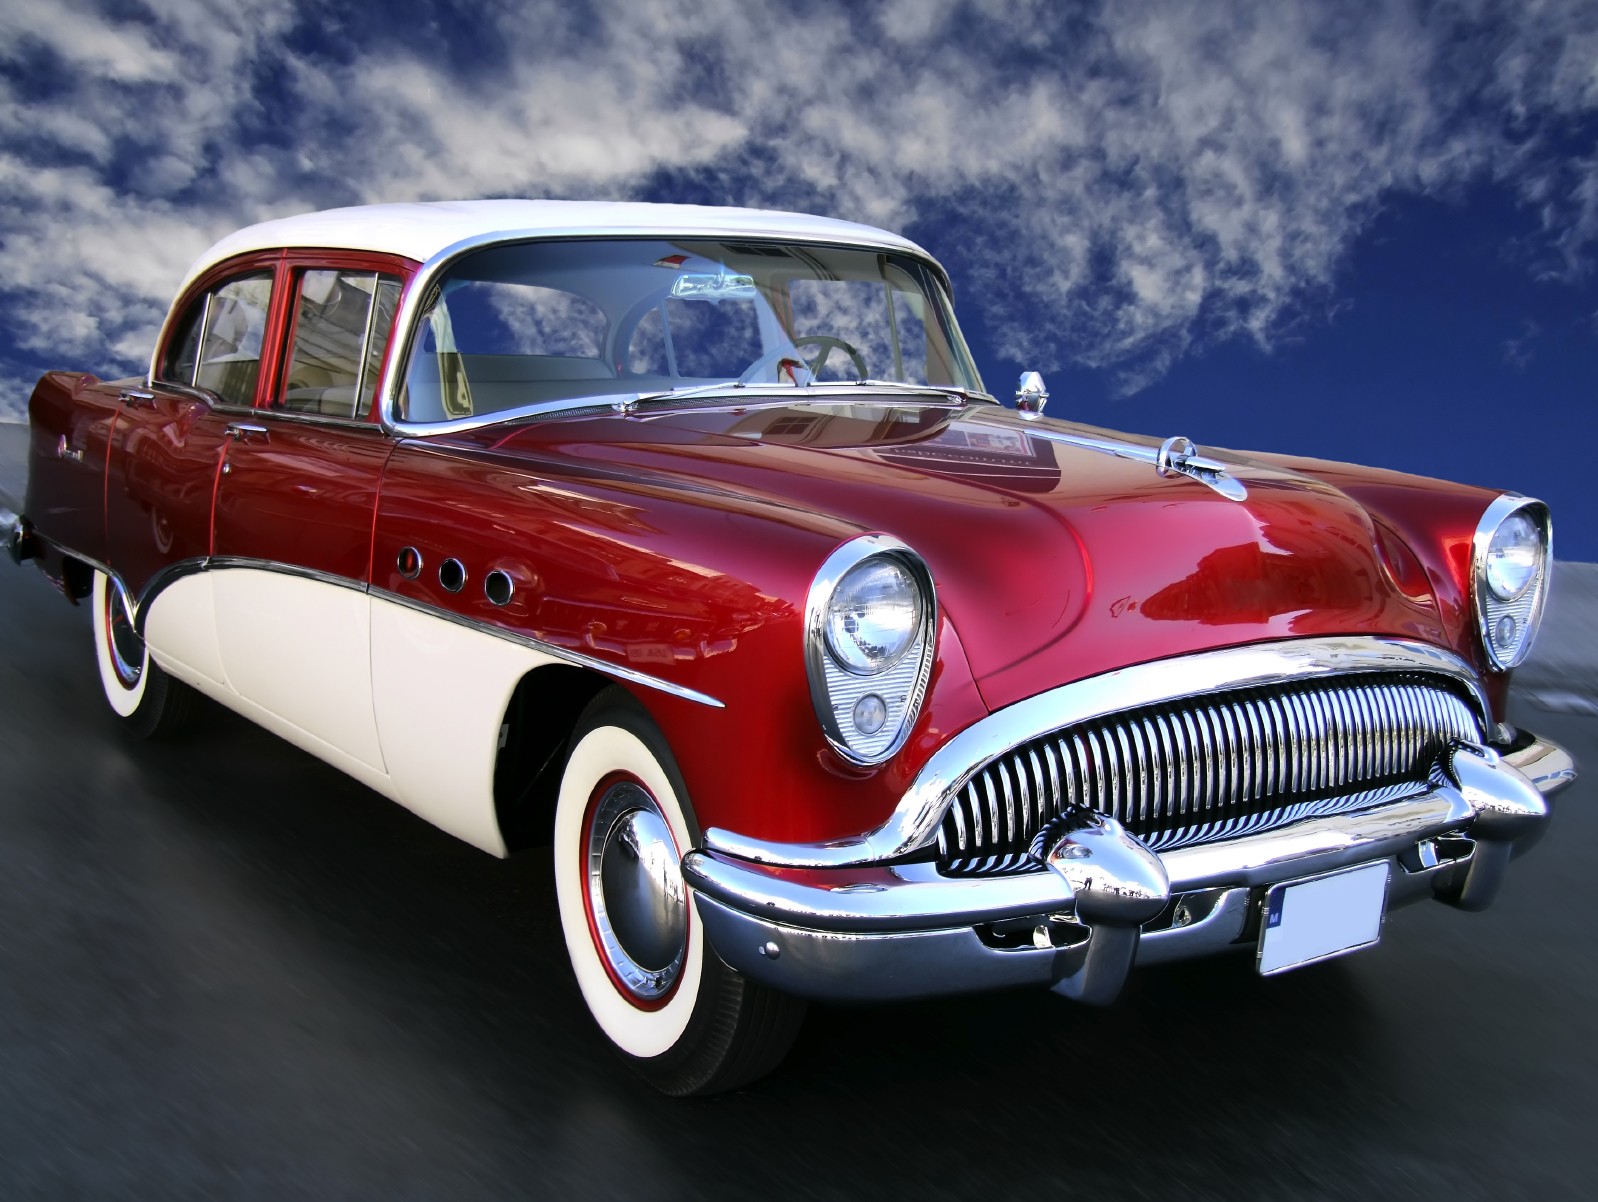
\includegraphics[width=\linewidth]{car.jpg} % orig img num.1
	\end{subfigure}
	\begin{subfigure}[b]{0.3\linewidth}
		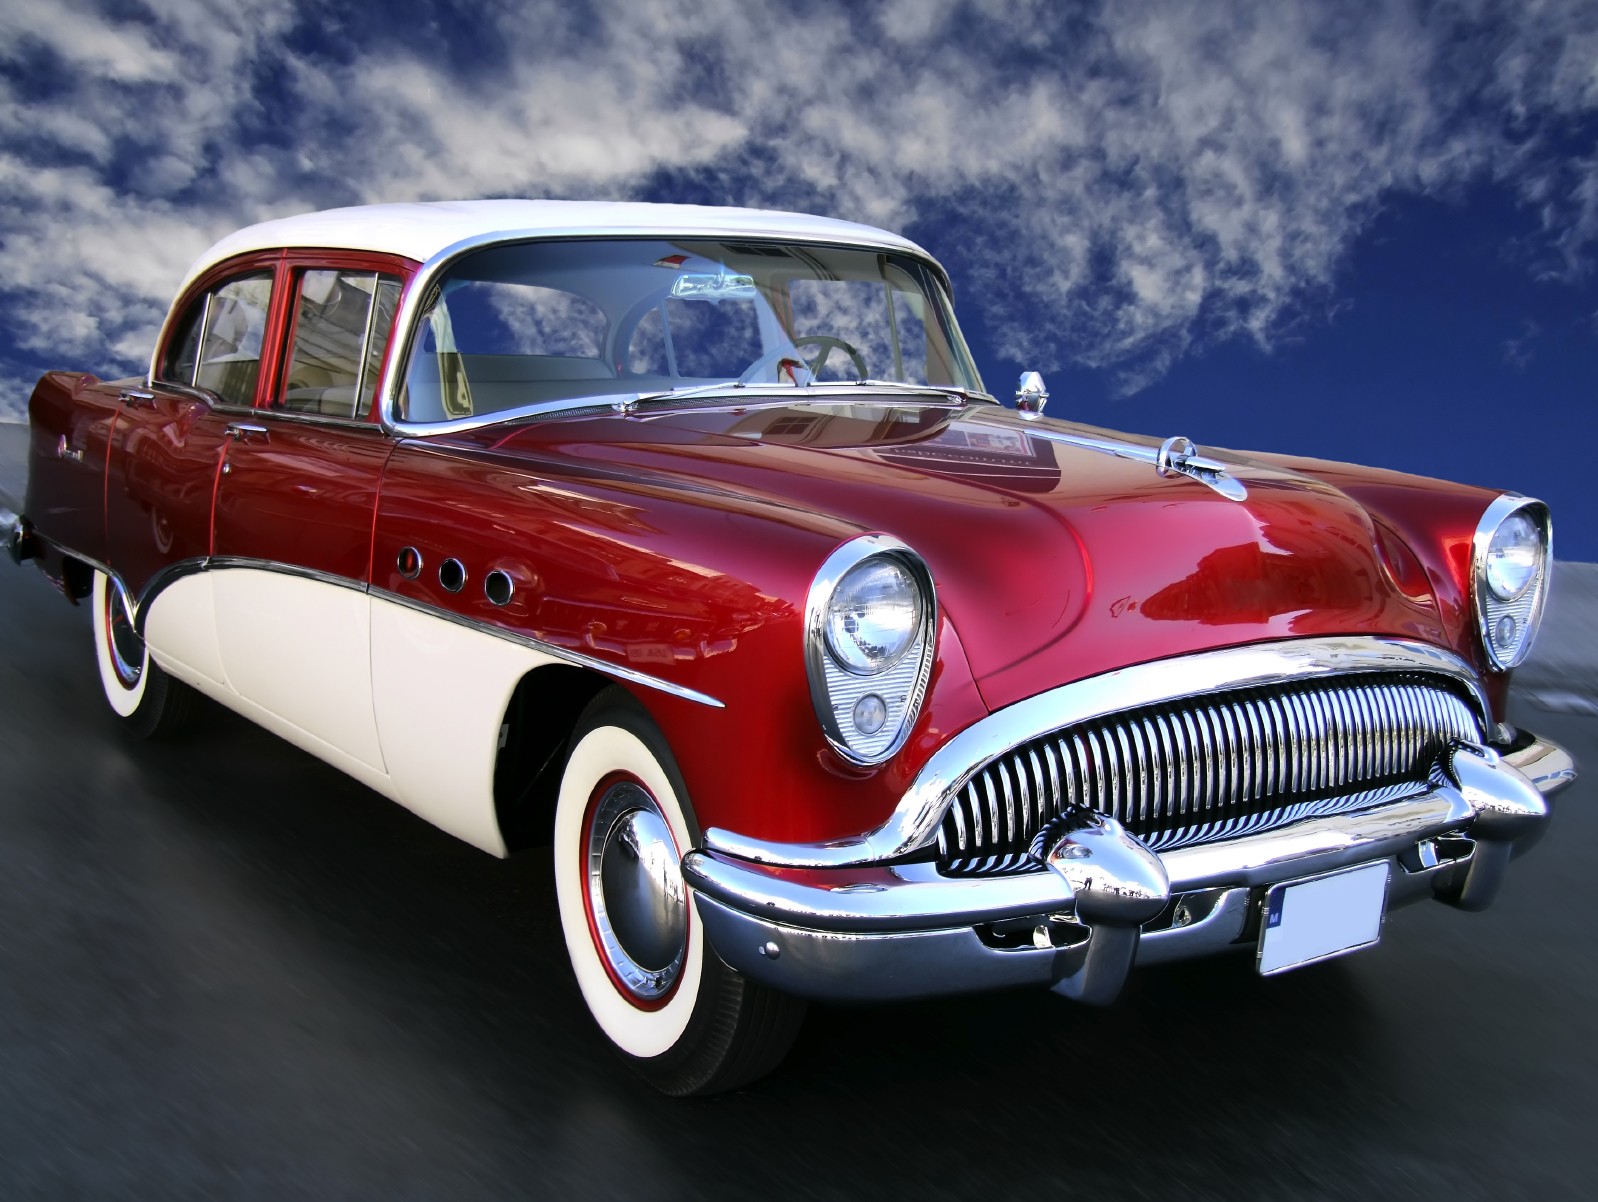
\includegraphics[width=\linewidth]{car.jpg} % our reconstruction num.1	
	\end{subfigure}
	\begin{subfigure}[b]{0.3\linewidth}
		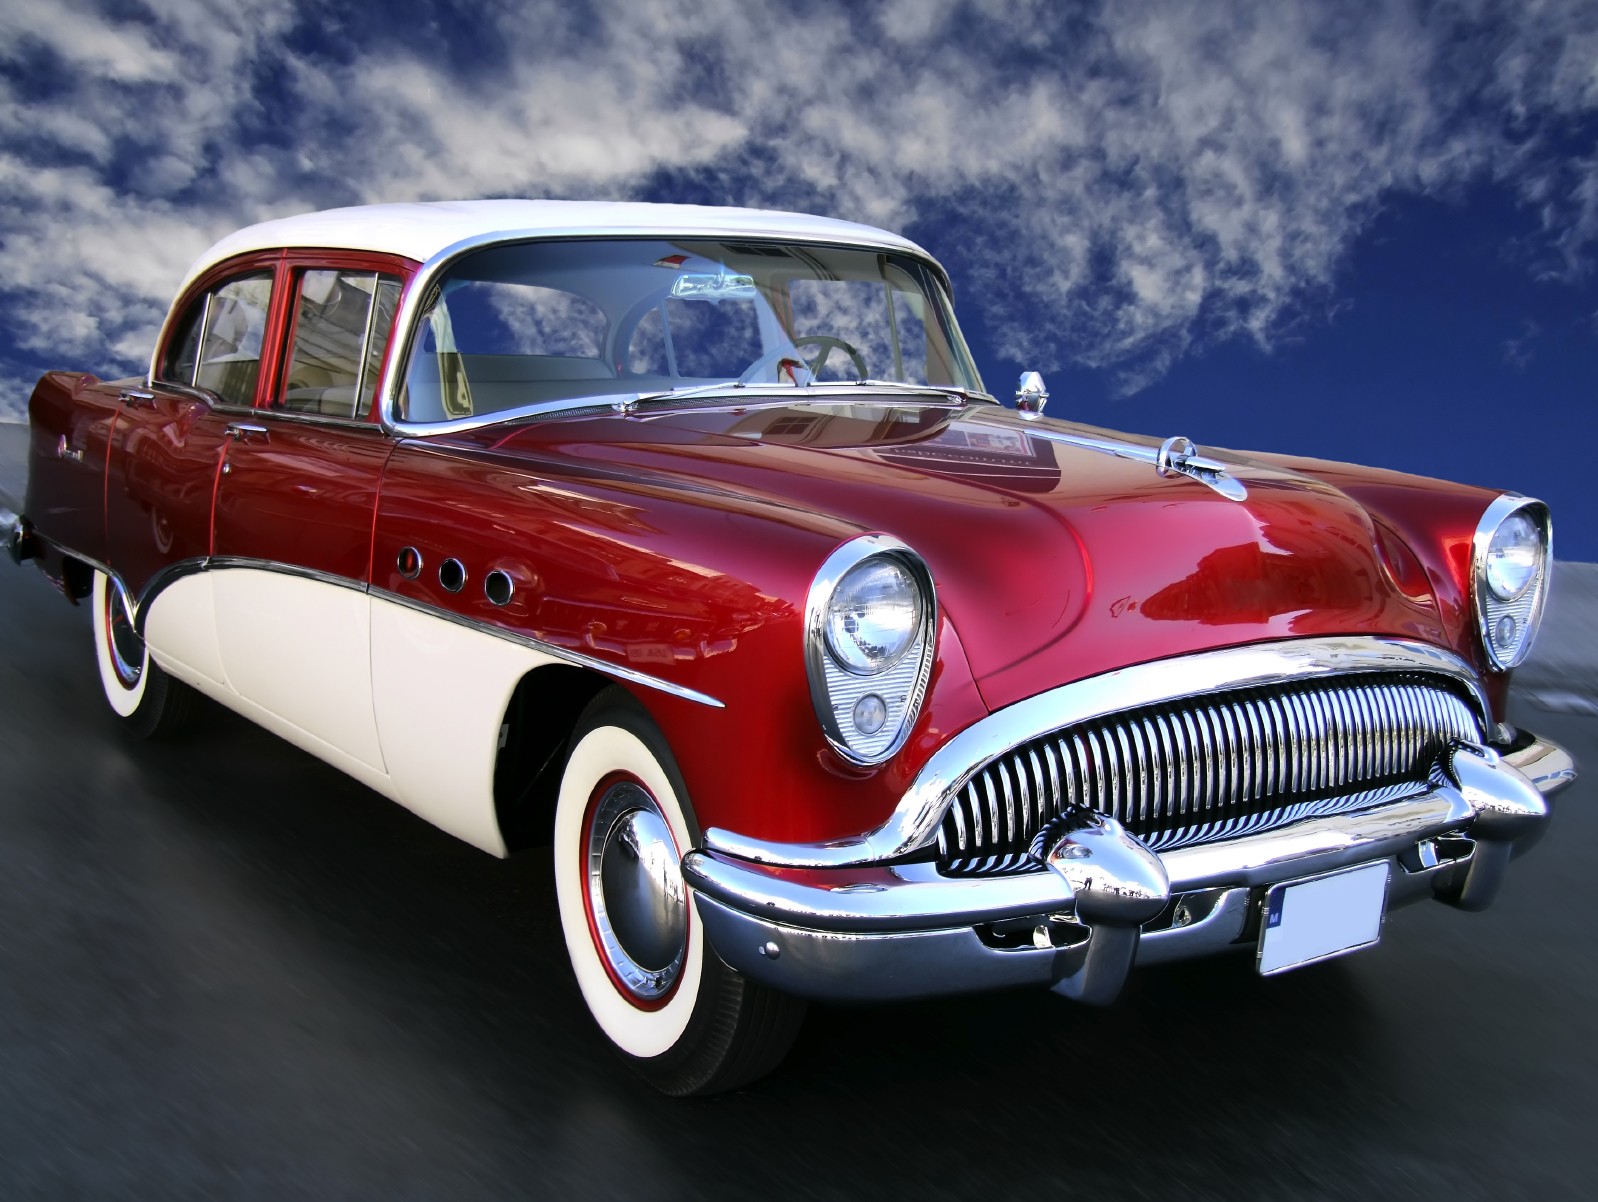
\includegraphics[width=\linewidth]{car.jpg} % their reconstruction num.1	
	\end{subfigure}
% second line
		\centering
	\begin{subfigure}[b]{0.3\linewidth}
		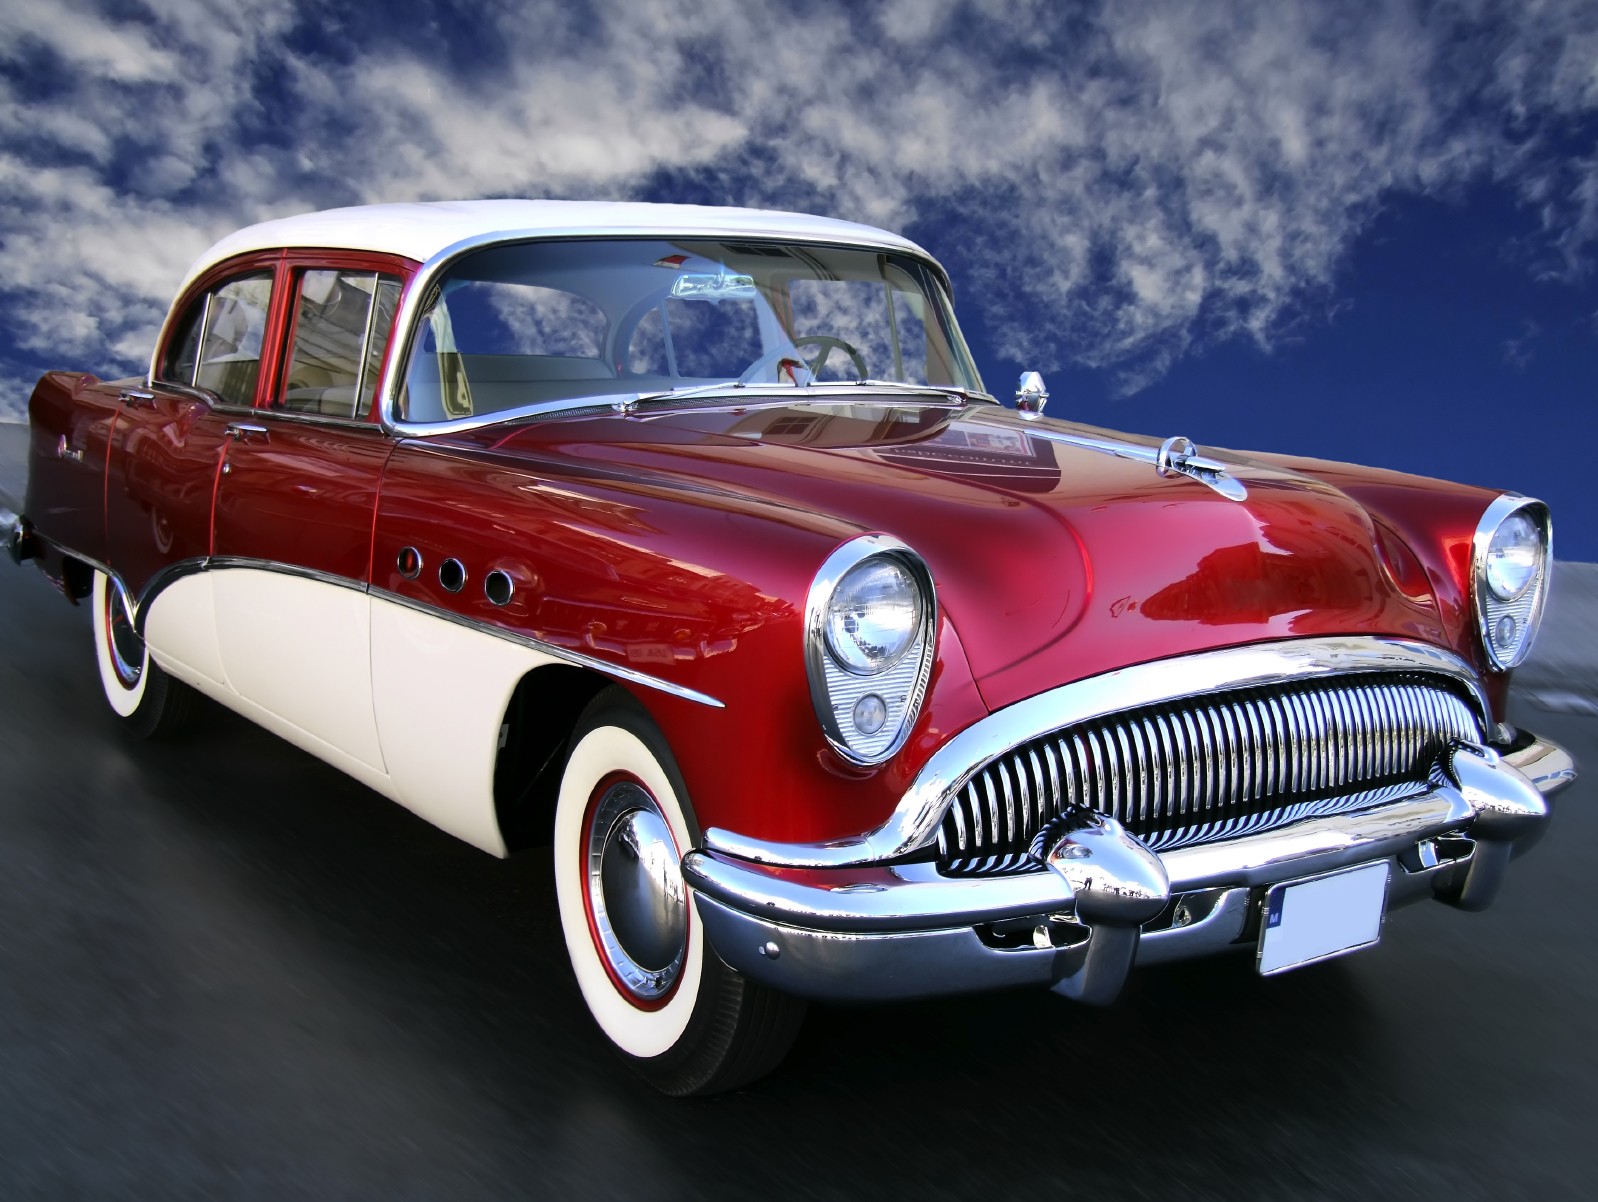
\includegraphics[width=\linewidth]{car.jpg} %orig img num.2
	\end{subfigure}
	\begin{subfigure}[b]{0.3\linewidth}
		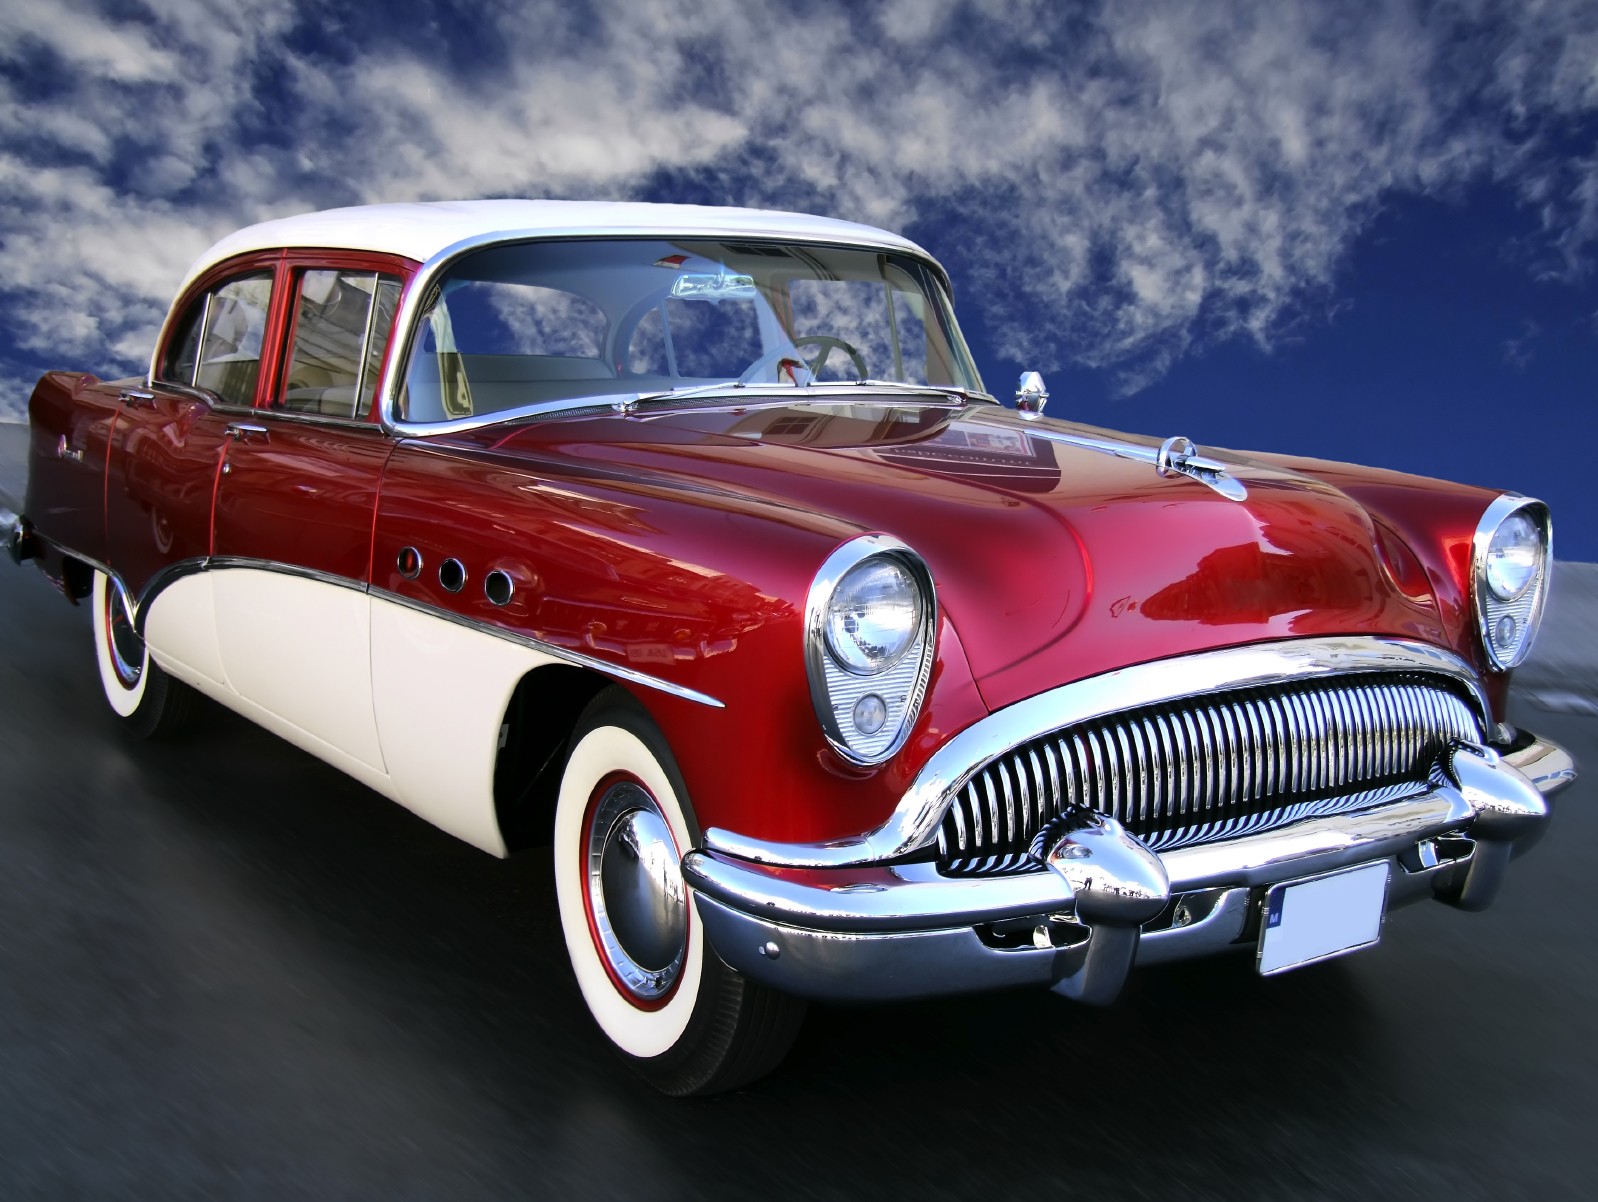
\includegraphics[width=\linewidth]{car.jpg} % our reconstruction num.2
	\end{subfigure}
	\begin{subfigure}[b]{0.3\linewidth}
		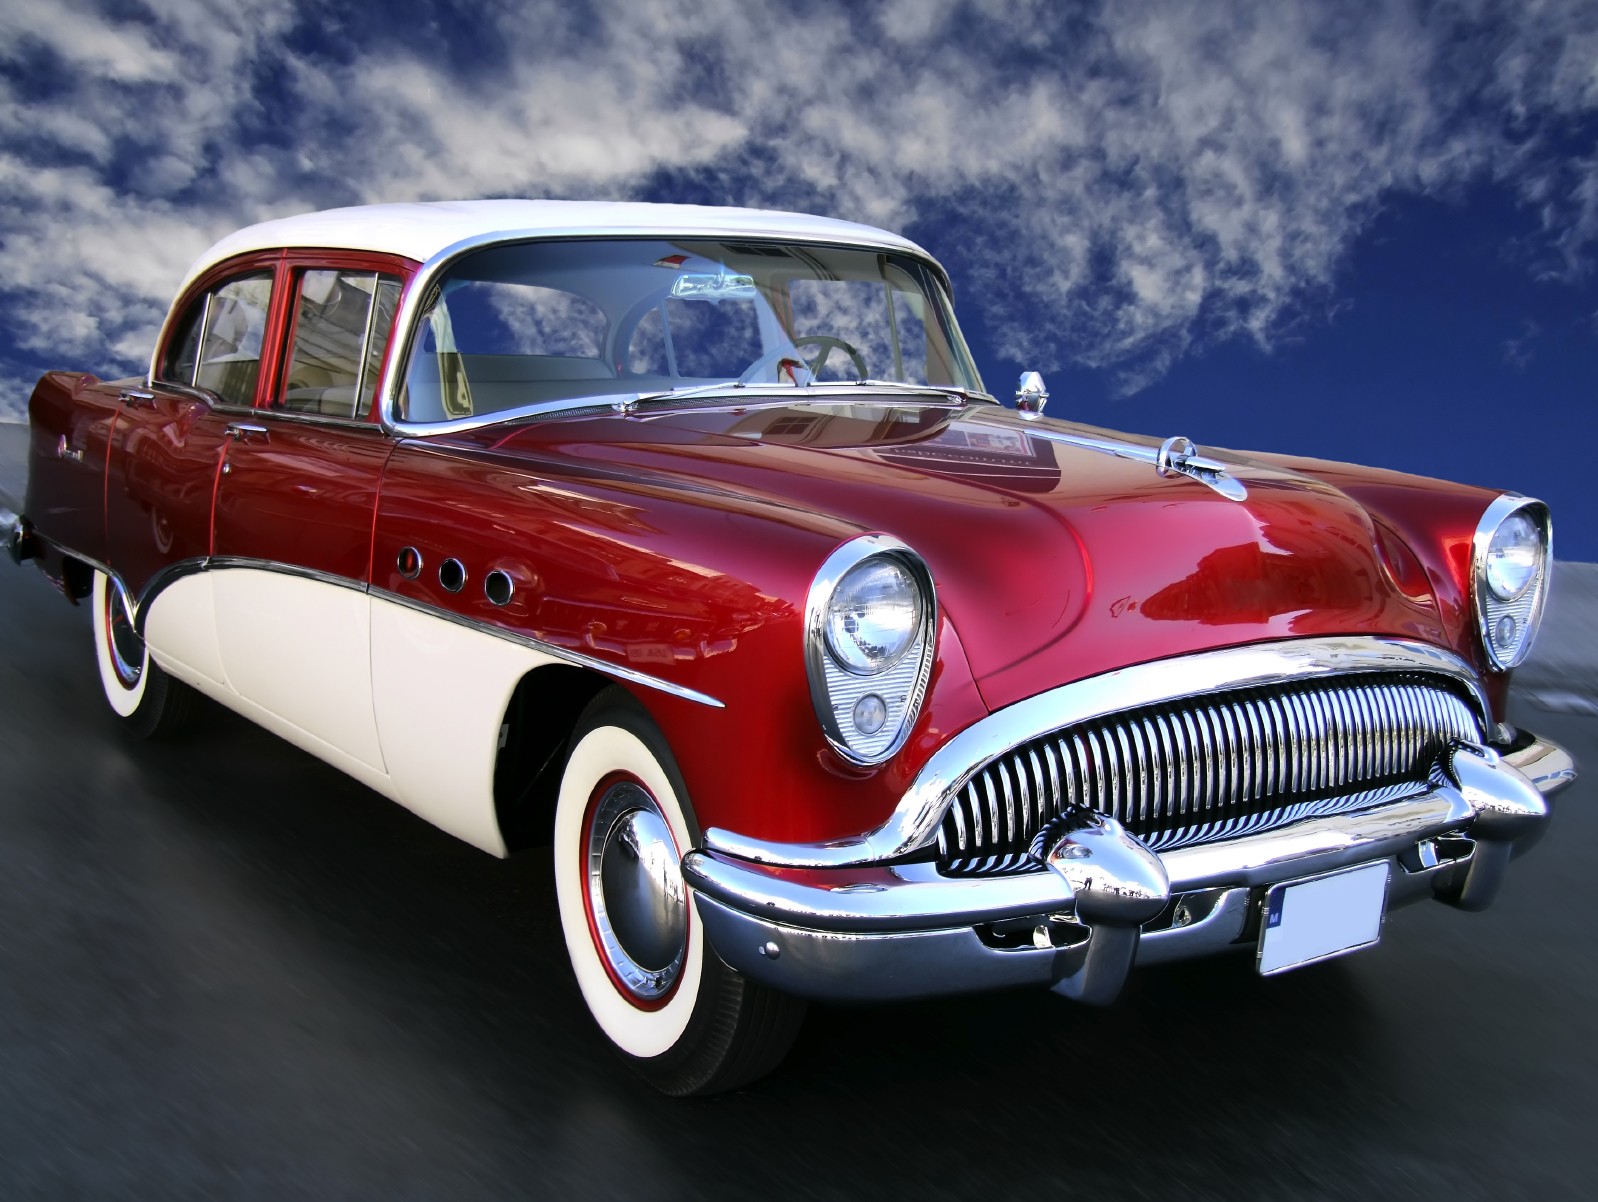
\includegraphics[width=\linewidth]{car.jpg} % their reconstruction num.2
	\end{subfigure}
% third line
		\centering
	\begin{subfigure}[b]{0.3\linewidth}
		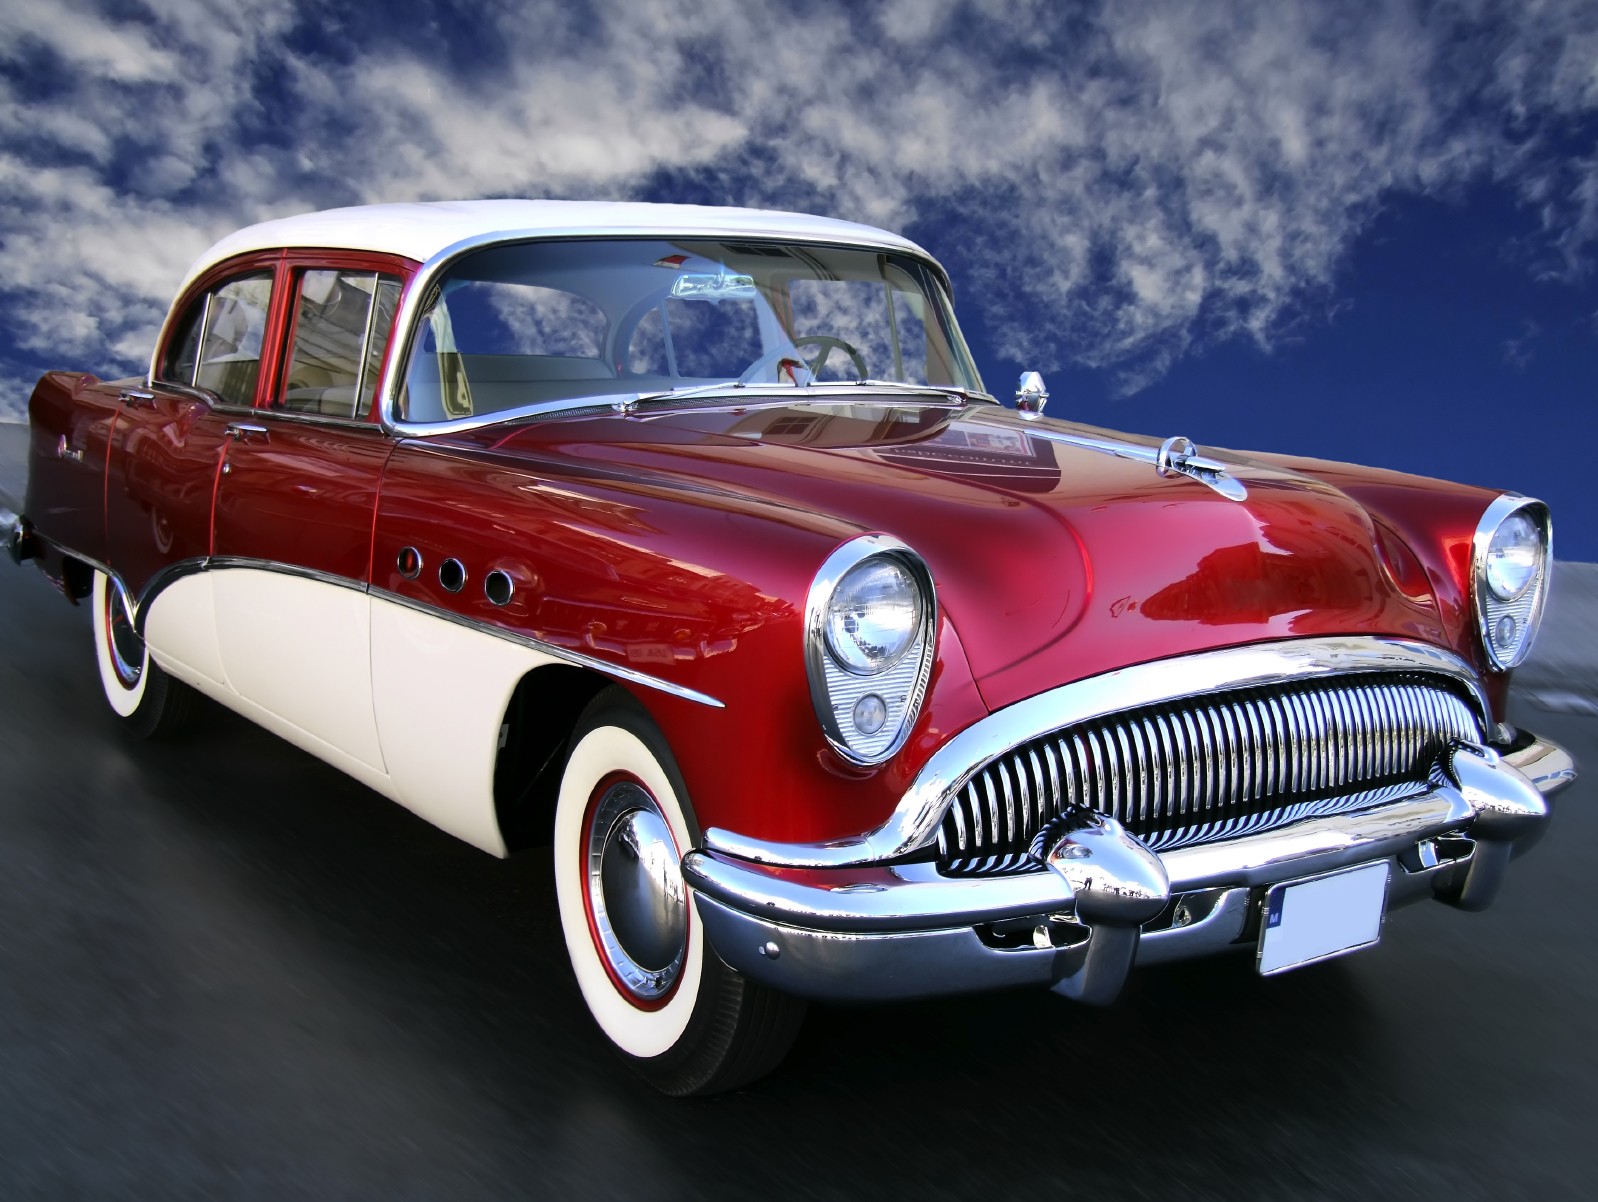
\includegraphics[width=\linewidth]{car.jpg} %orig img num.3
	\end{subfigure}
	\begin{subfigure}[b]{0.3\linewidth}
		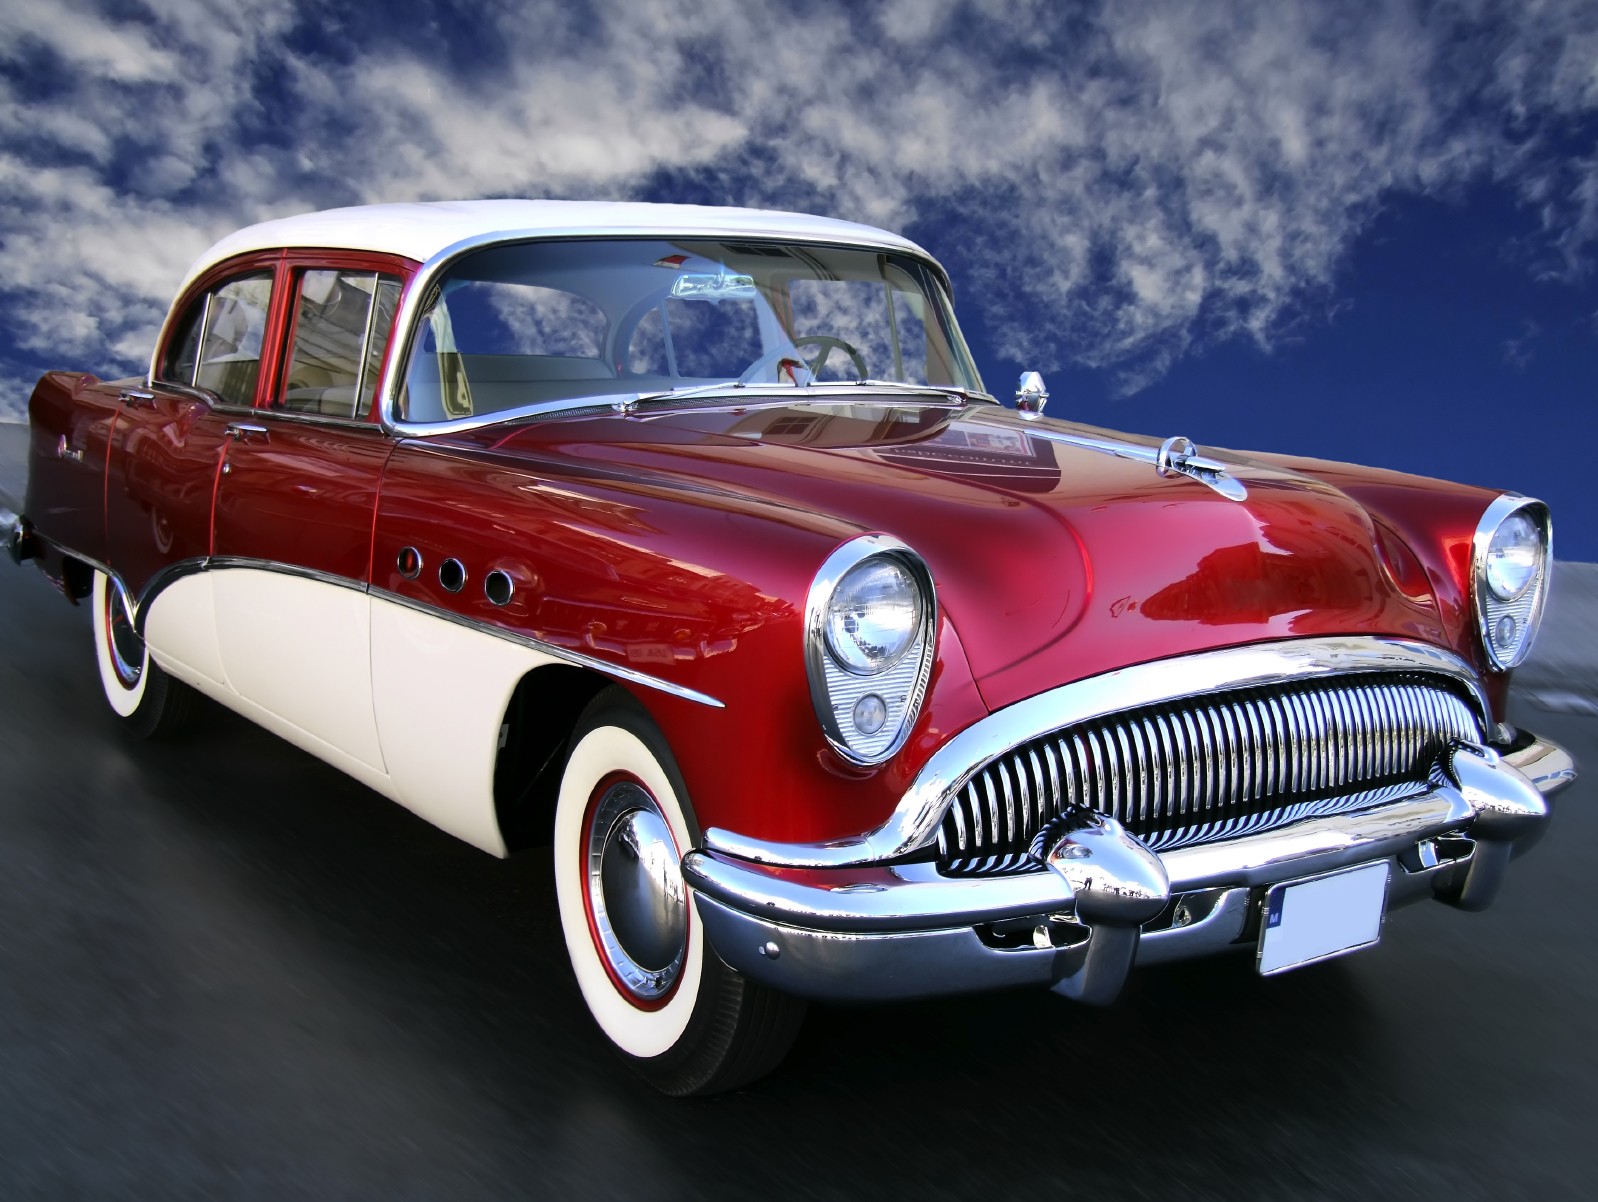
\includegraphics[width=\linewidth]{car.jpg} % our reconstruction num.3
	\end{subfigure}
	\begin{subfigure}[b]{0.3\linewidth}
		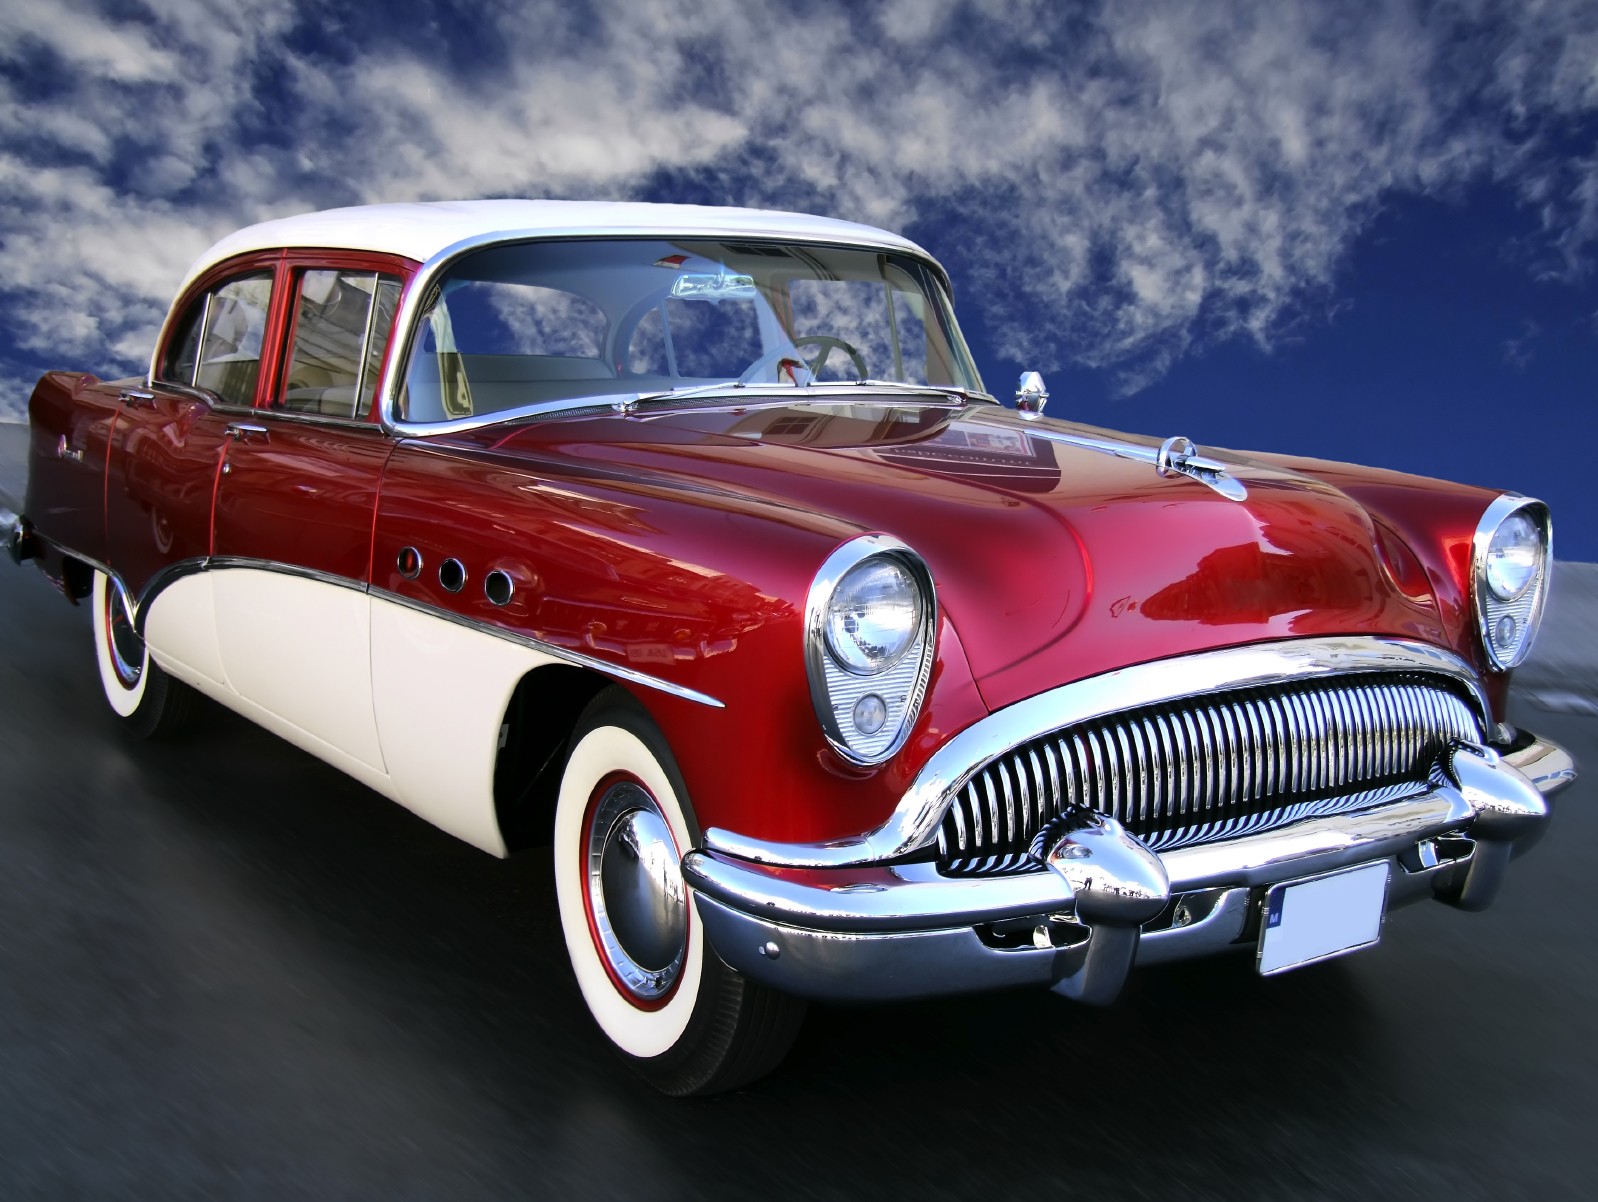
\includegraphics[width=\linewidth]{car.jpg} % their reconstruction num.3
	\end{subfigure}
% fourth line
	\centering
	\begin{subfigure}[b]{0.3\linewidth}
		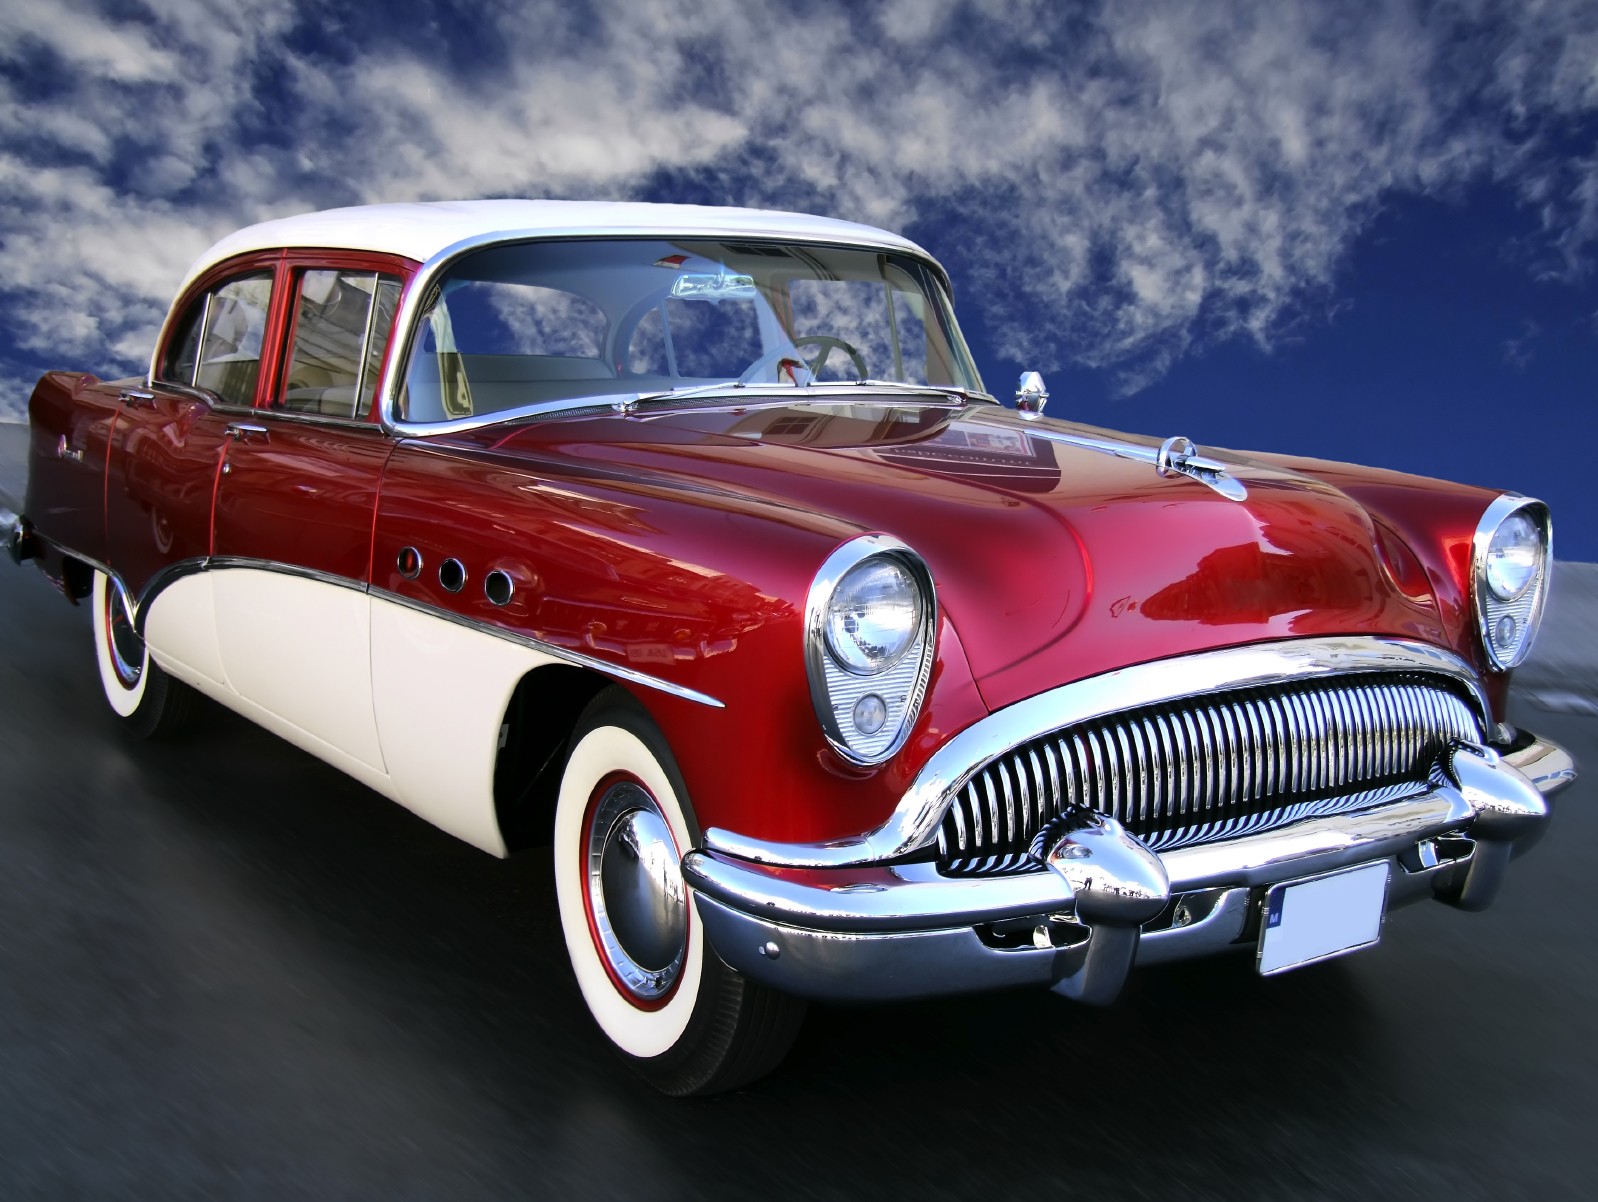
\includegraphics[width=\linewidth]{car.jpg} %orig img num.4
	\end{subfigure}
	\begin{subfigure}[b]{0.3\linewidth}
		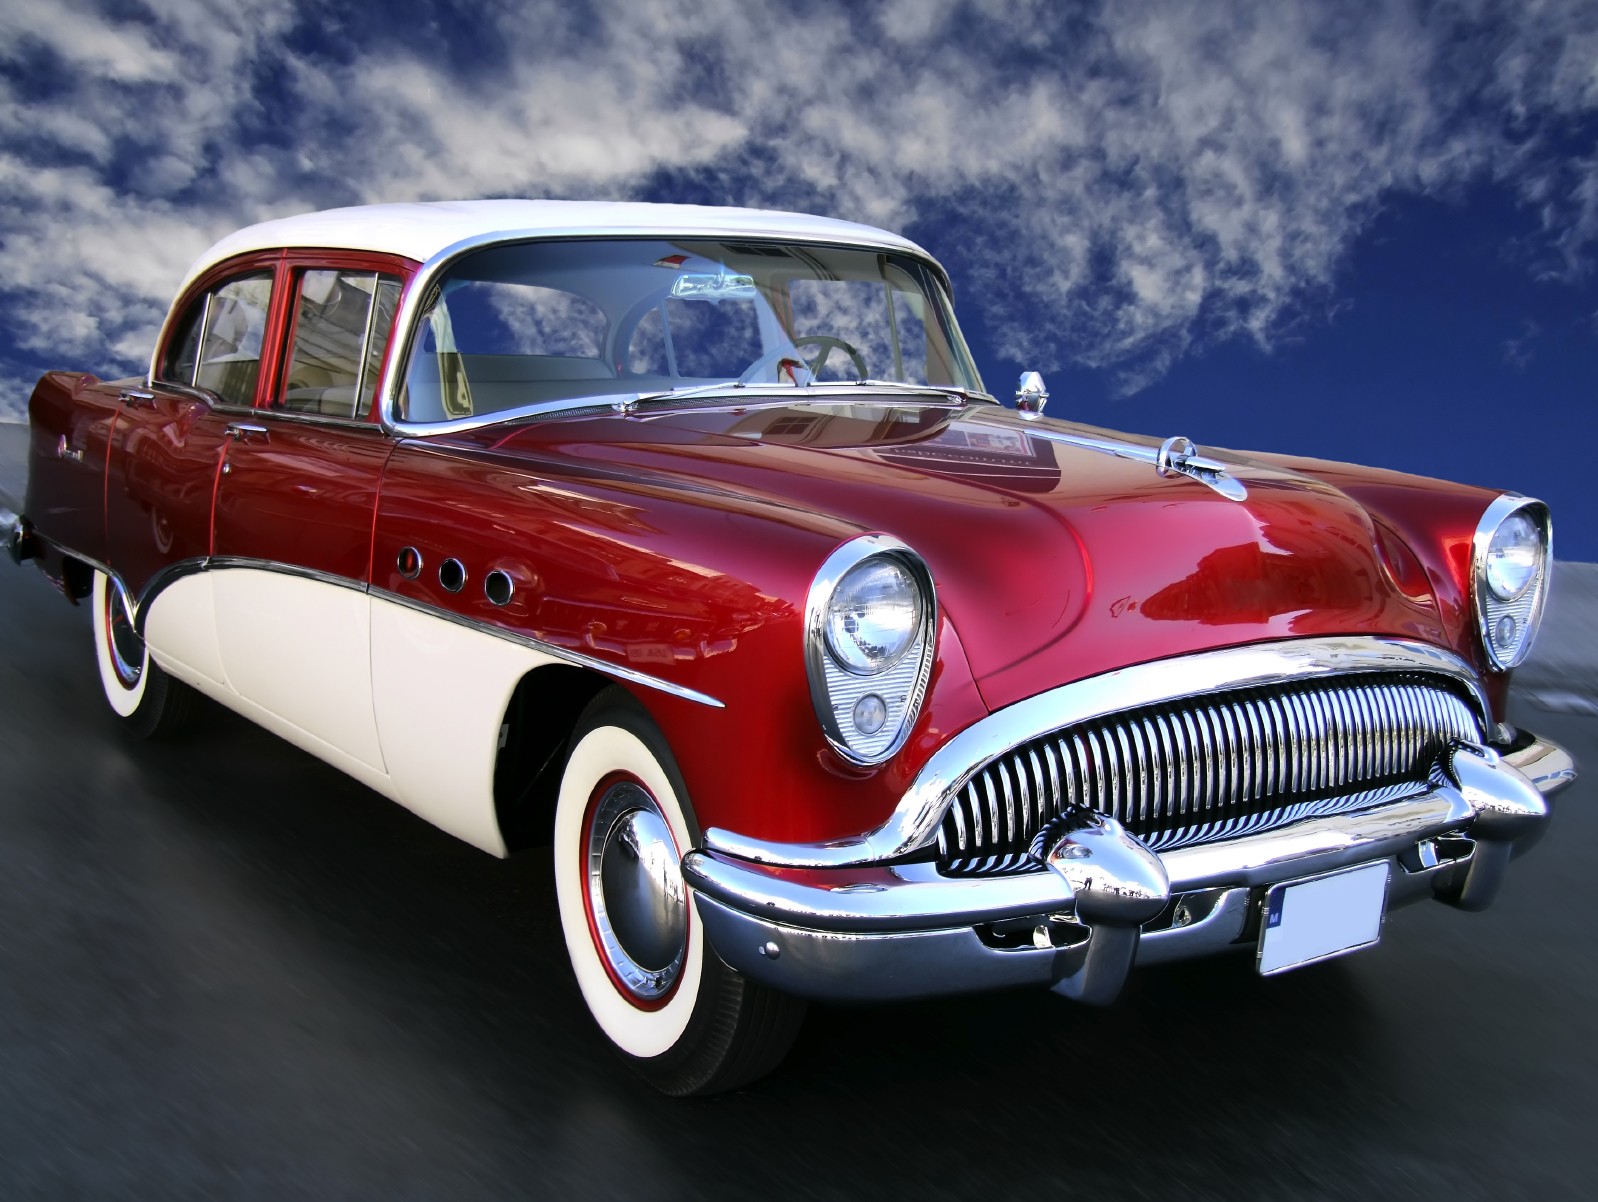
\includegraphics[width=\linewidth]{car.jpg} % our reconstruction num.4
	\end{subfigure}
	\begin{subfigure}[b]{0.3\linewidth}
		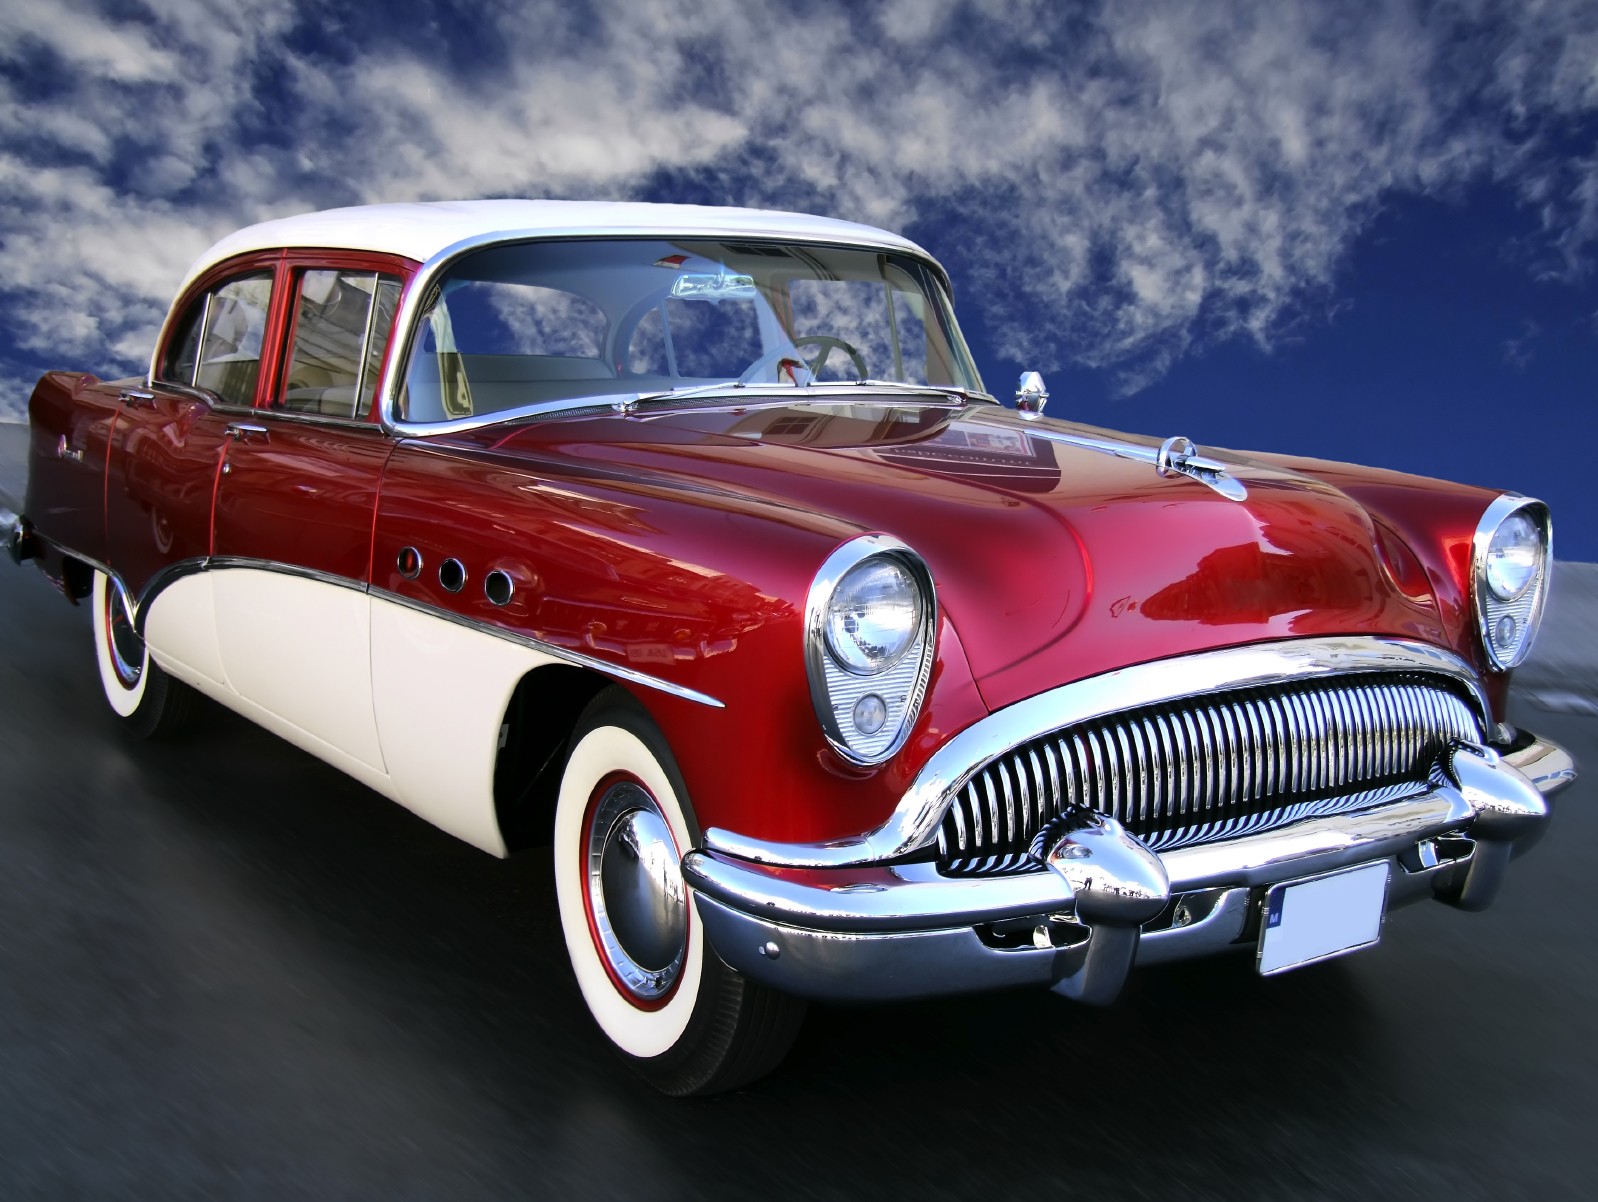
\includegraphics[width=\linewidth]{car.jpg} % their reconstruction num.4
	\end{subfigure}
% fifth line
		\centering
	\begin{subfigure}[b]{0.3\linewidth}
		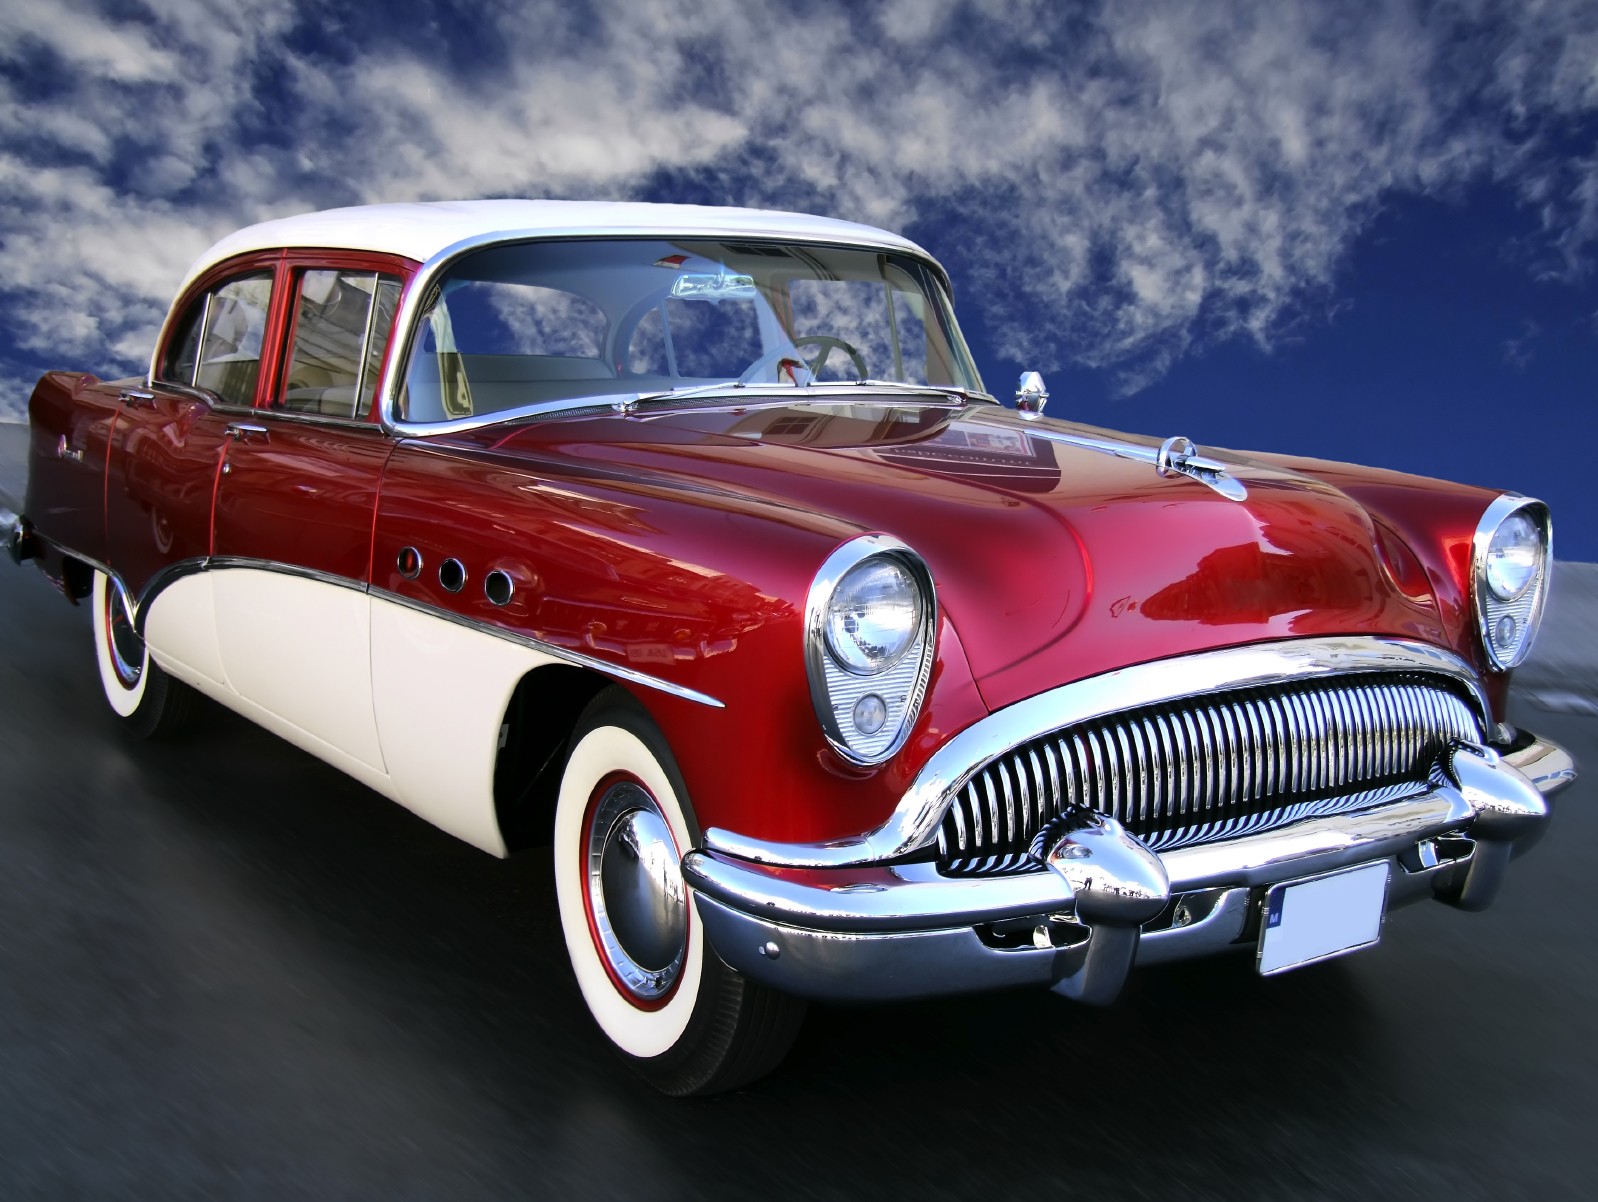
\includegraphics[width=\linewidth]{car.jpg} %orig img num.5
		\caption{Original}
	\end{subfigure}
	\begin{subfigure}[b]{0.3\linewidth}
		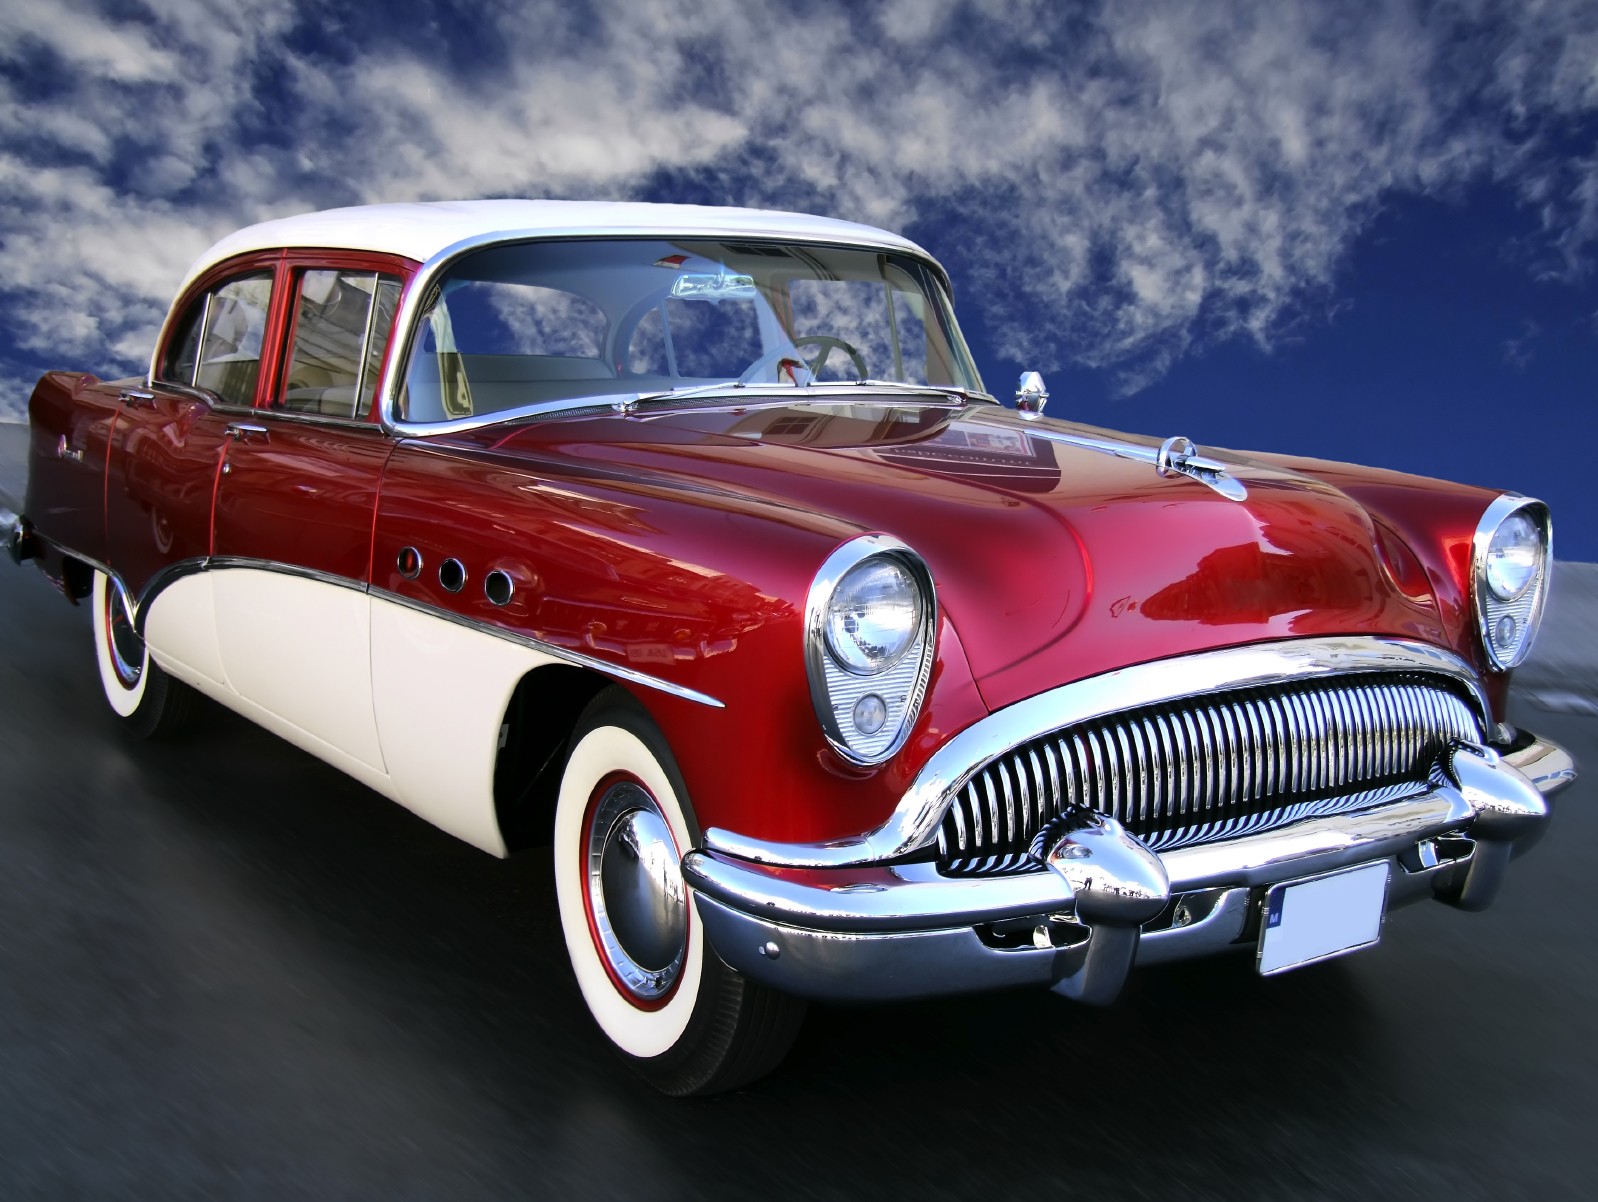
\includegraphics[width=\linewidth]{car.jpg} % our reconstruction num.5
		\caption{Our reconstruction}
	\end{subfigure}
	\begin{subfigure}[b]{0.3\linewidth}
		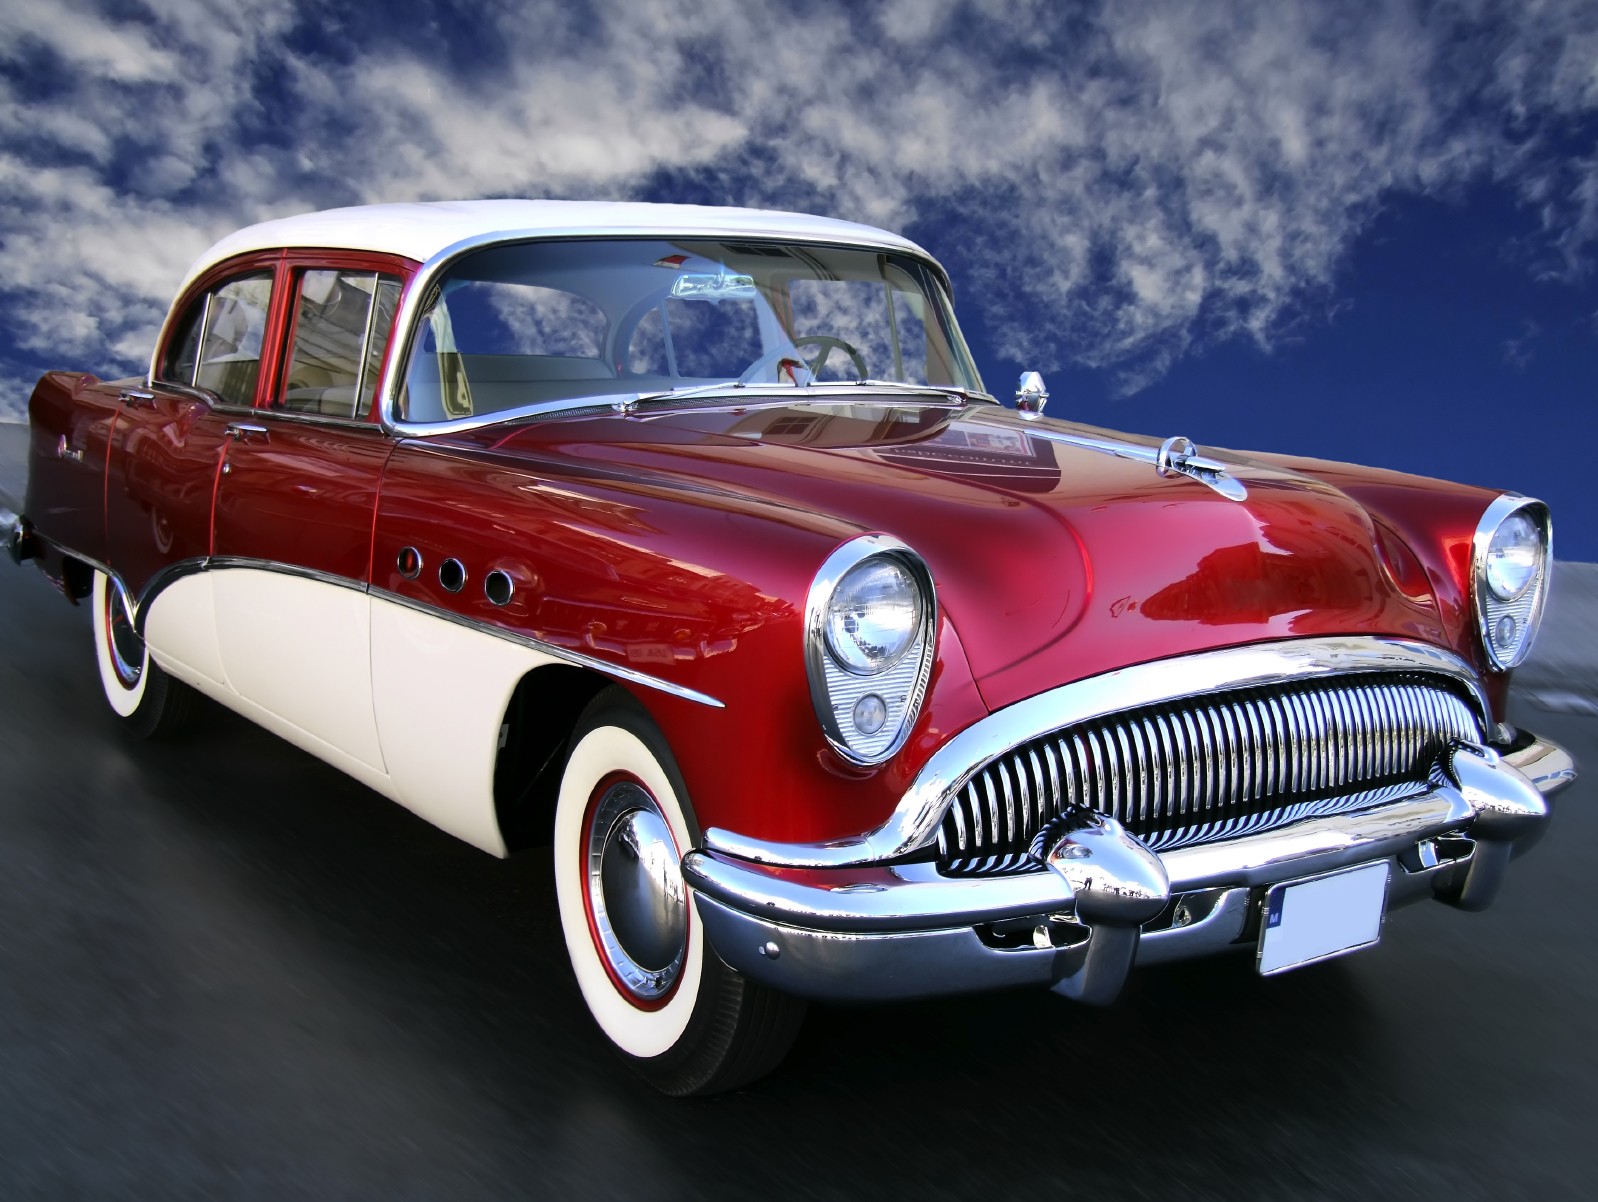
\includegraphics[width=\linewidth]{car.jpg} % their reconstruction num.5
		\caption{Li et al. \cite{bib11} decoder}	
	\end{subfigure}
	\caption{Reconstructed images using different trained decoders}
	\label{fig:reconstruction}
\end{figure}
To demonstrate the performance of our trained decoder on the Microsoft COCO dataset \cite{bib10}, we take 5 different images as an input to our decoder as well as to UST's article decoder in order to visualize the quality of the reconstructed images as presented in figure ~\ref{fig:reconstruction}).\newline
%%%%%%%%
%we can tell here that we didn't have much time and compute power to handle such a training, hene our decoders...
%%%%%%%%

% ecoder-decoder table %
\begin{flushleft}
\textbf{4.2 Encoder-Decoder reconstruction}\newline
\begin{flushleft}
\centering
Table 1: Reconstruction distortion Loss comparison for each architecture
\begin{tabular}{ |p{2cm}||p{2cm}|p{2cm}|p{2cm}|p{2cm}| }
	\hline
	\multicolumn{5}{|c|}{needs to split this col to two cols for pixel loss and feature loss } \\
	\hline
	architecture &Li et al. \cite{bib11} &Proposed &Li et al. \cite{bib11} &Proposed \\
	\hline
	\centering 1  &	     &  &004 &number\\
	\hline
	\centering 2 &AX  &ALA   &248 &number\\
	\hline
	\centering 3 &AX  &ALA   &248 &number\\
	\hline
	\centering 4 &AX  &ALA   &248 &number\\
	\hline
	\centering 5 &AX  &ALA   &248 &number\\
	\hline
\end{tabular}\\
% style transfer images %
\begin{flushleft}
\textbf{4.3 style transfer}\newline
\end{flushleft}
\begin{figure}[h!]
	% first line
	\centering
	\begin{subfigure}[b]{0.225\linewidth}
		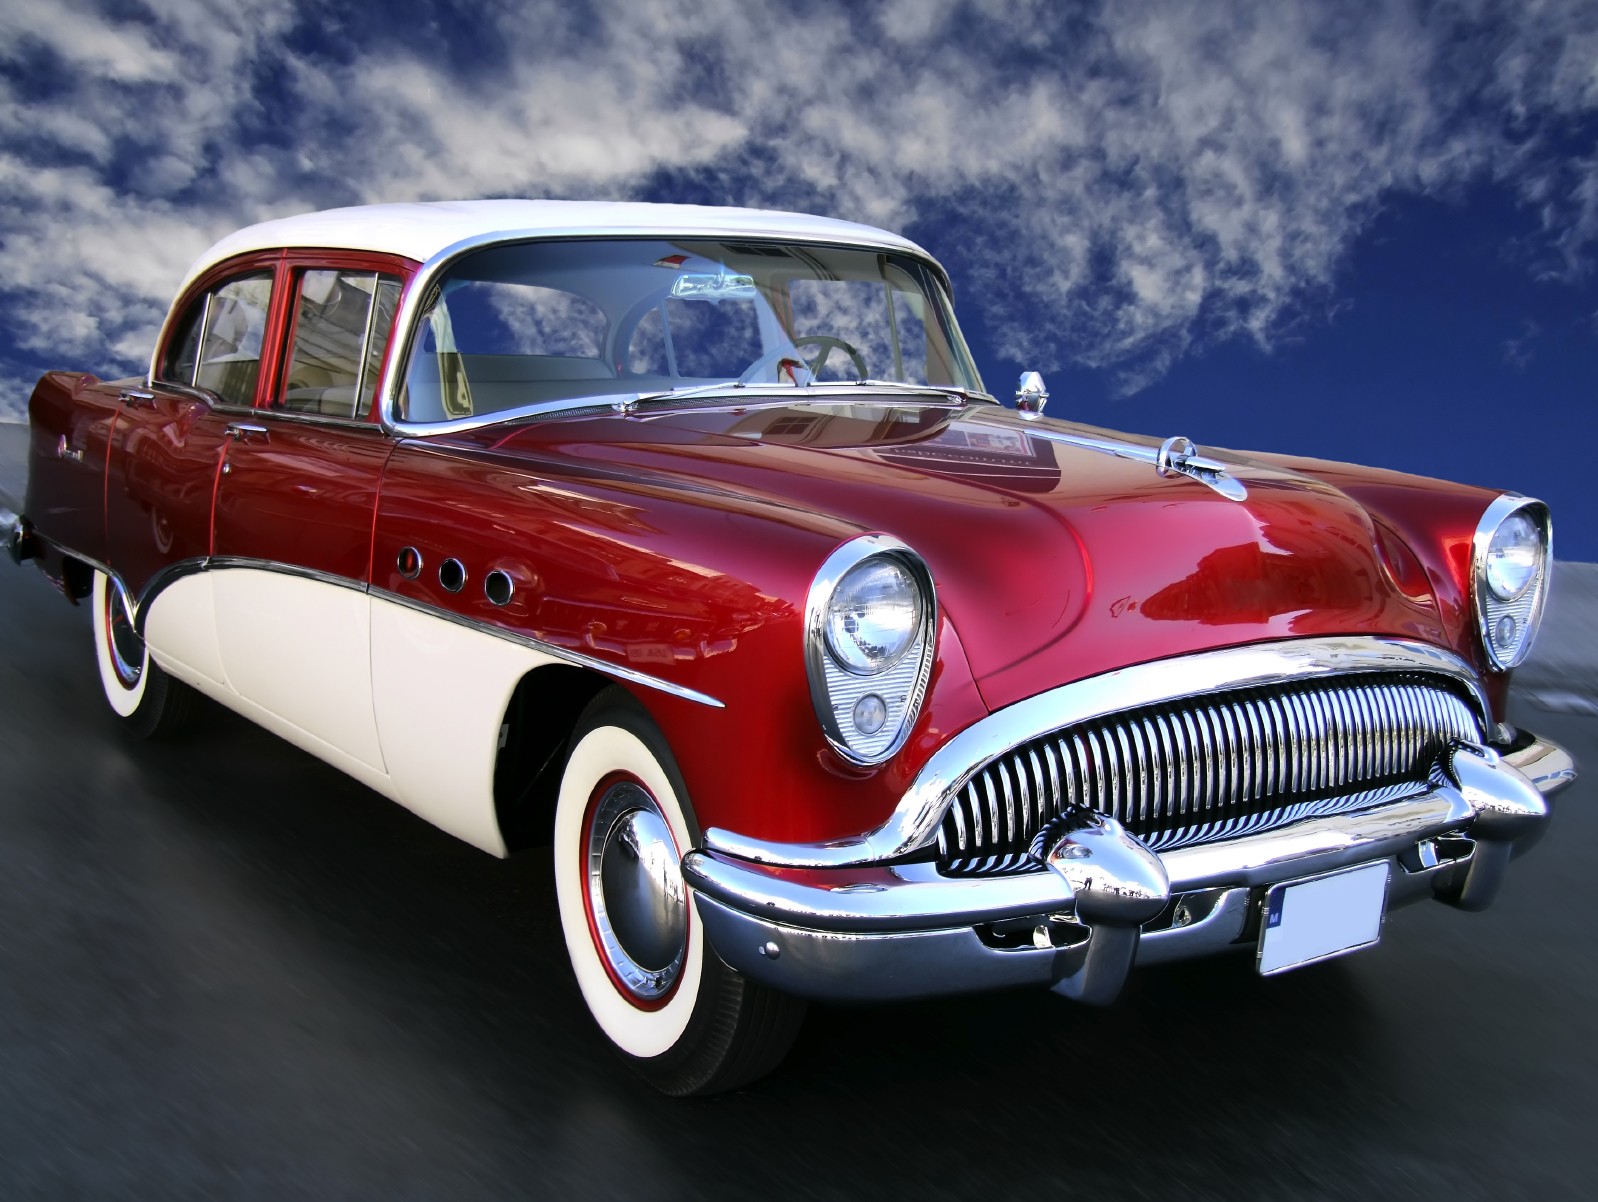
\includegraphics[width=\linewidth]{car.jpg} % style img num.1
	\end{subfigure}
	\begin{subfigure}[b]{0.225\linewidth}
		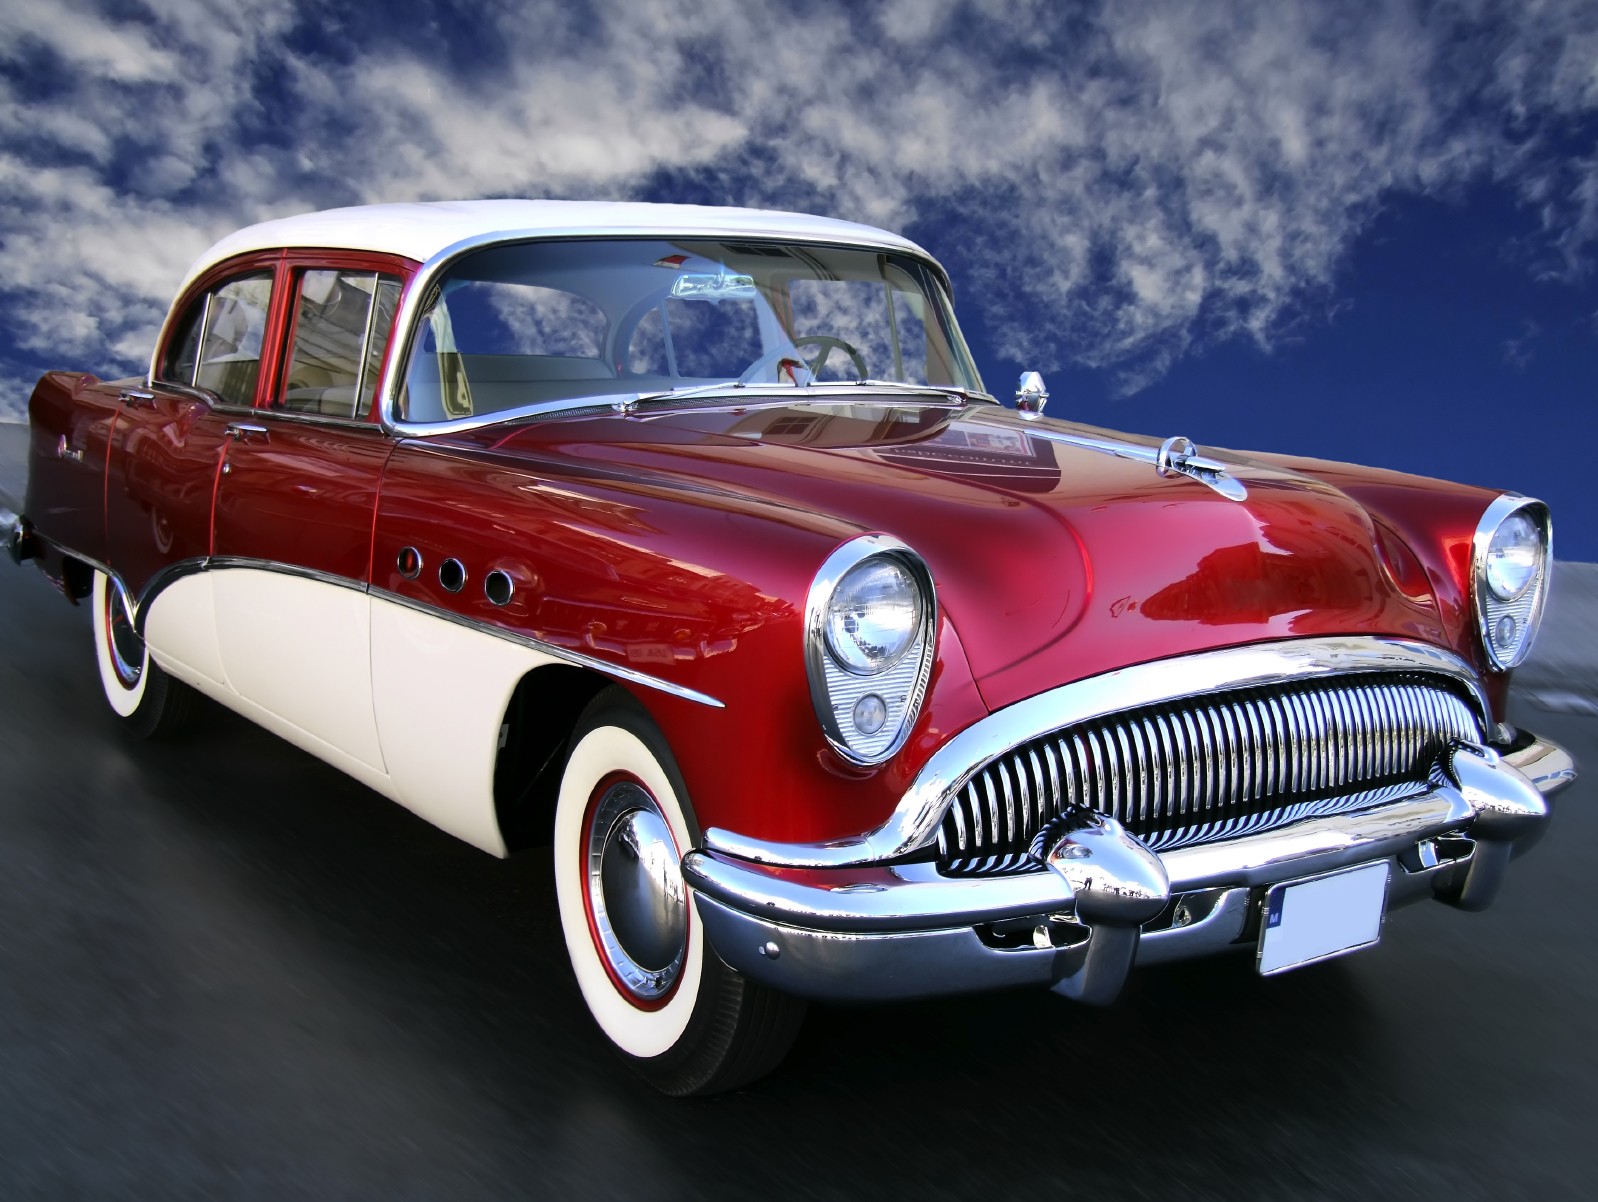
\includegraphics[width=\linewidth]{car.jpg} % content img num.1	
	\end{subfigure}
	\begin{subfigure}[b]{0.225\linewidth}
		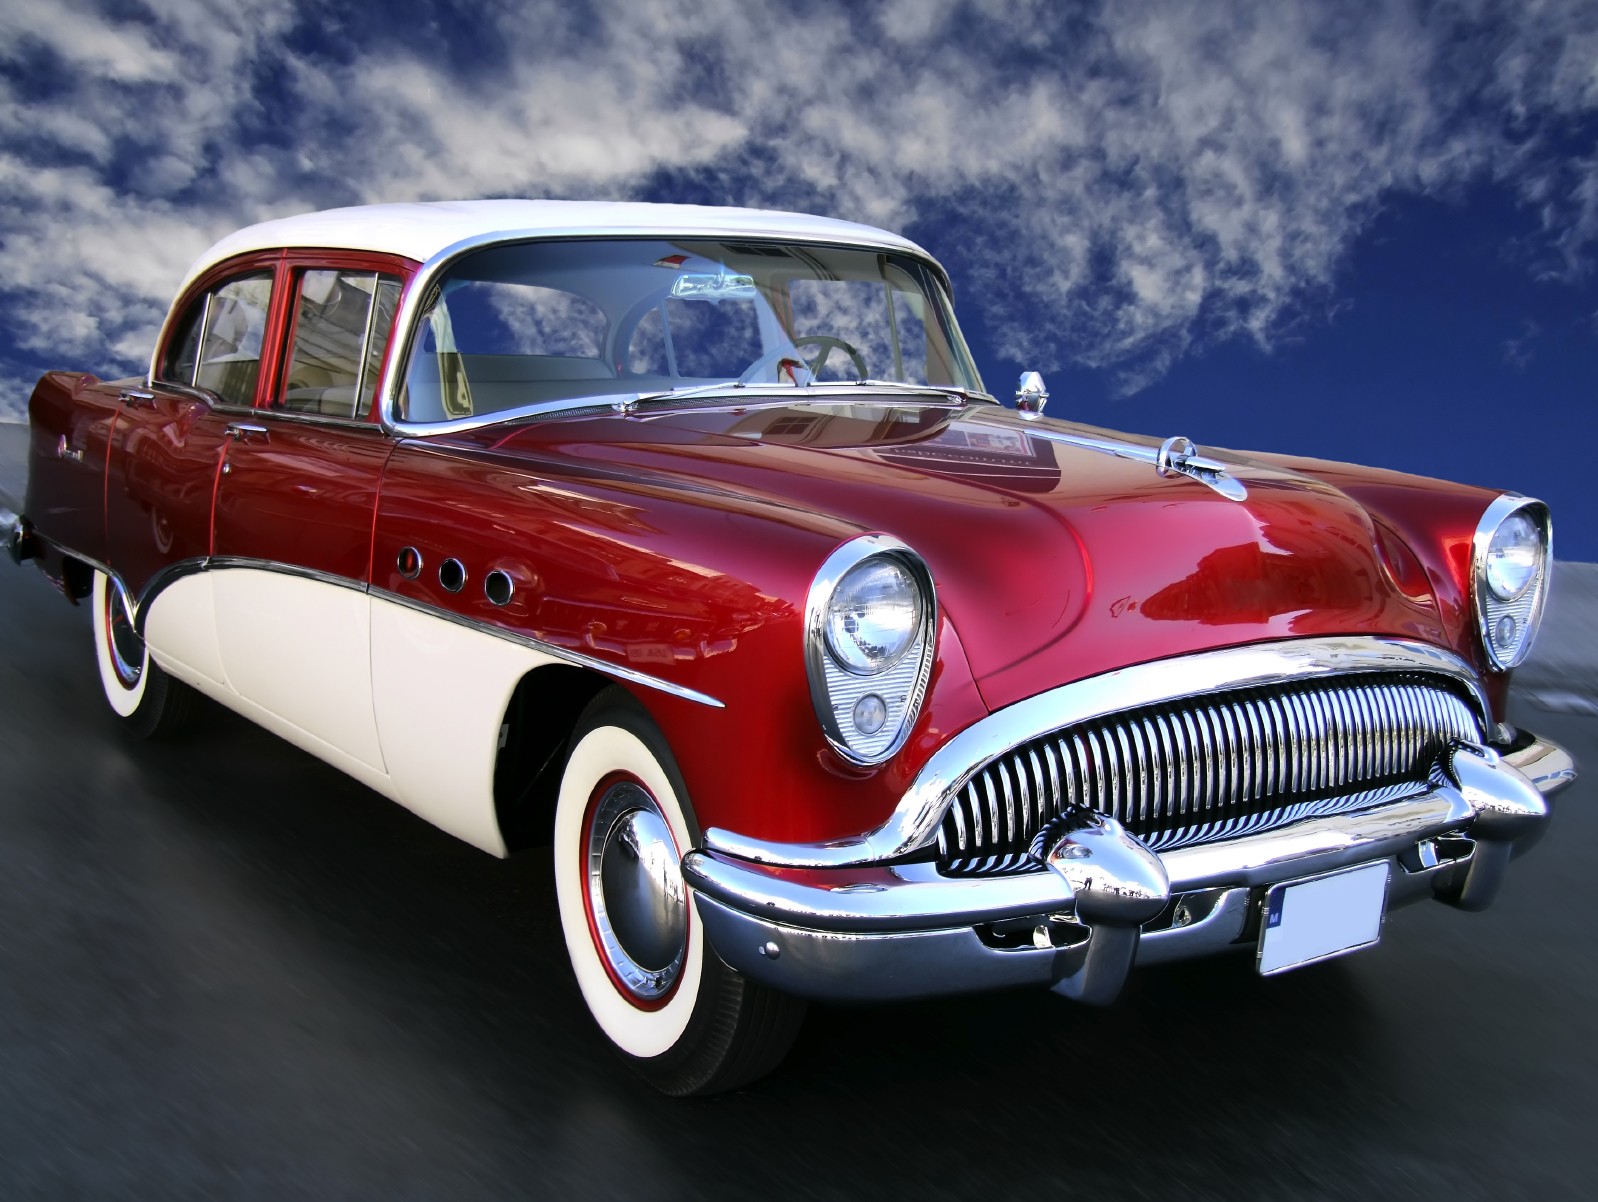
\includegraphics[width=\linewidth]{car.jpg} % theirs reconstruction num.1	
	\end{subfigure}
	\begin{subfigure}[b]{0.225\linewidth}
		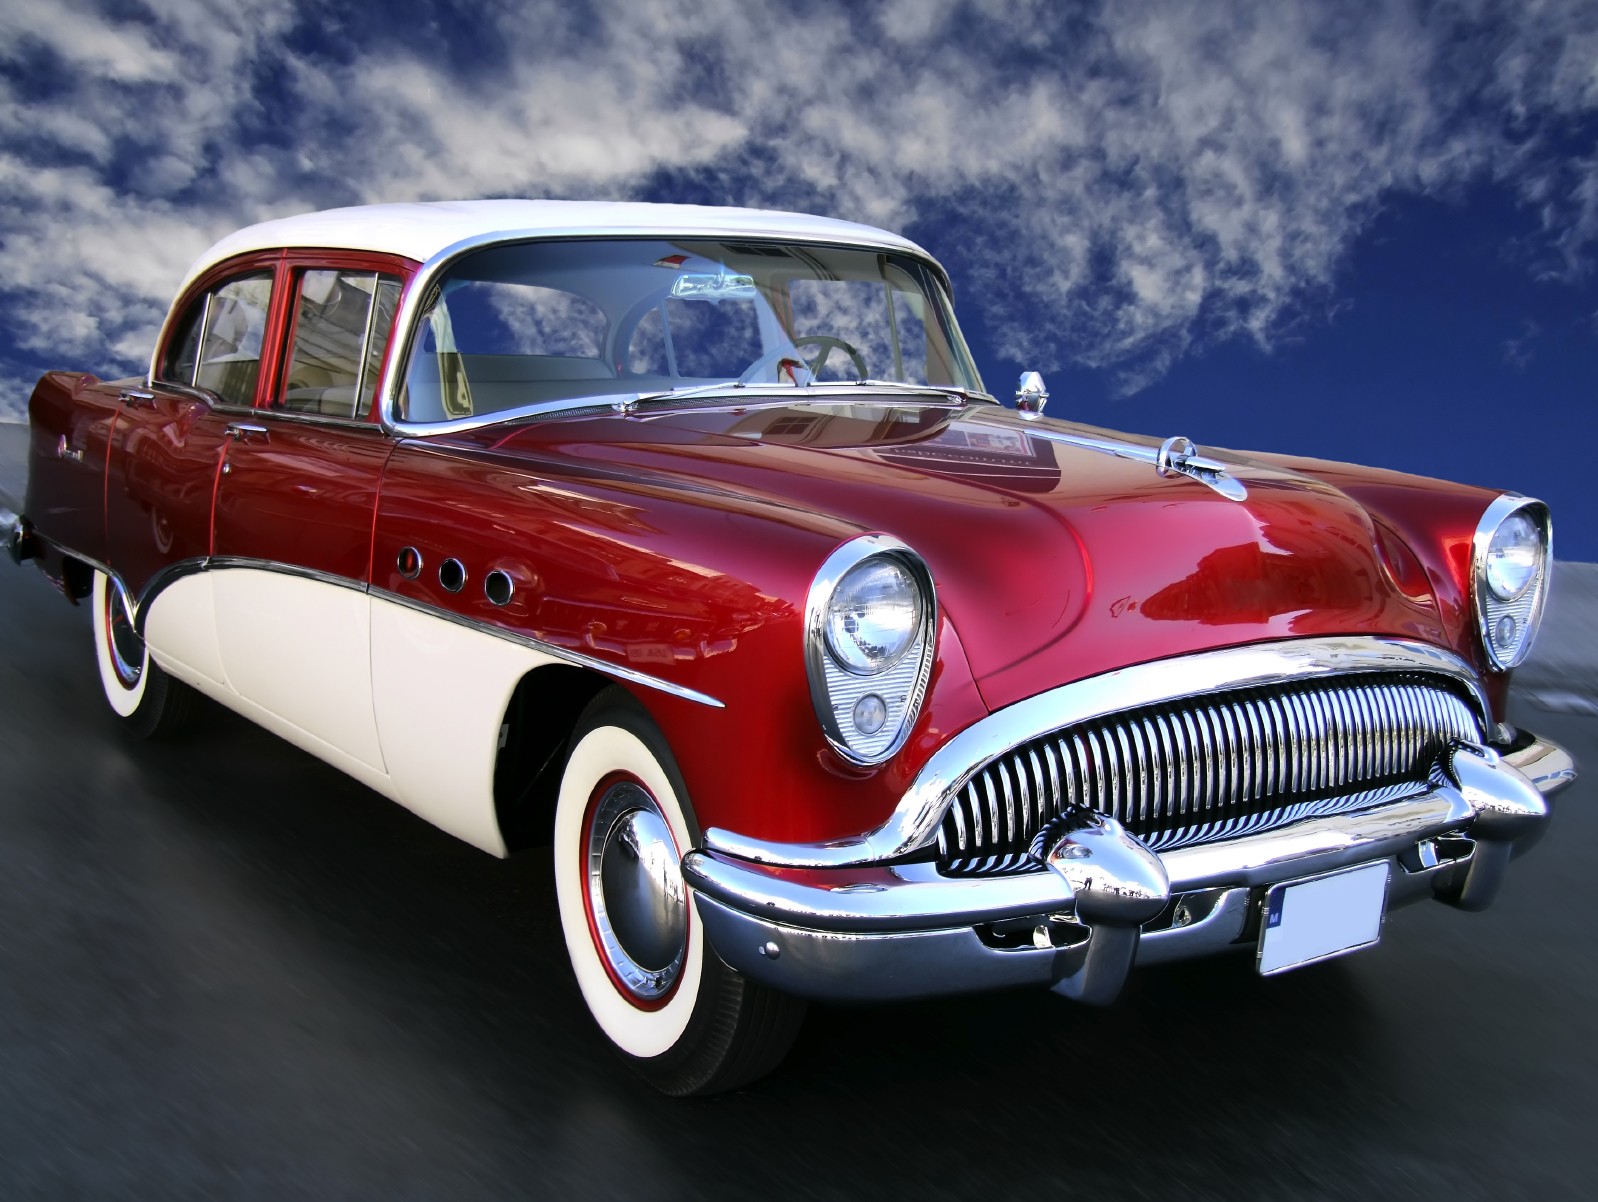
\includegraphics[width=\linewidth]{car.jpg} % ours reconstruction num.1	
	\end{subfigure}
	% second line
	\centering
	\begin{subfigure}[b]{0.225\linewidth}
		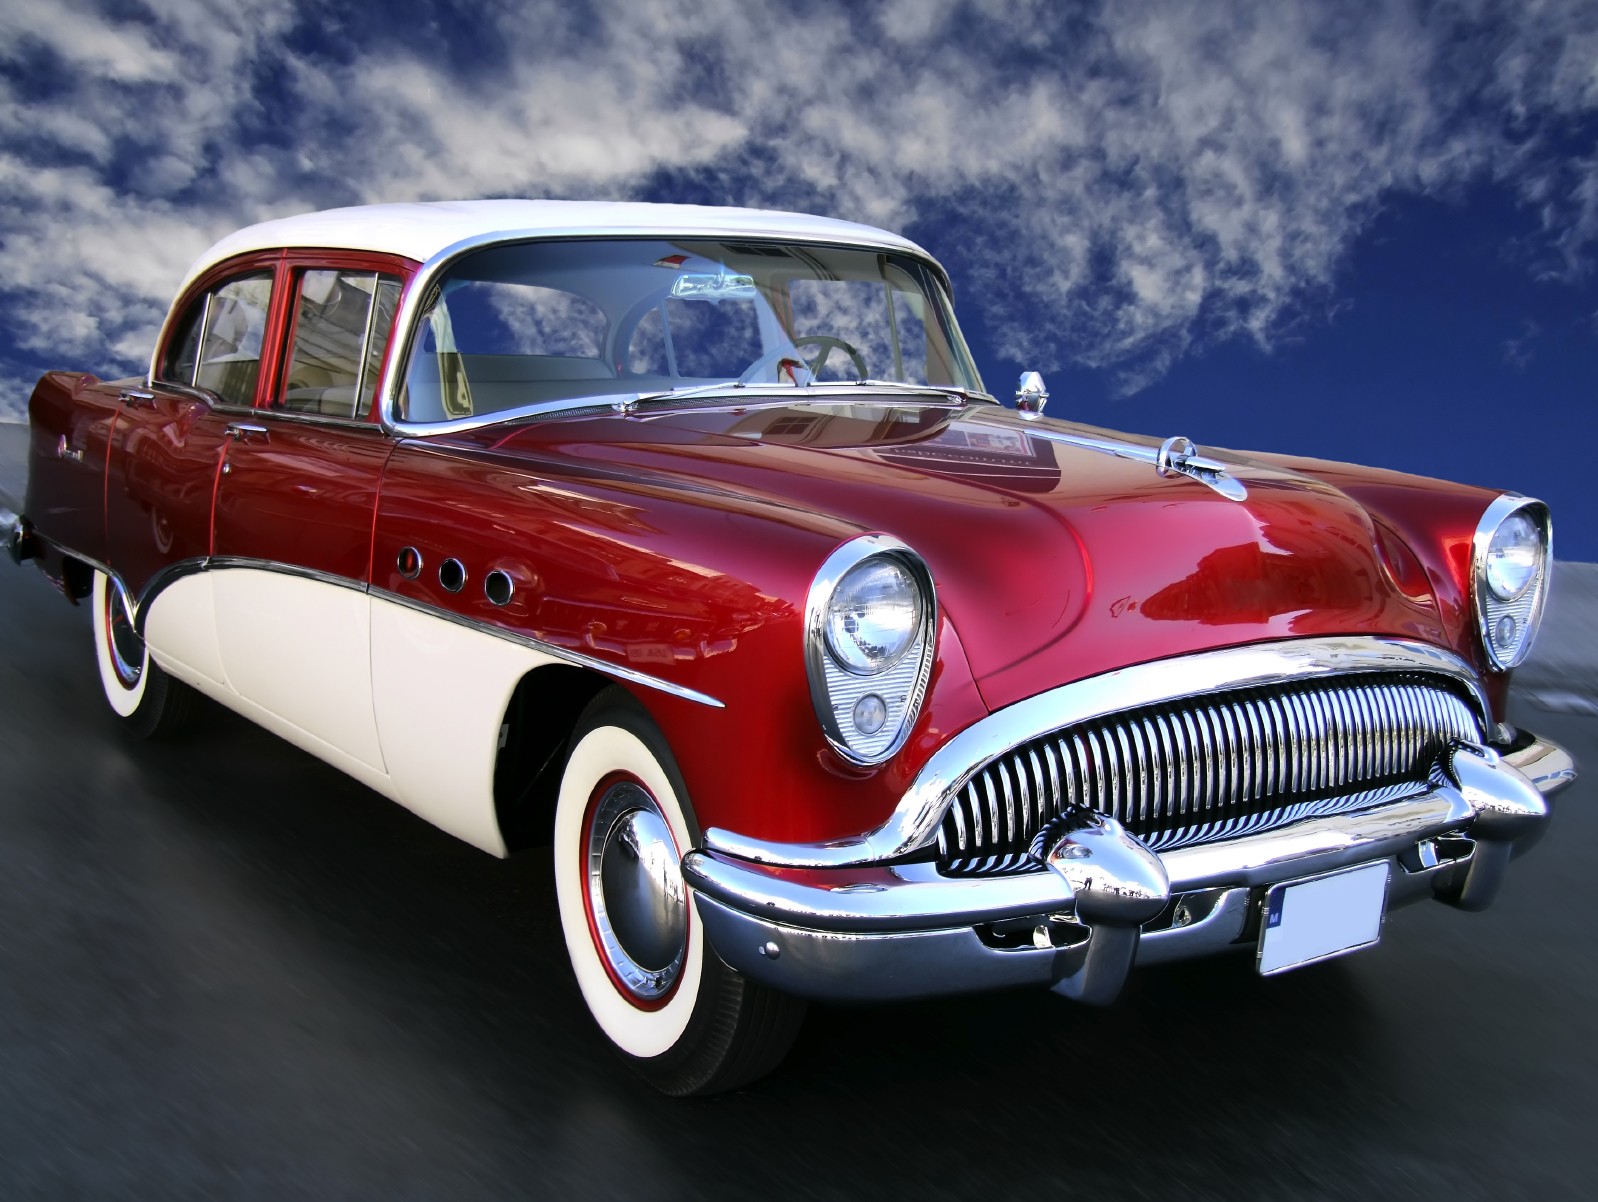
\includegraphics[width=\linewidth]{car.jpg} %style img num.2
	\end{subfigure}
	\begin{subfigure}[b]{0.225\linewidth}
		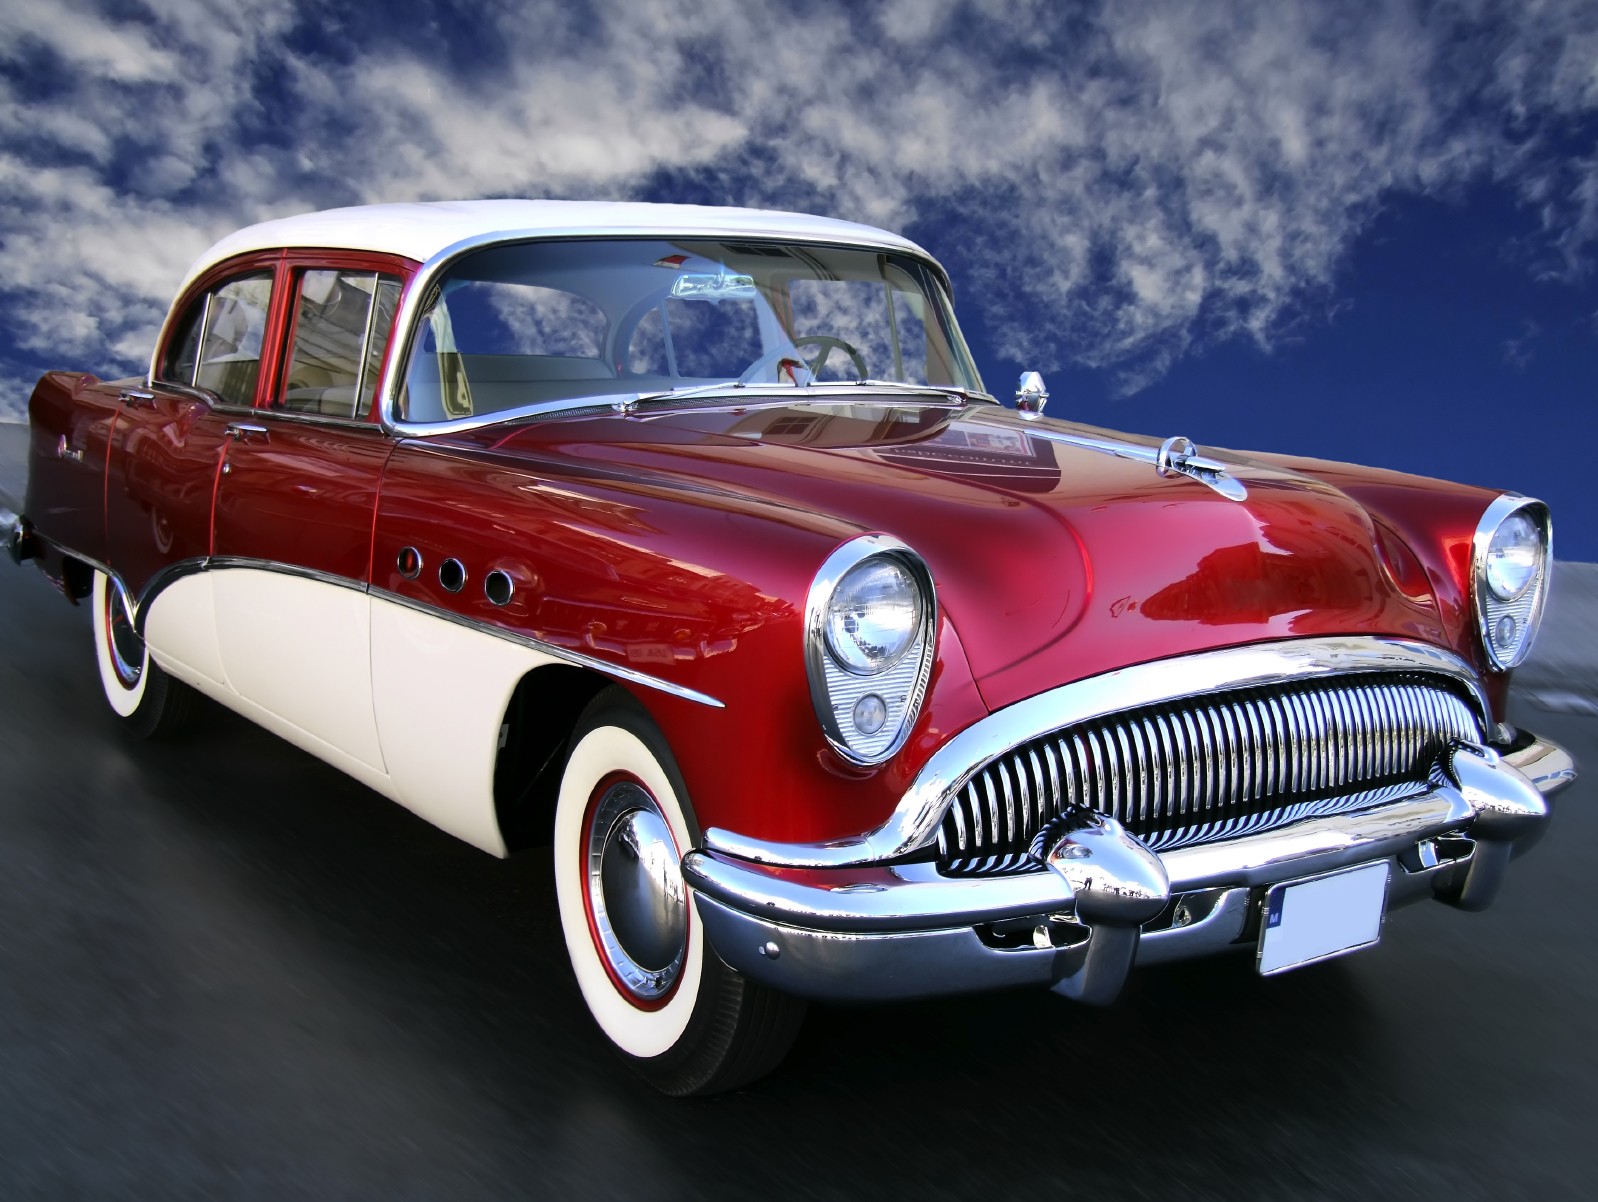
\includegraphics[width=\linewidth]{car.jpg} % content img num.2
	\end{subfigure}
	\begin{subfigure}[b]{0.225\linewidth}
		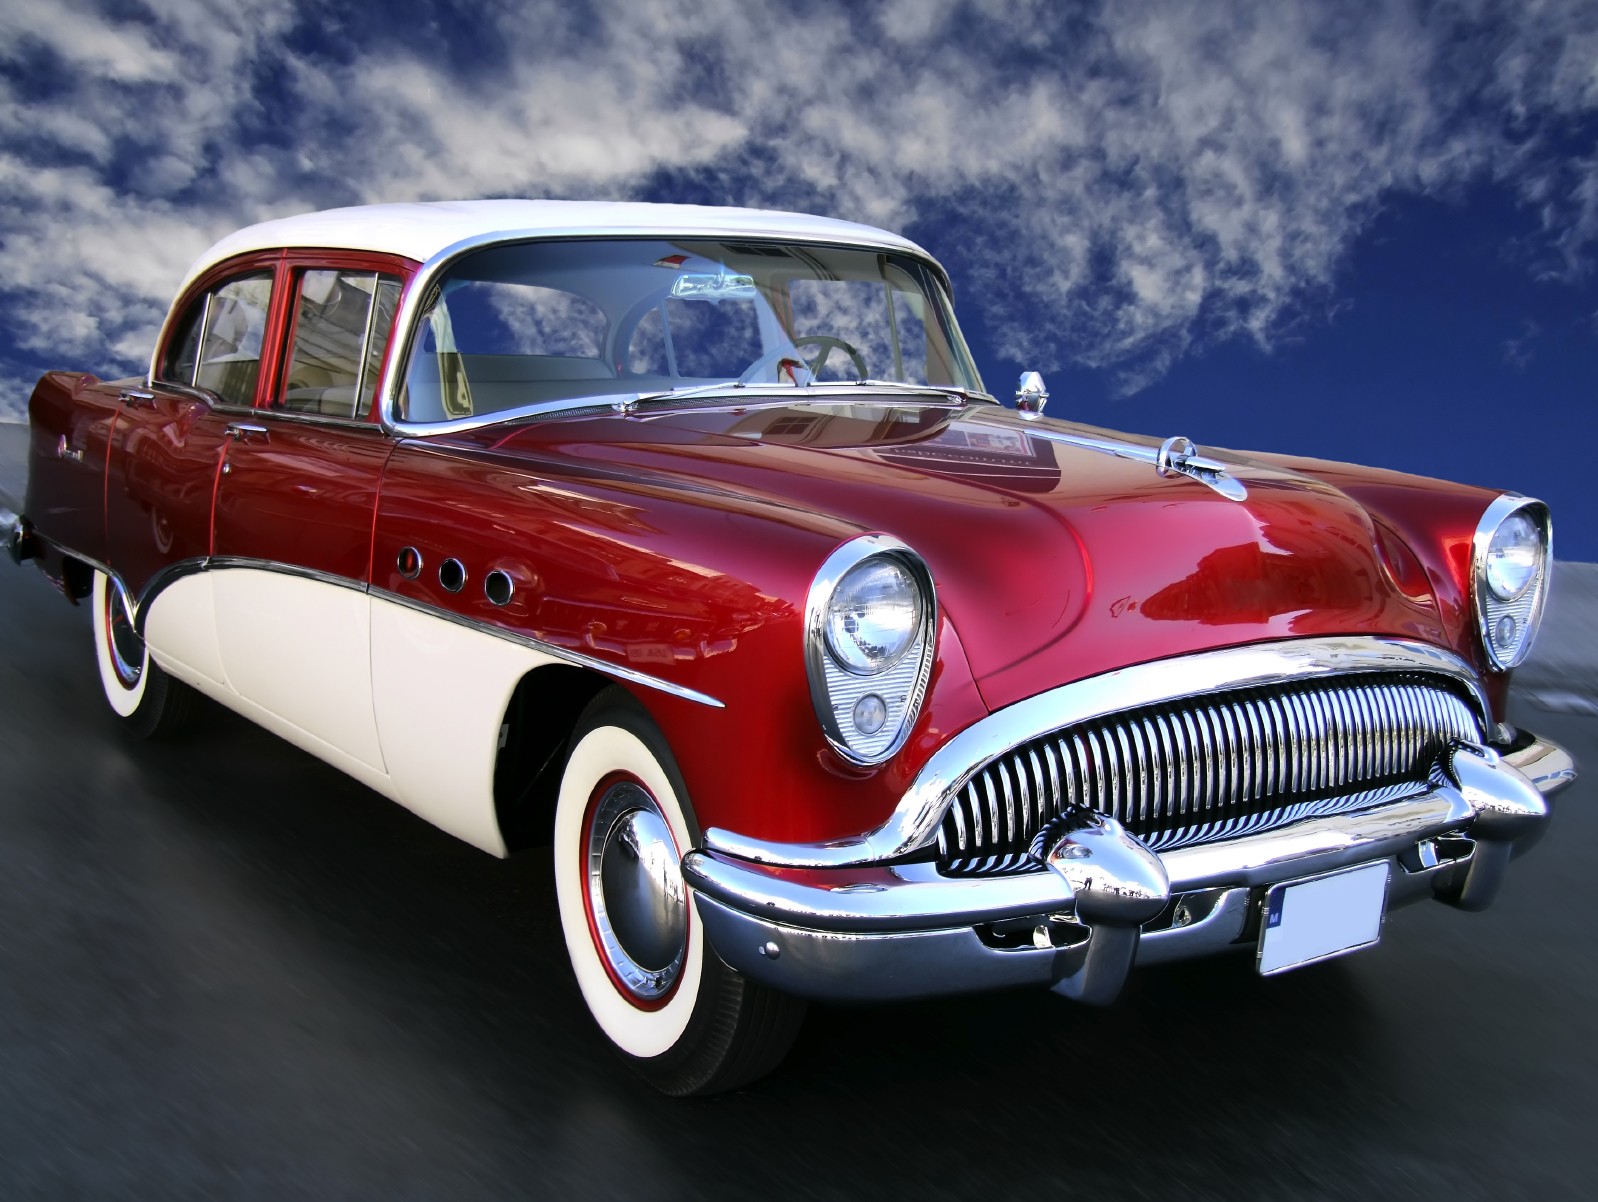
\includegraphics[width=\linewidth]{car.jpg} % theirs reconstruction num.2
	\end{subfigure}
	\begin{subfigure}[b]{0.225\linewidth}
		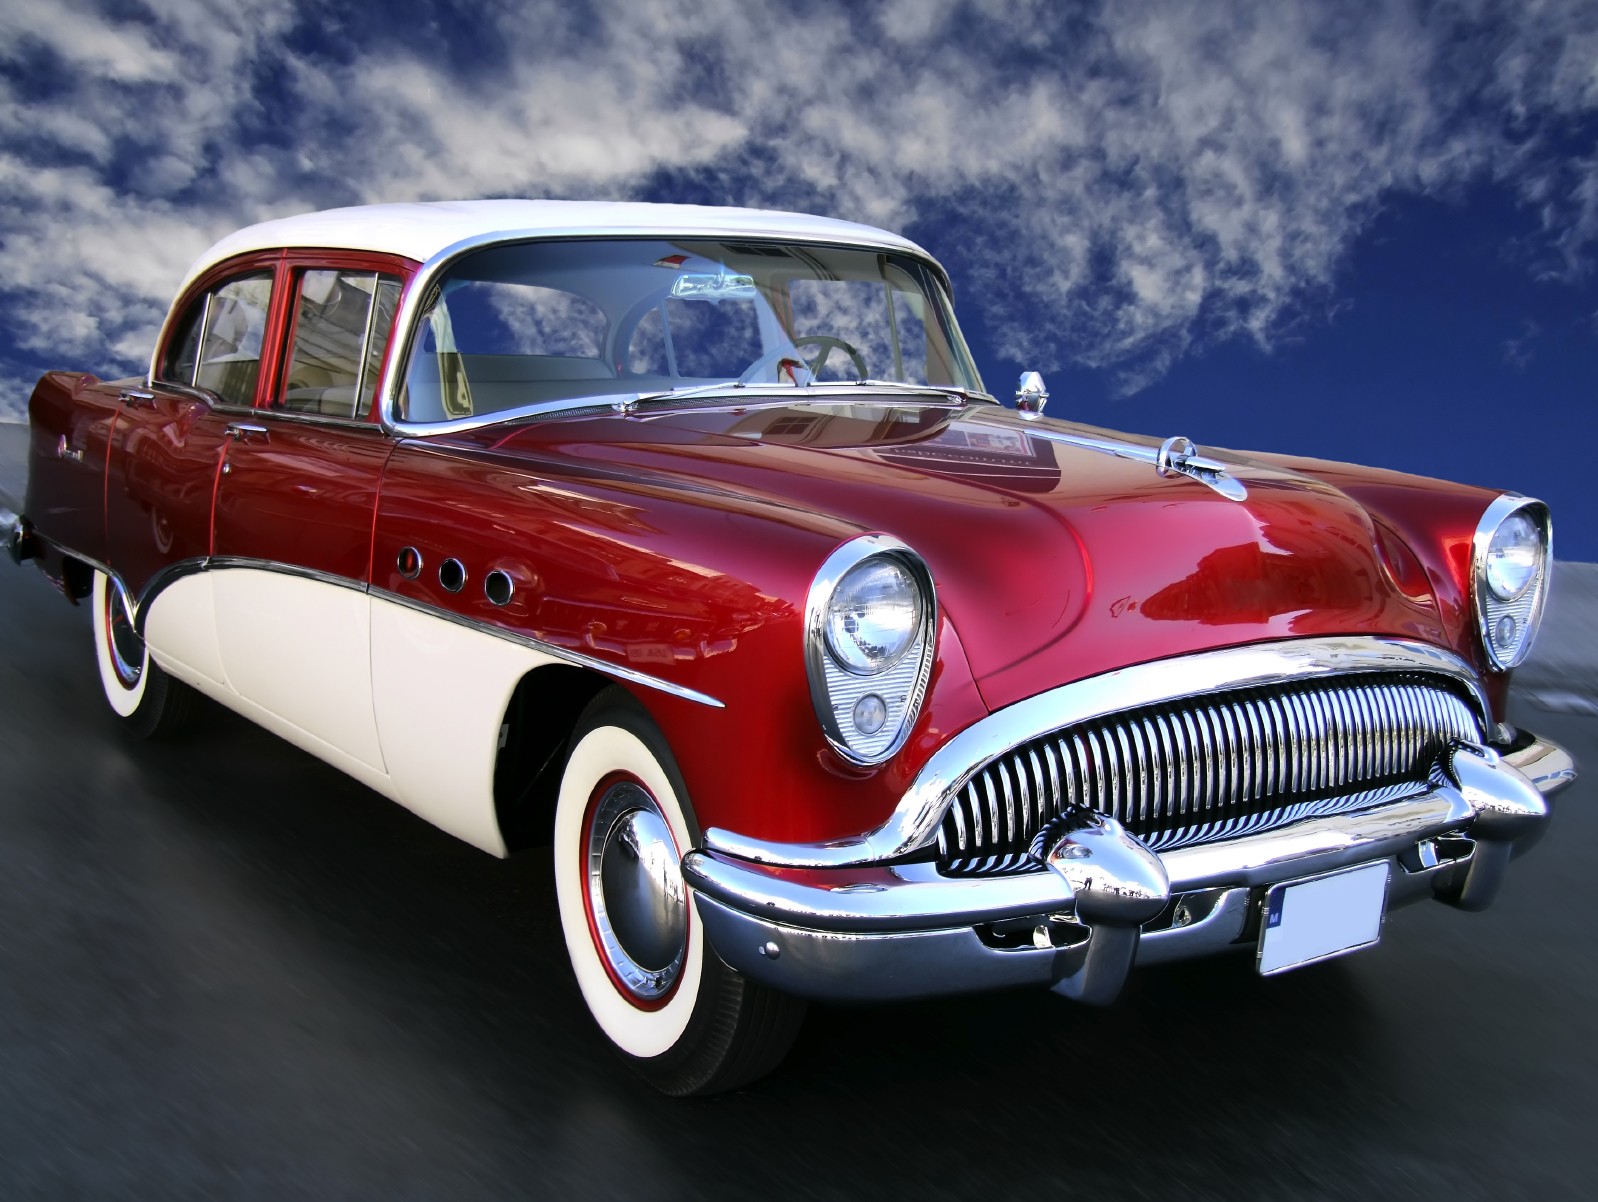
\includegraphics[width=\linewidth]{car.jpg} % ours reconstruction num.2
	\end{subfigure}
	% third line
	\centering
	\begin{subfigure}[b]{0.225\linewidth}
		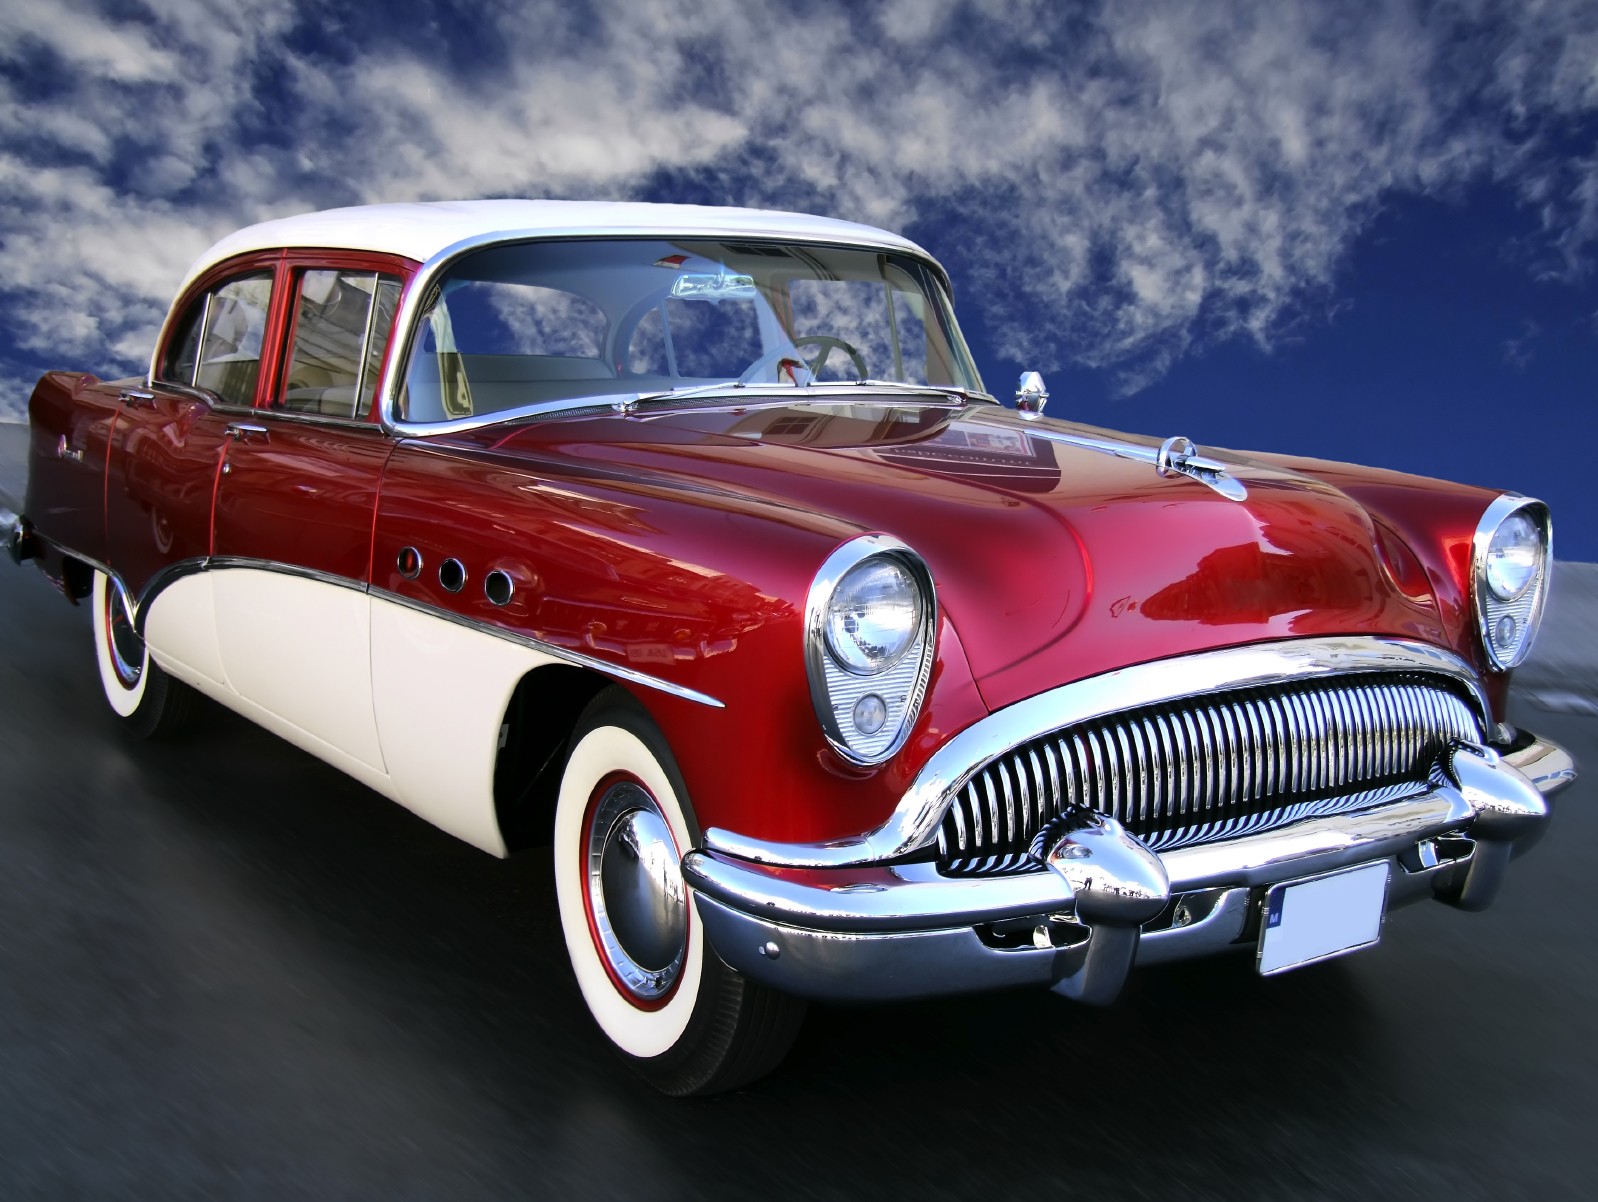
\includegraphics[width=\linewidth]{car.jpg} %style img num.3
	\end{subfigure}
	\begin{subfigure}[b]{0.225\linewidth}
		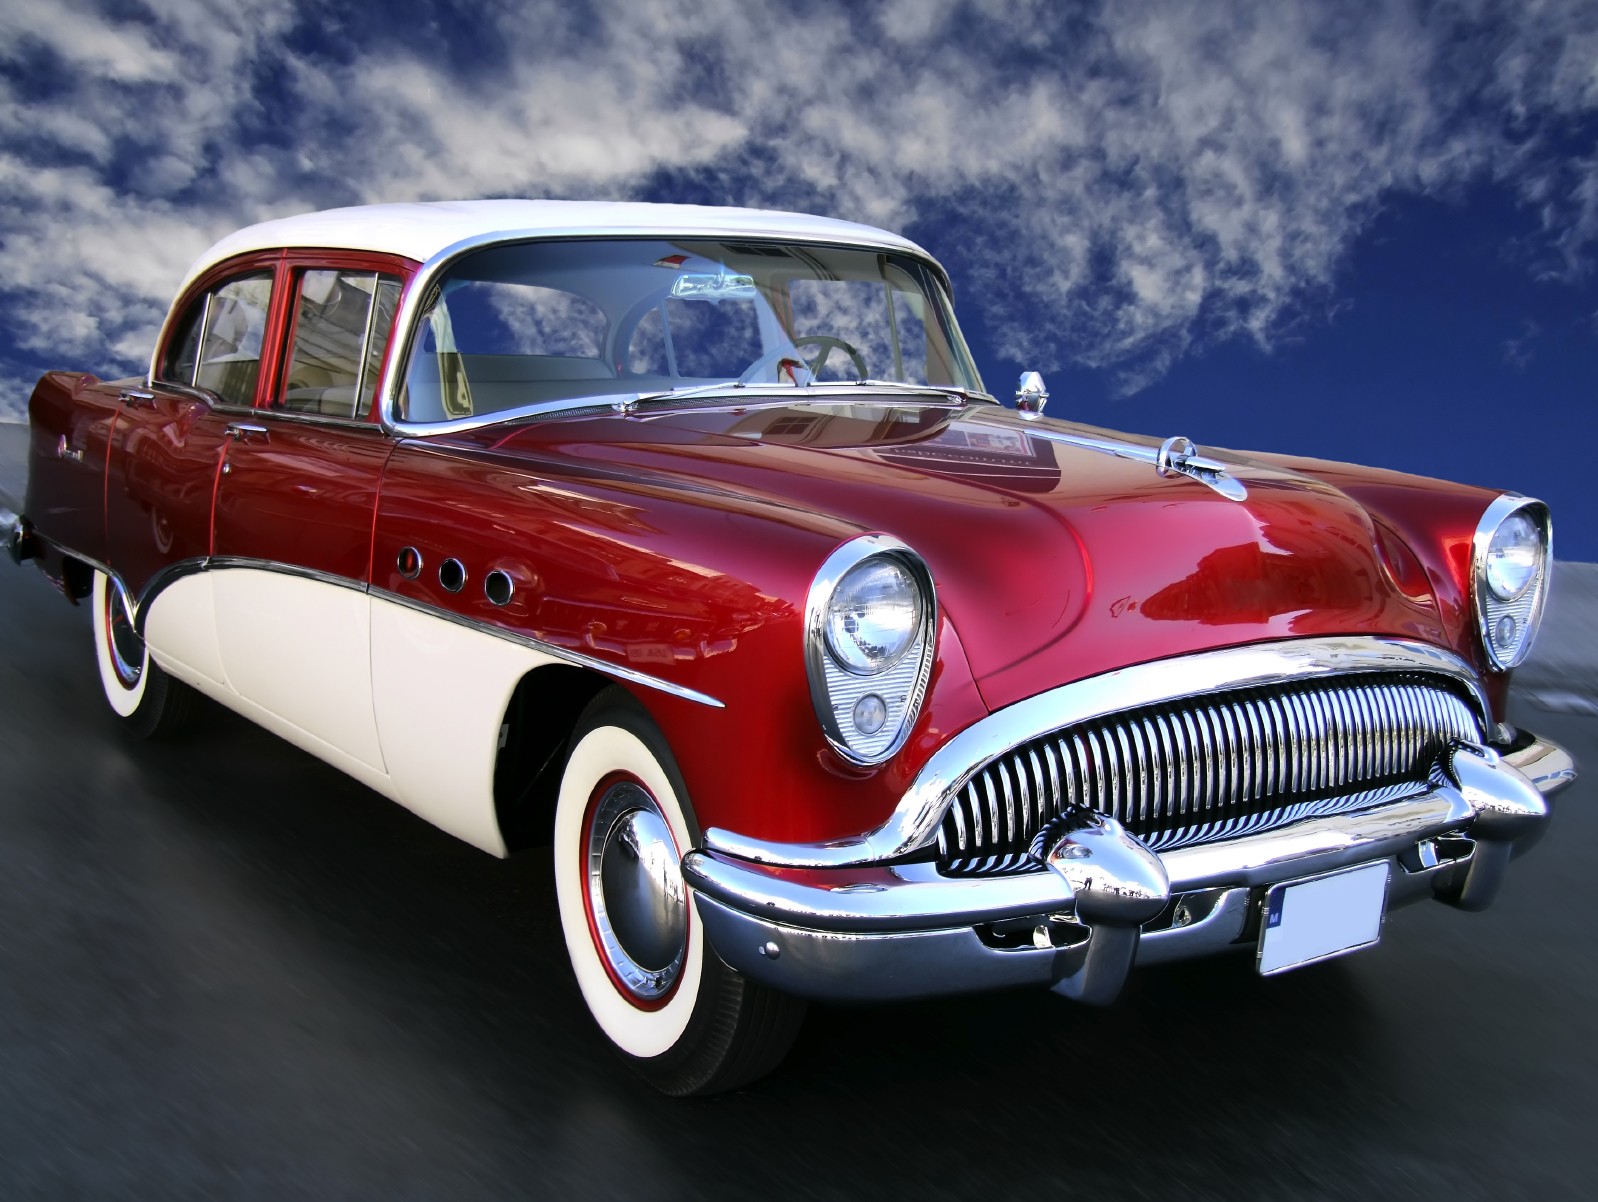
\includegraphics[width=\linewidth]{car.jpg} % content img num.3
	\end{subfigure}
	\begin{subfigure}[b]{0.225\linewidth}
		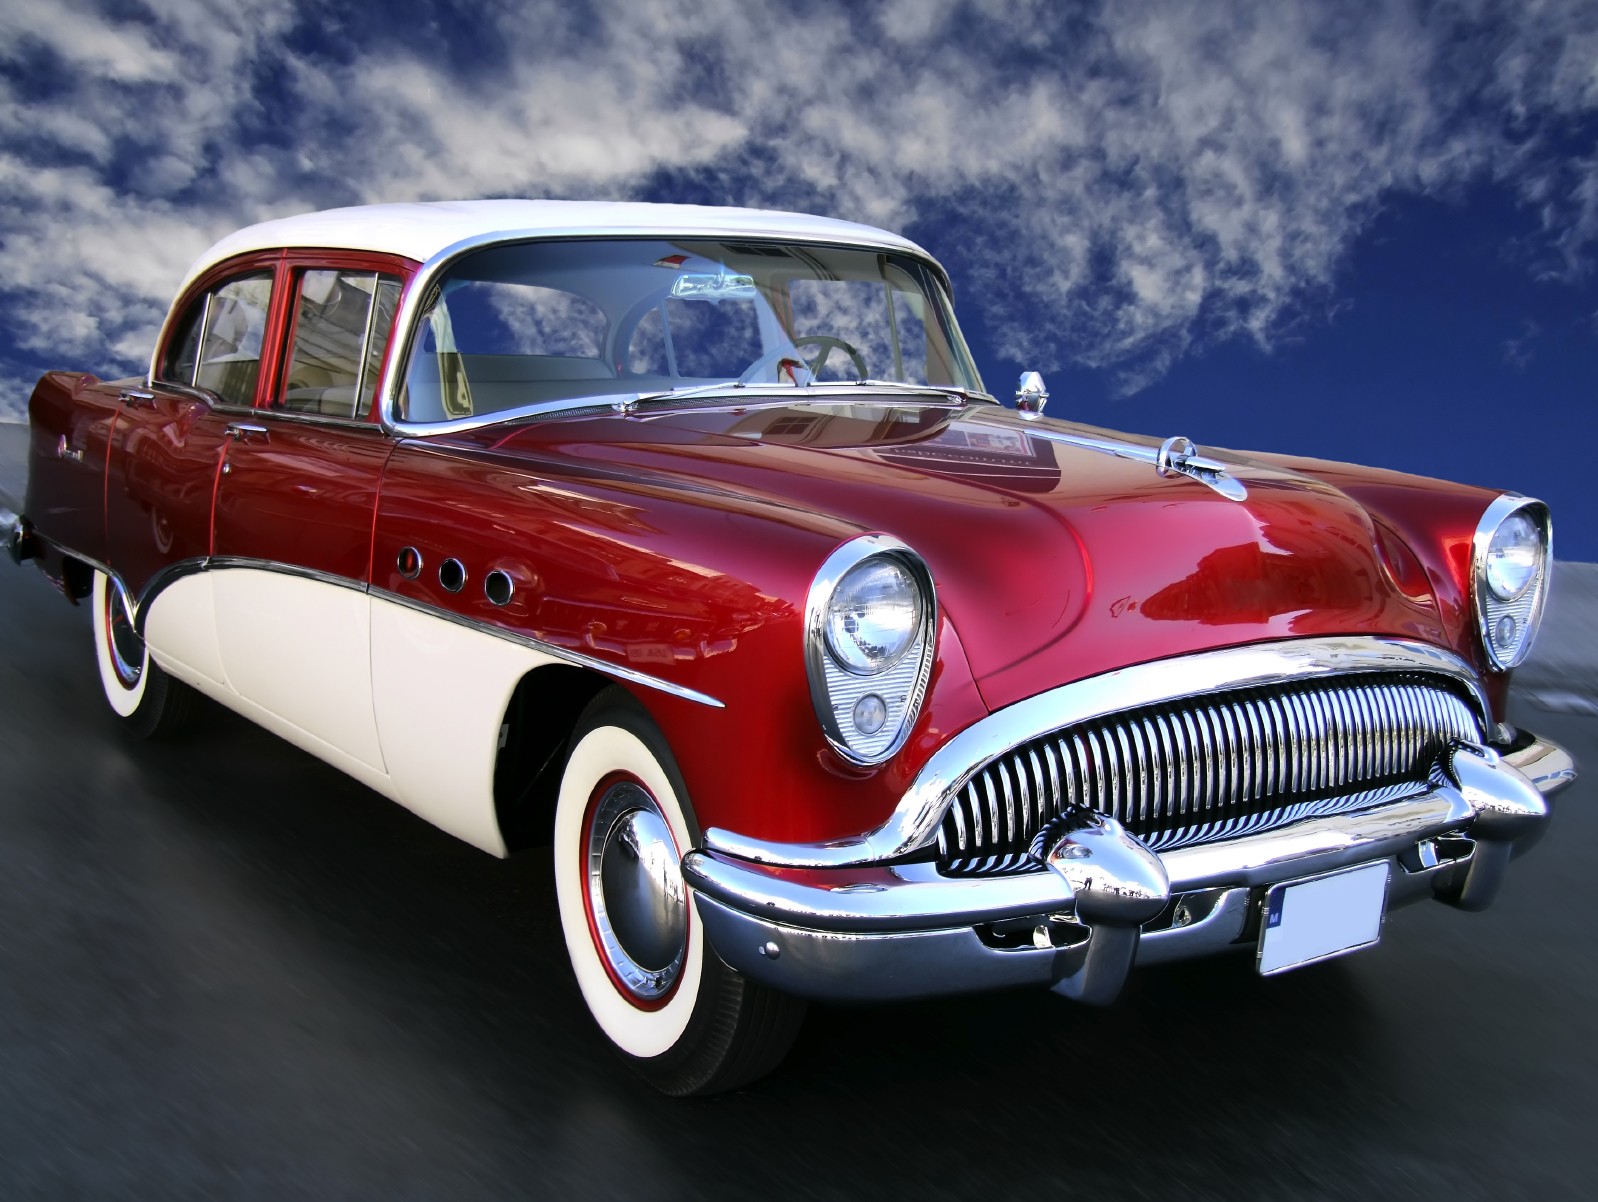
\includegraphics[width=\linewidth]{car.jpg} % theirs reconstruction num.3
	\end{subfigure}
	\begin{subfigure}[b]{0.225\linewidth}
		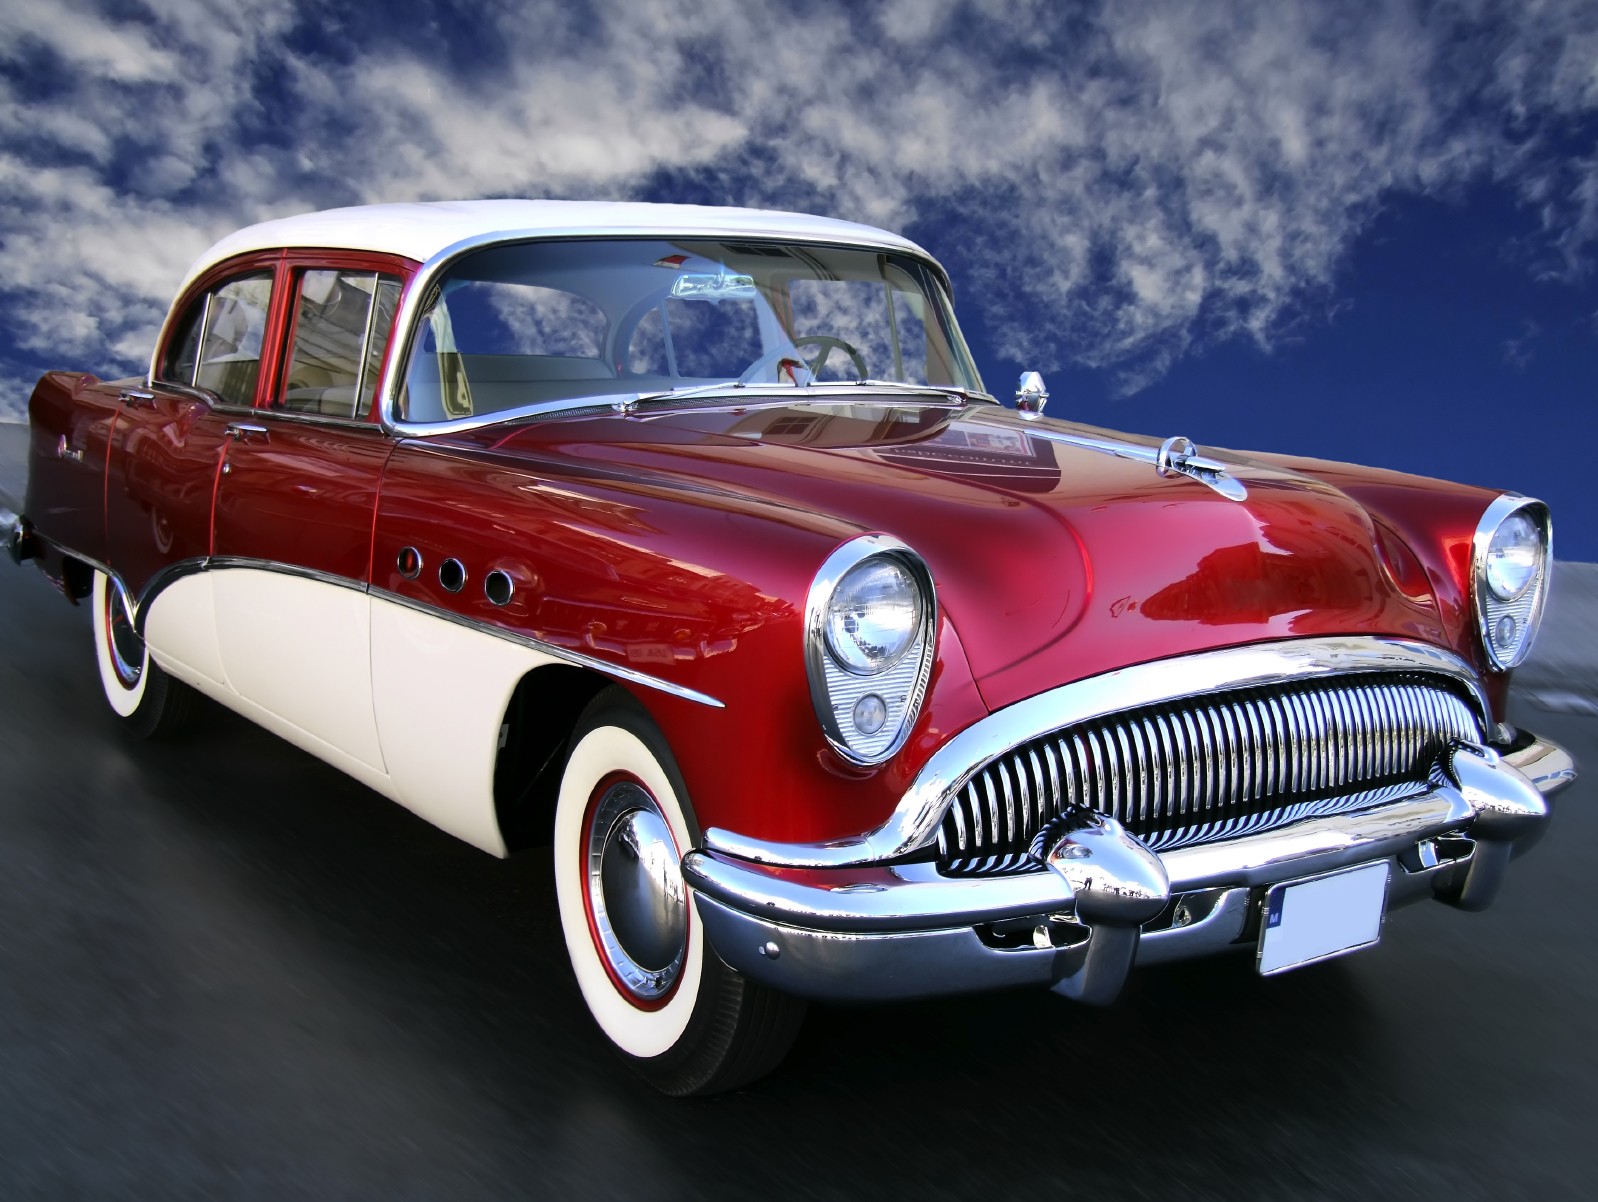
\includegraphics[width=\linewidth]{car.jpg} % ours reconstruction num.3
	\end{subfigure}
	% fourth line
	\centering
	\begin{subfigure}[b]{0.225\linewidth}
		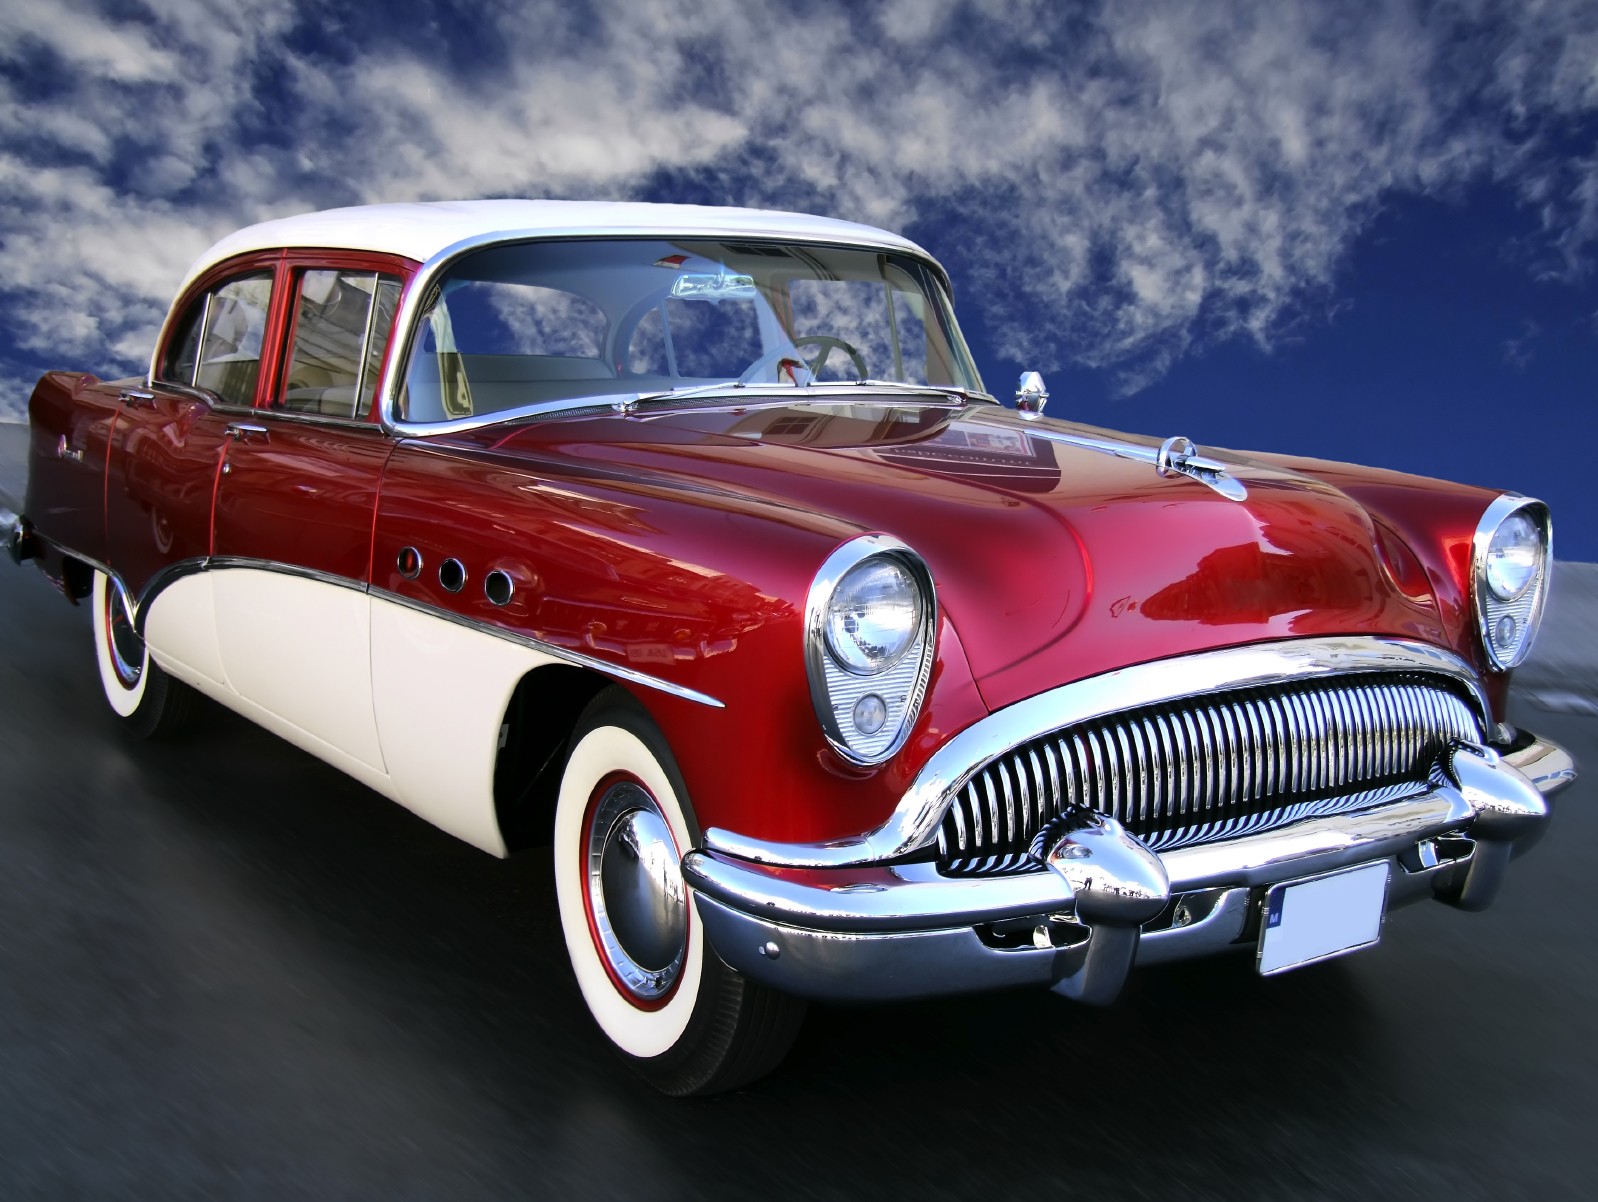
\includegraphics[width=\linewidth]{car.jpg} %style img num.4
	\end{subfigure}
	\begin{subfigure}[b]{0.225\linewidth}
		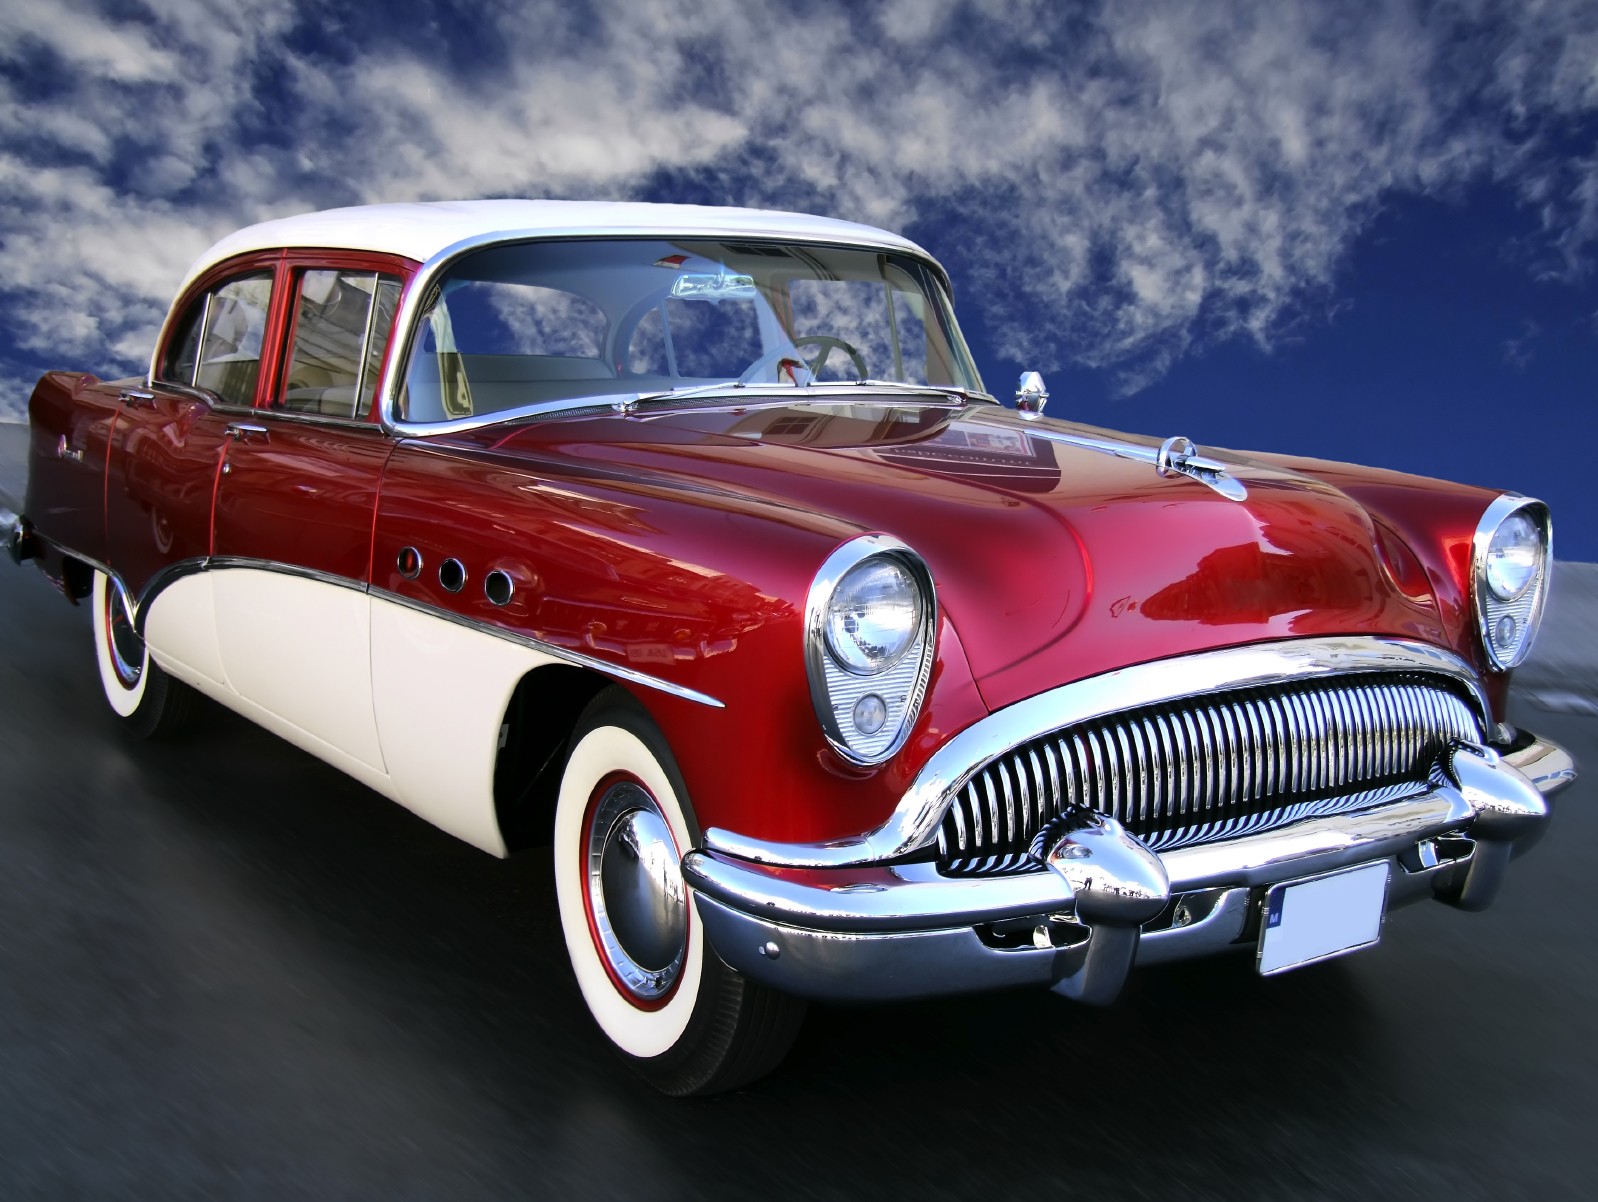
\includegraphics[width=\linewidth]{car.jpg} % content img num.4
	\end{subfigure}
	\begin{subfigure}[b]{0.225\linewidth}
		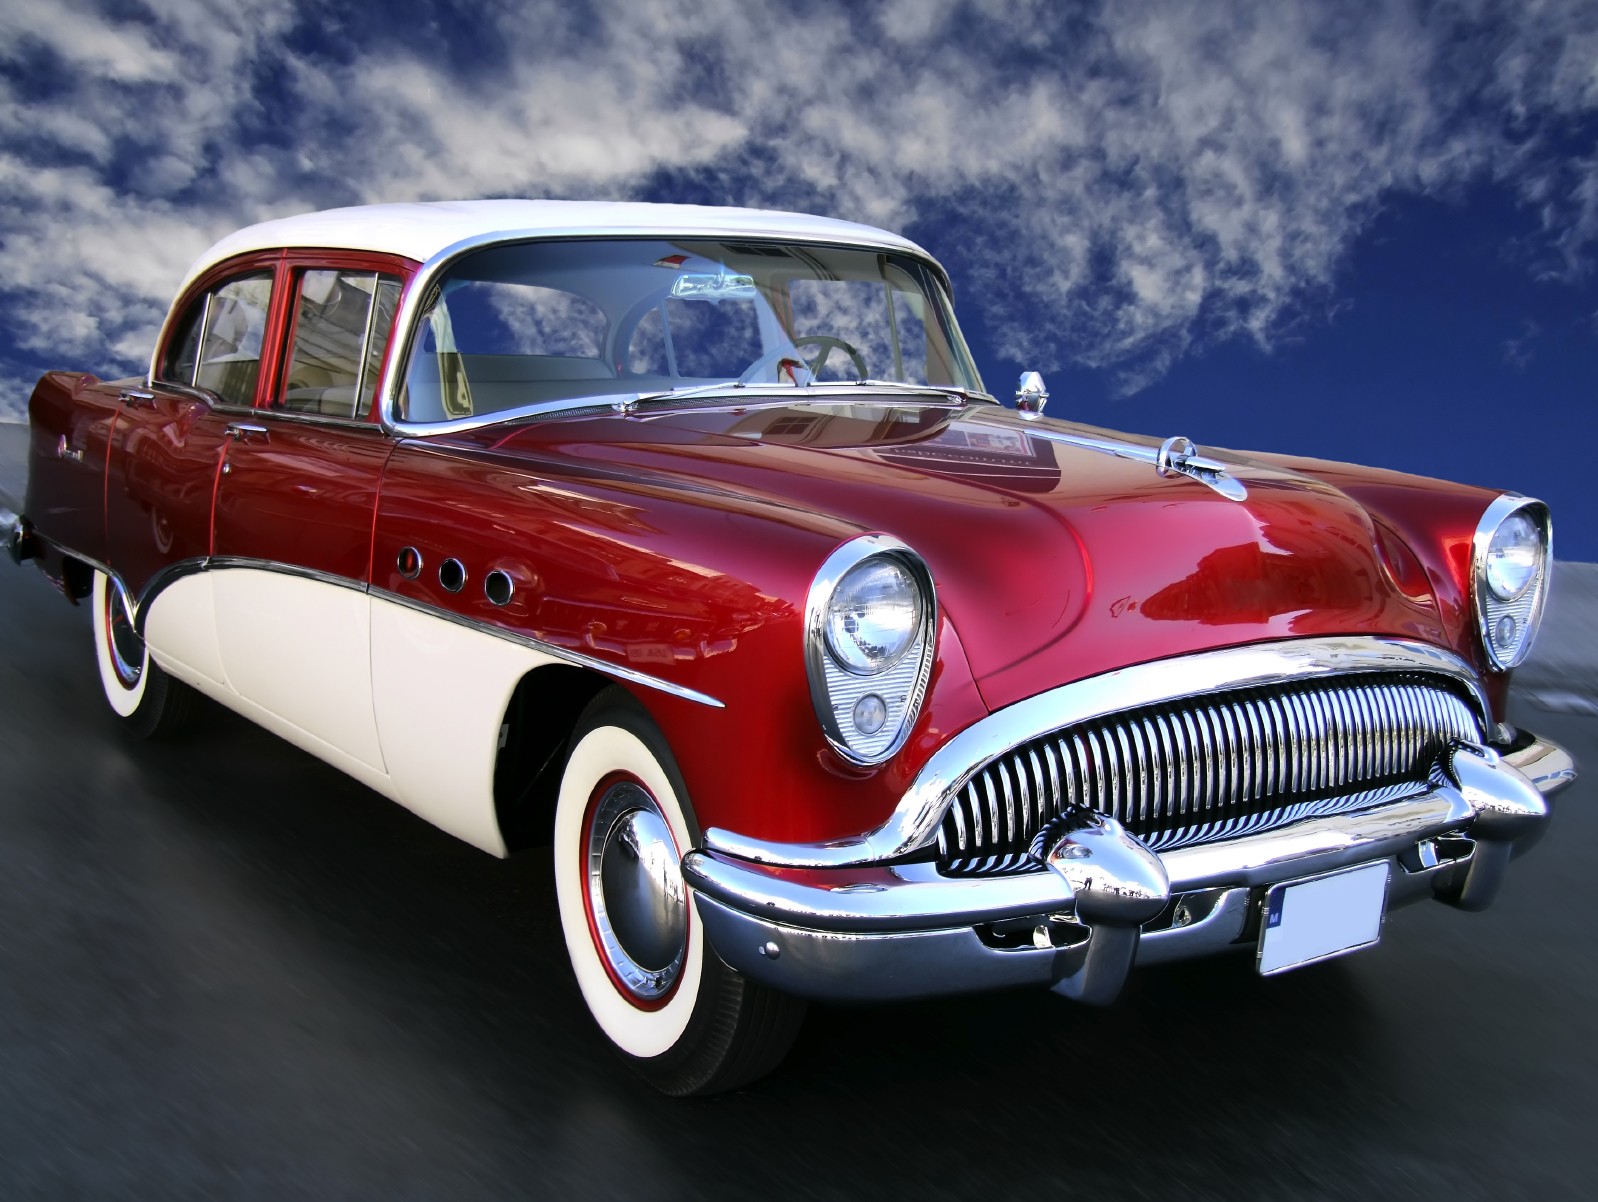
\includegraphics[width=\linewidth]{car.jpg} % theirs reconstruction num.4
	\end{subfigure}
	\begin{subfigure}[b]{0.225\linewidth}
		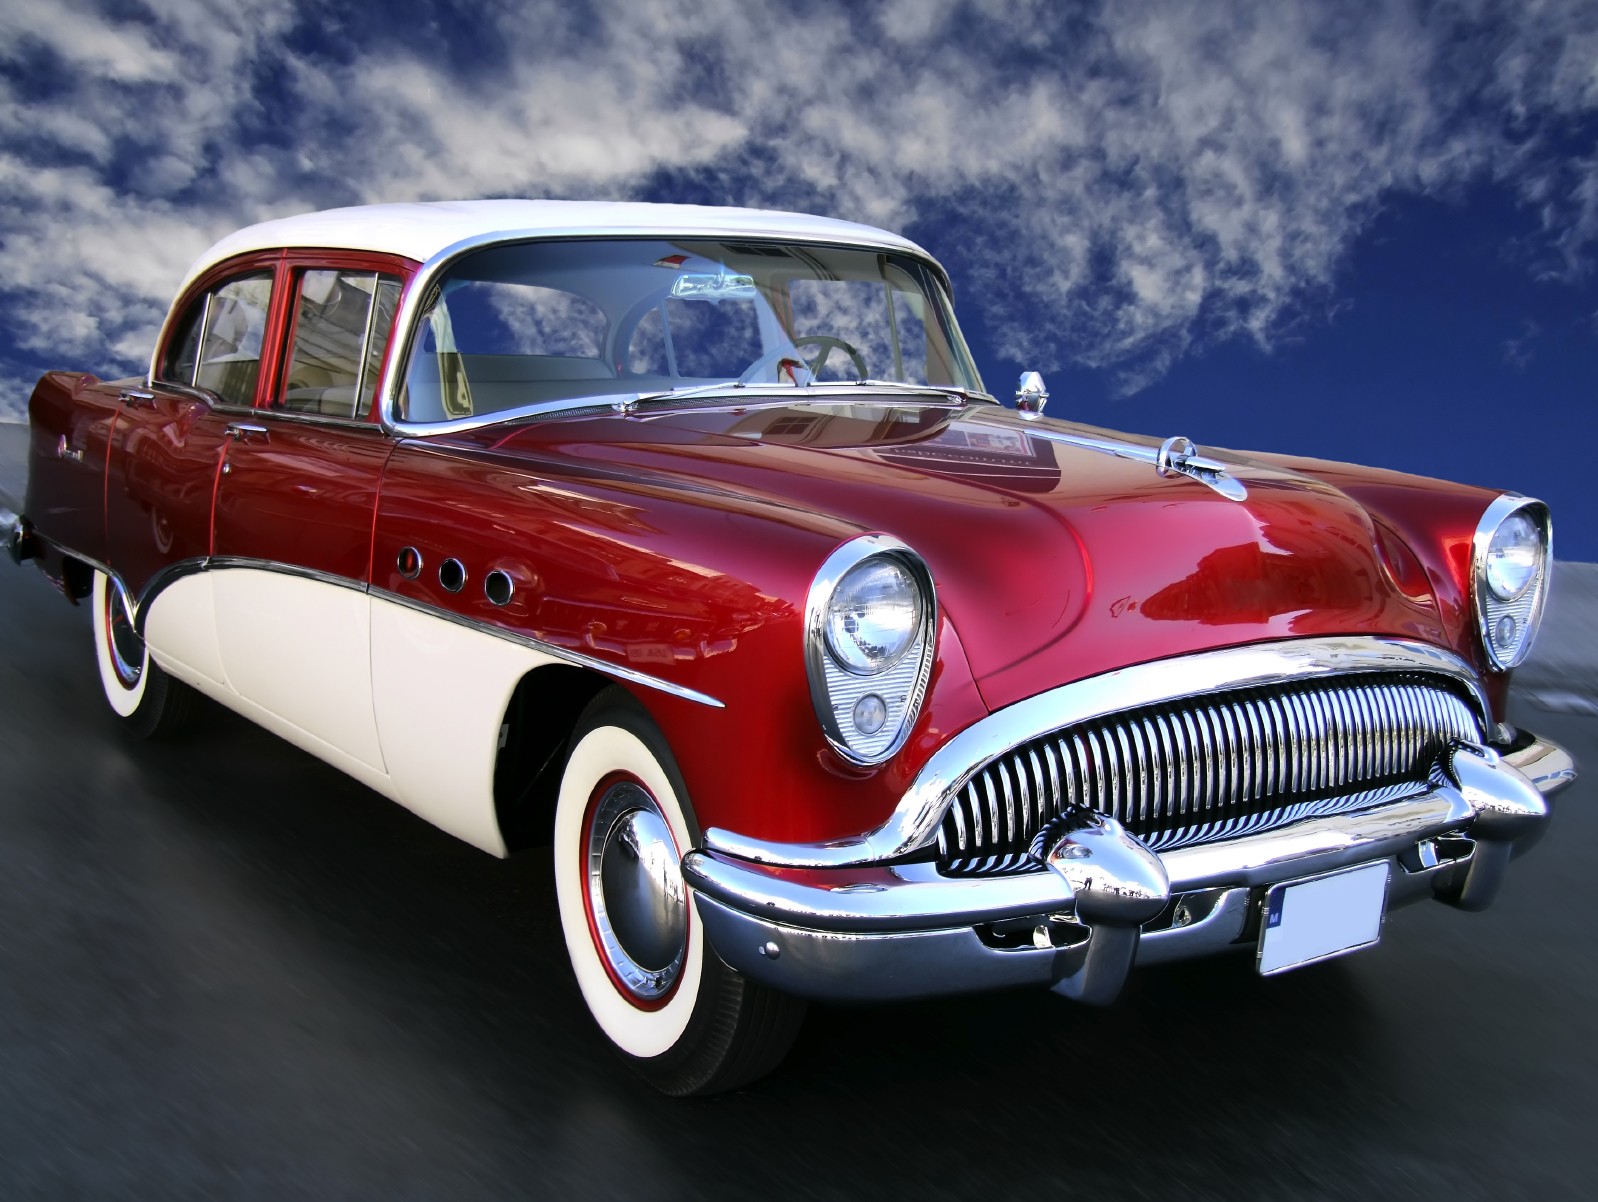
\includegraphics[width=\linewidth]{car.jpg} % ours reconstruction num.4
	\end{subfigure}
	% fifth line
	\centering
	\begin{subfigure}[b]{0.225\linewidth}
		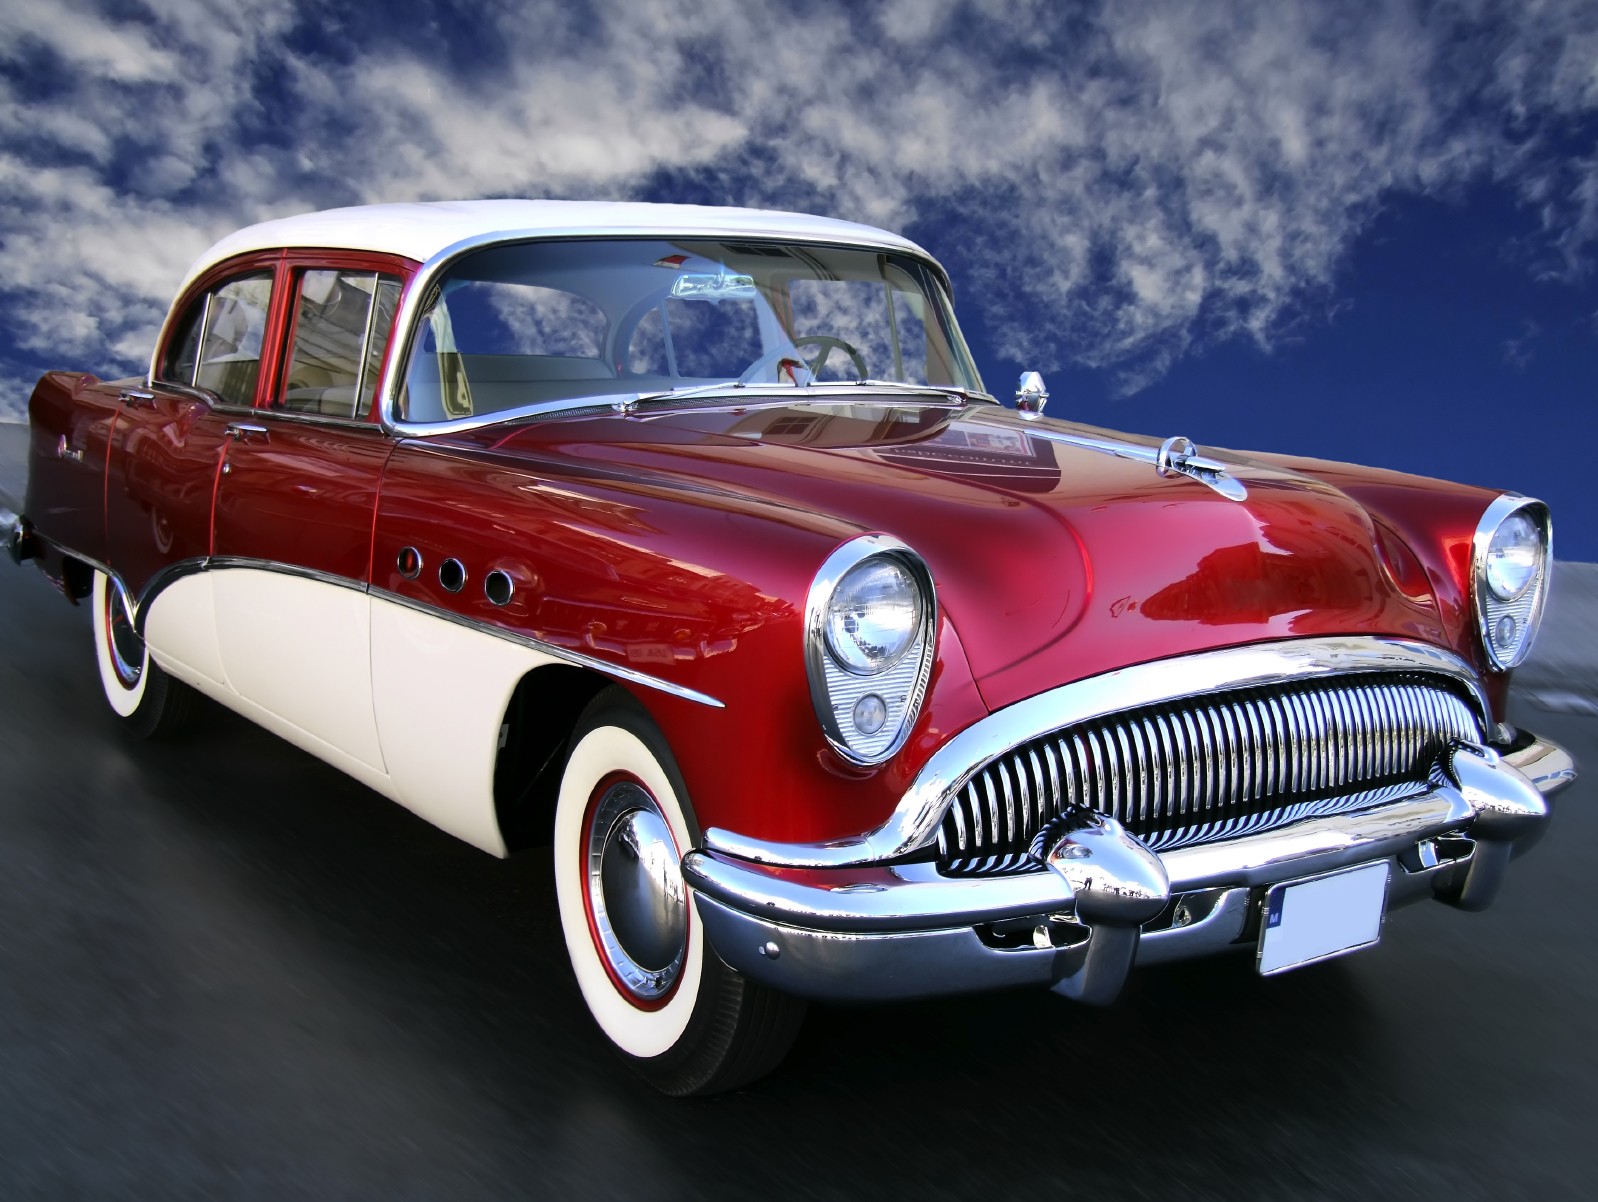
\includegraphics[width=\linewidth]{car.jpg} %style img num.5
		\caption{Style}
	\end{subfigure}
	\begin{subfigure}[b]{0.225\linewidth}
		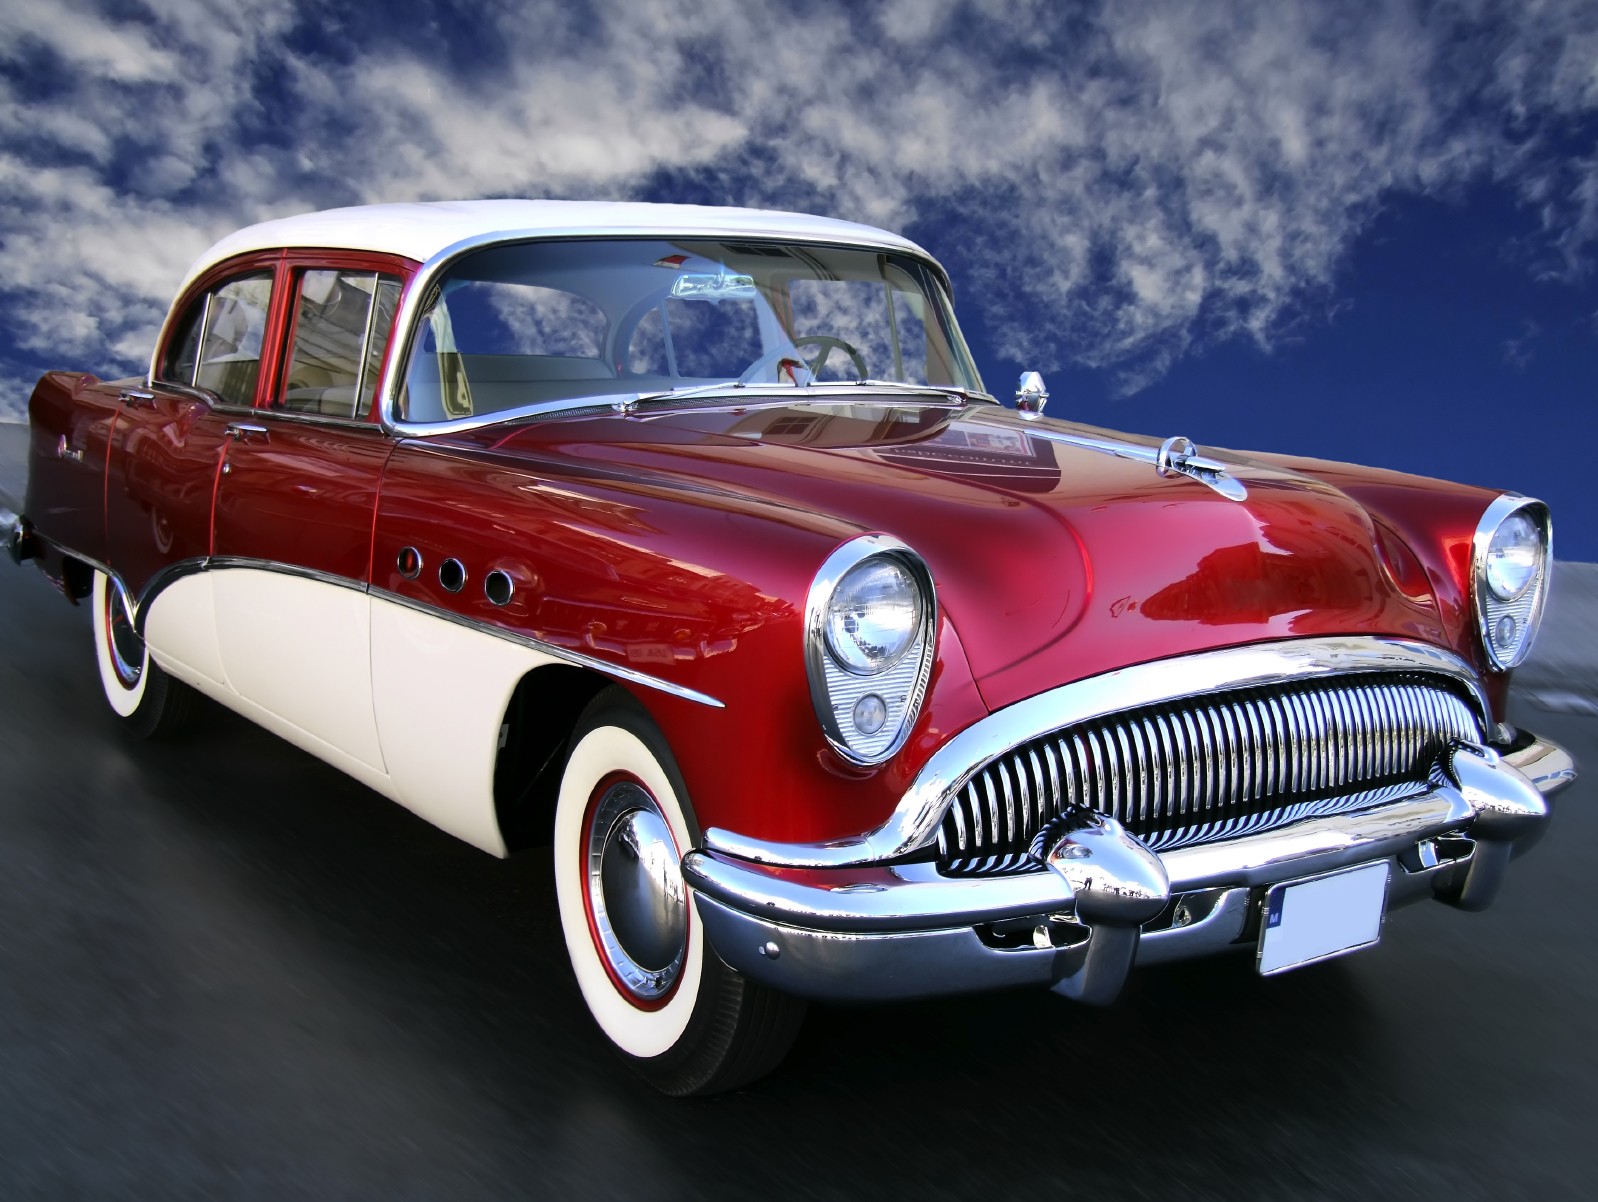
\includegraphics[width=\linewidth]{car.jpg} % content img num.5
		\caption{Content}
	\end{subfigure}
	\begin{subfigure}[b]{0.225\linewidth}
		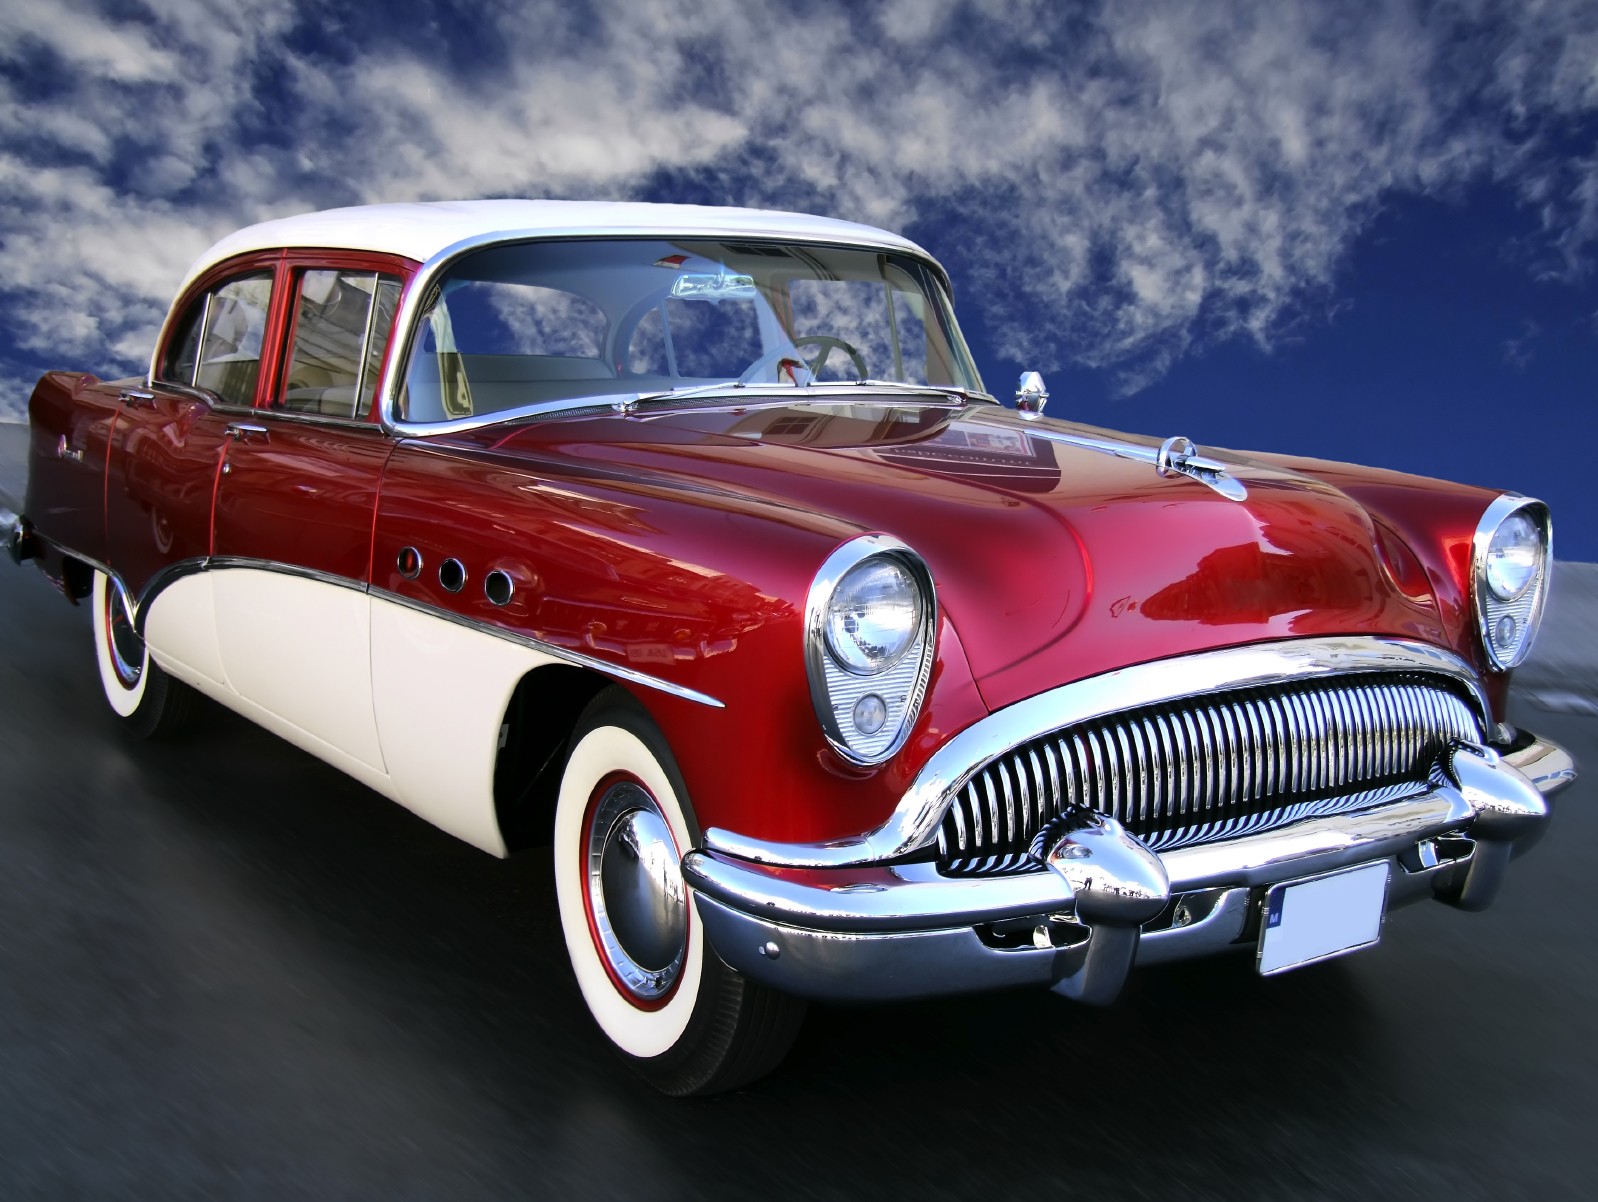
\includegraphics[width=\linewidth]{car.jpg} % theirs reconstruction num.5
		\caption{Li et al. \cite{bib11}}
	\end{subfigure}
	\begin{subfigure}[b]{0.225\linewidth}
		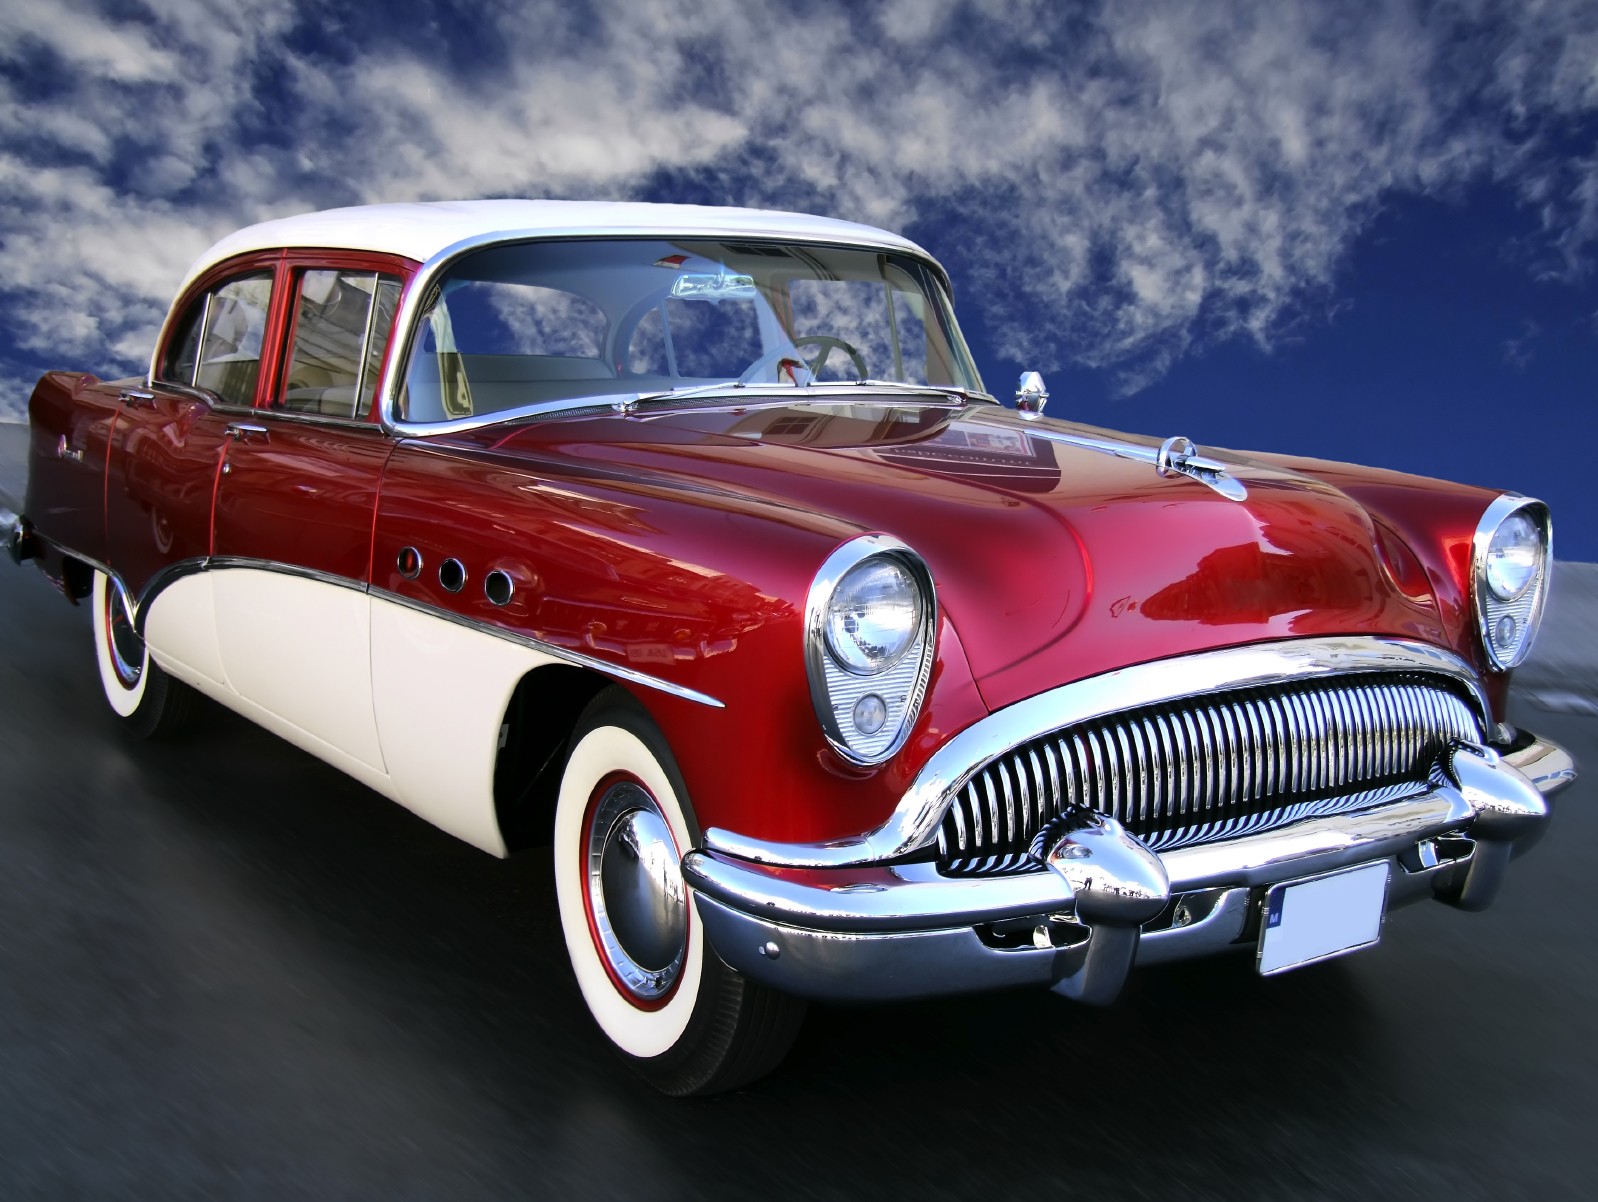
\includegraphics[width=\linewidth]{car.jpg} % ours reconstruction num.5
		\caption{Our implementation}
	\end{subfigure}
	\caption{Results from different style transfer methods. We used the same encoder as \cite{bib11} but trained from scratch 5 different decoder architectures and we implemented WCT algorithm. Style weight $\alpha=0.5$}
	\label{fig:style_transfer}
\end{figure}
% Boost  %
\begin{flushleft}
	\textbf{4.4 Stylization boosting algorithm}\newline
\end{flushleft}
\begin{figure}[h!]
	% first line
	\centering
	\begin{subfigure}[b]{0.225\linewidth}
		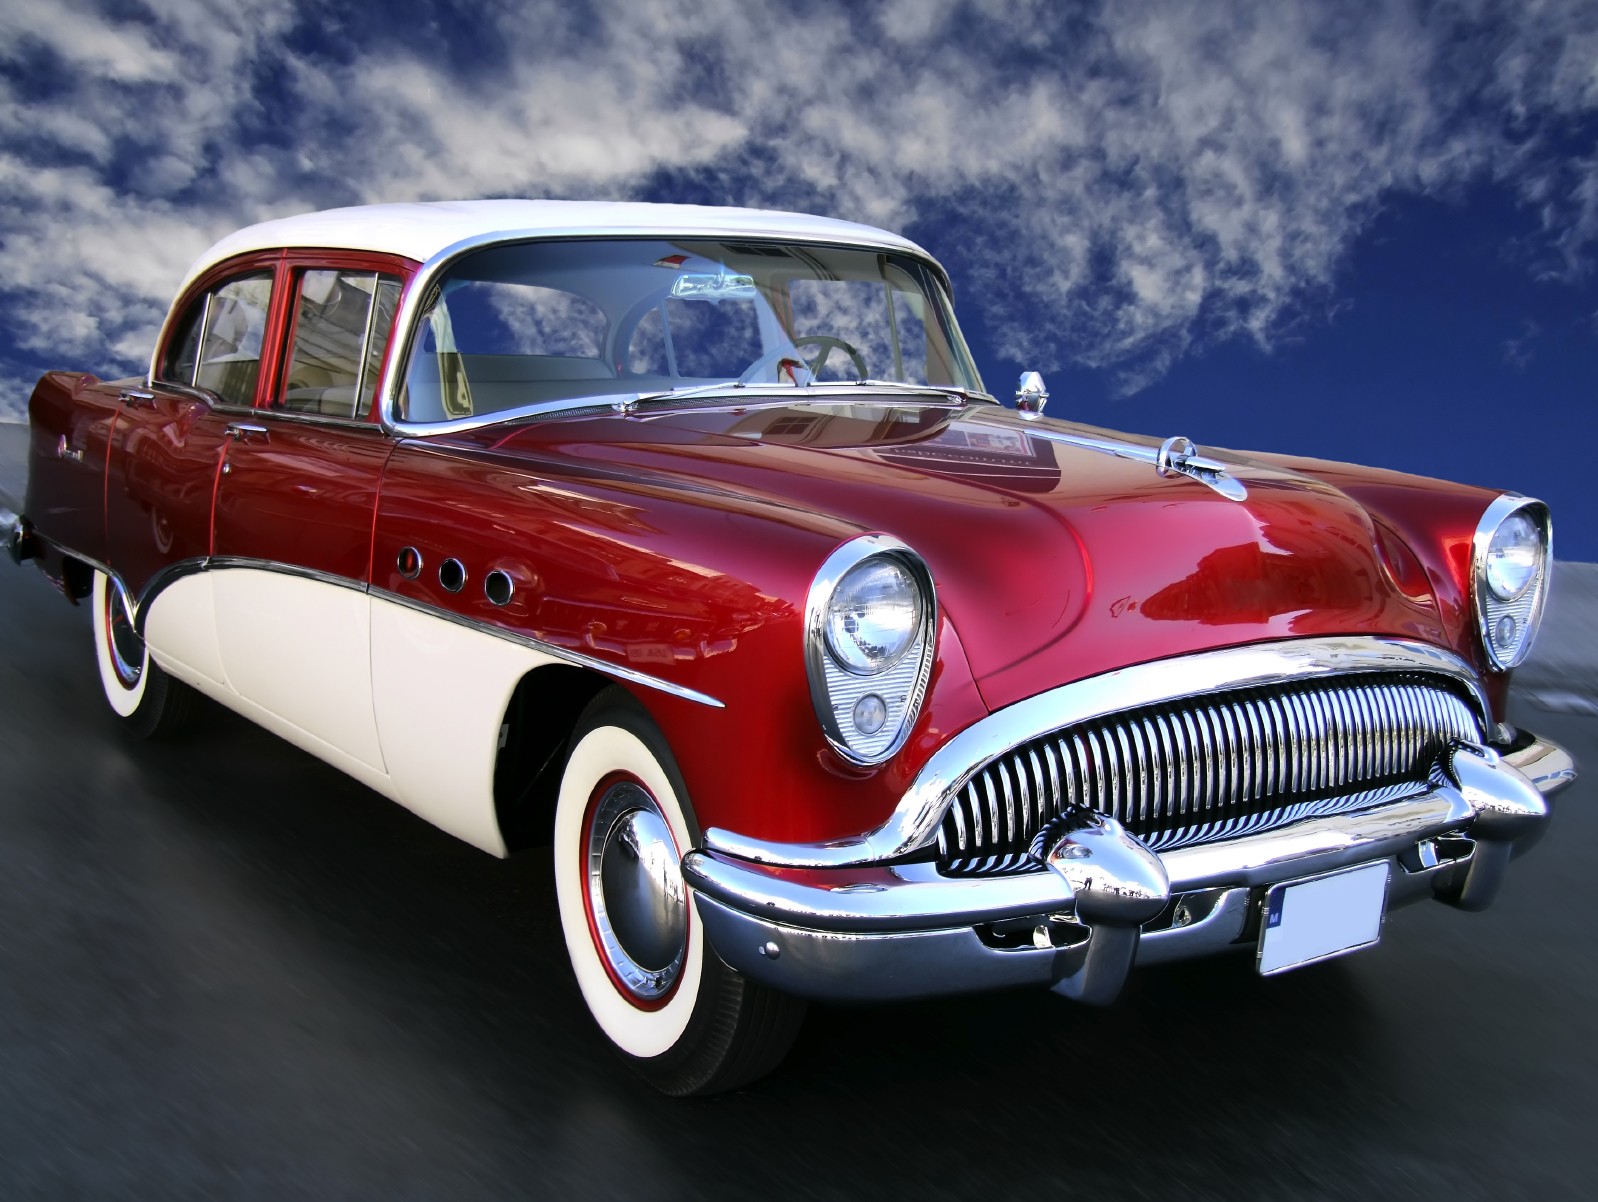
\includegraphics[width=\linewidth]{car.jpg} %style img num.1
	\end{subfigure}
	\begin{subfigure}[b]{0.225\linewidth}
		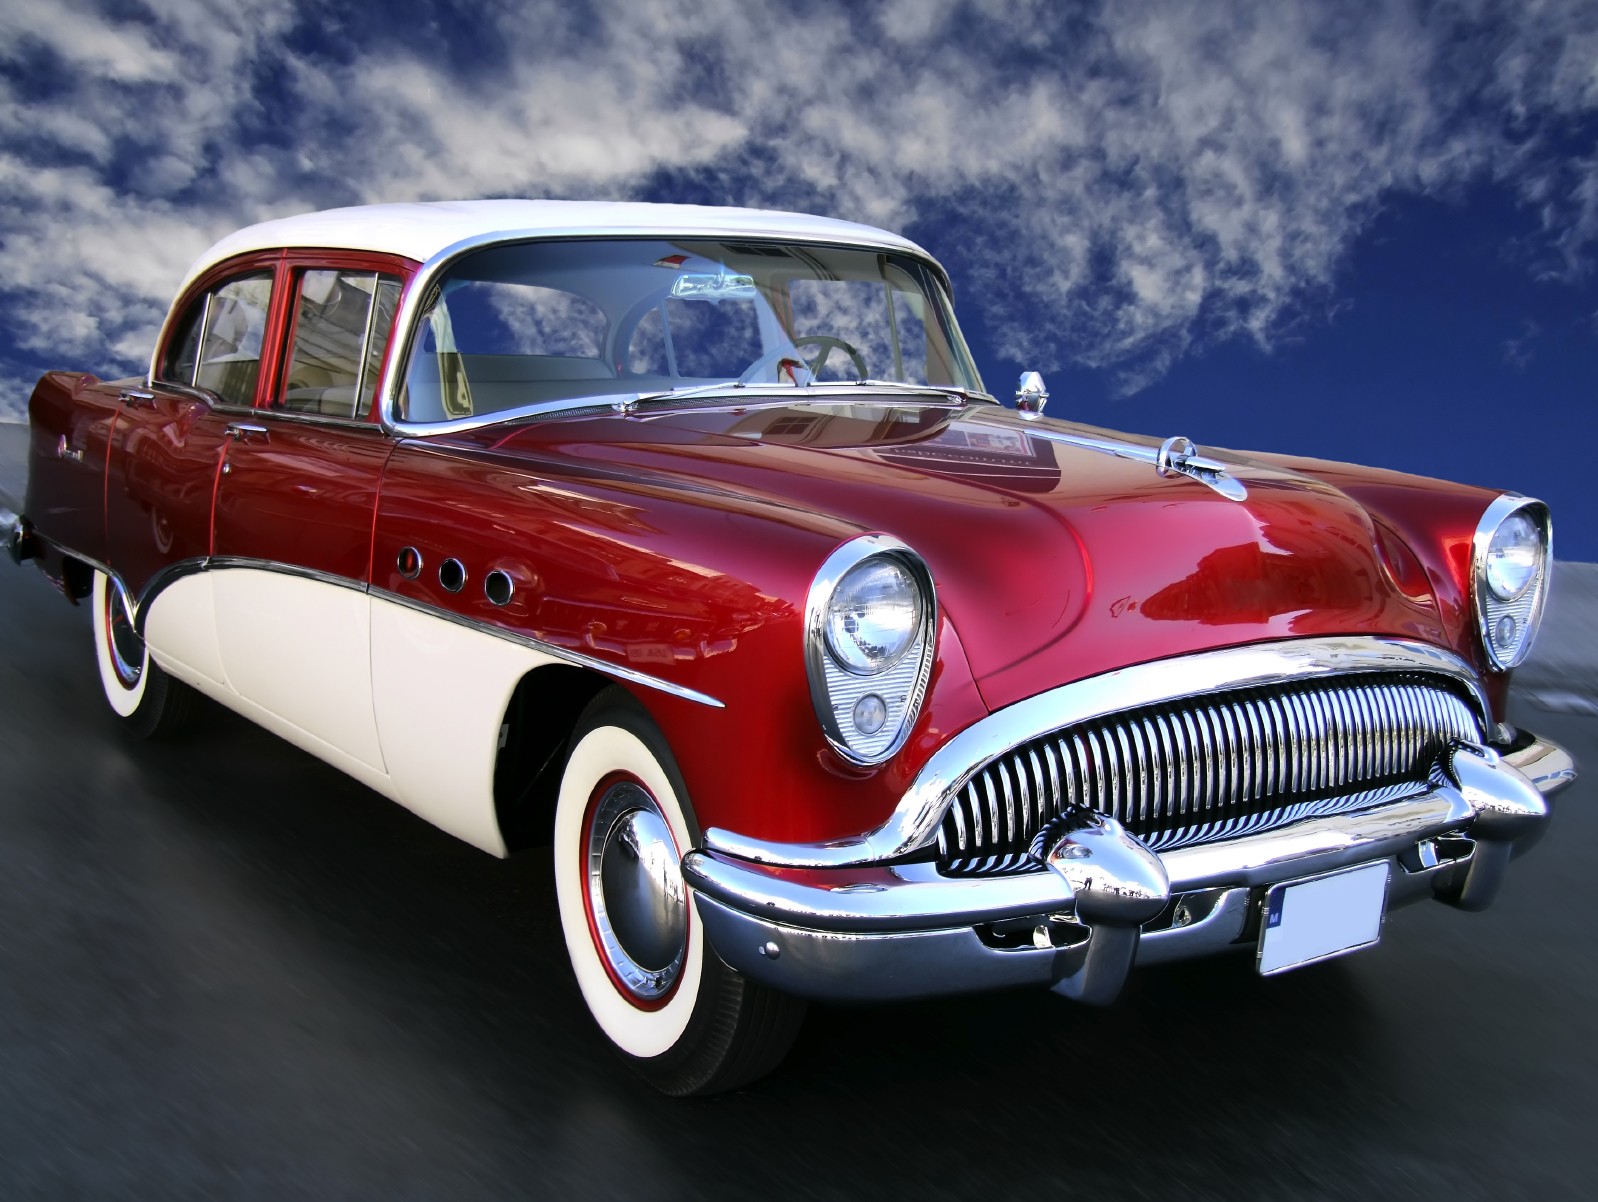
\includegraphics[width=\linewidth]{car.jpg} % content img num.1
	\end{subfigure}
	\begin{subfigure}[b]{0.225\linewidth}
		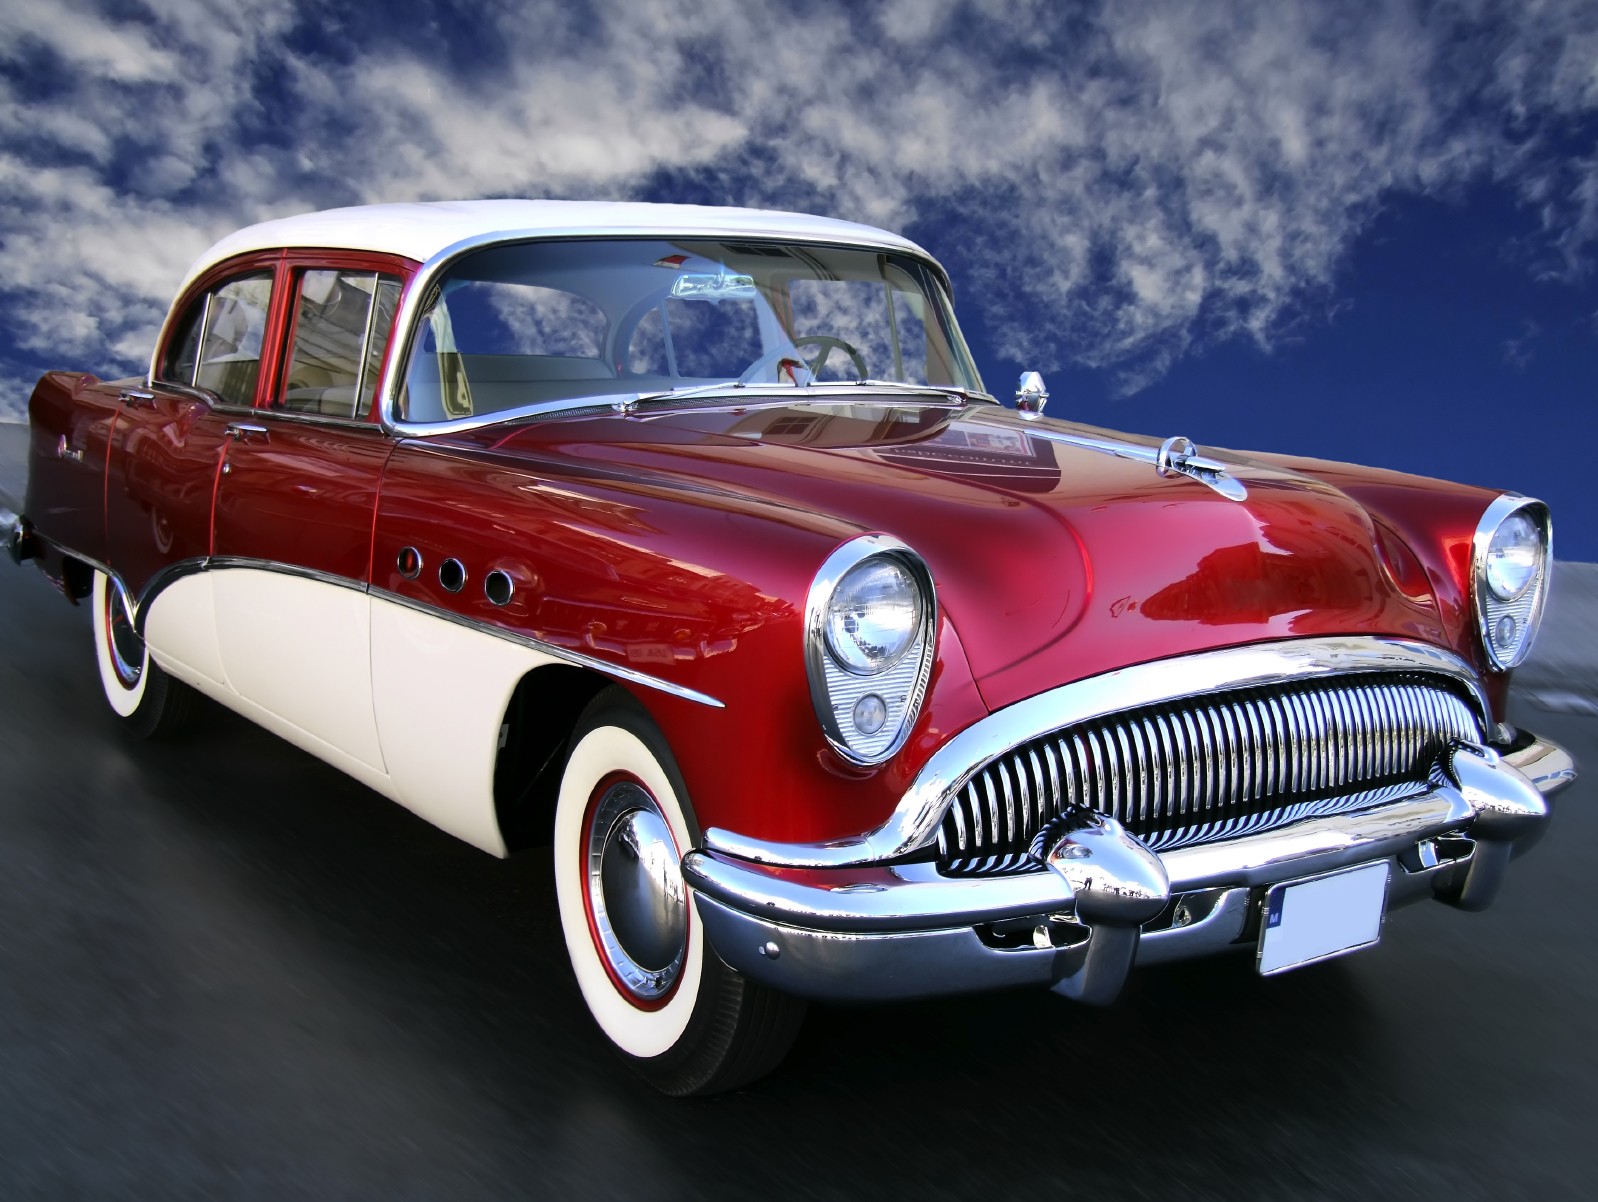
\includegraphics[width=\linewidth]{car.jpg} % regular UST num.1
	\end{subfigure}
	\begin{subfigure}[b]{0.225\linewidth}
		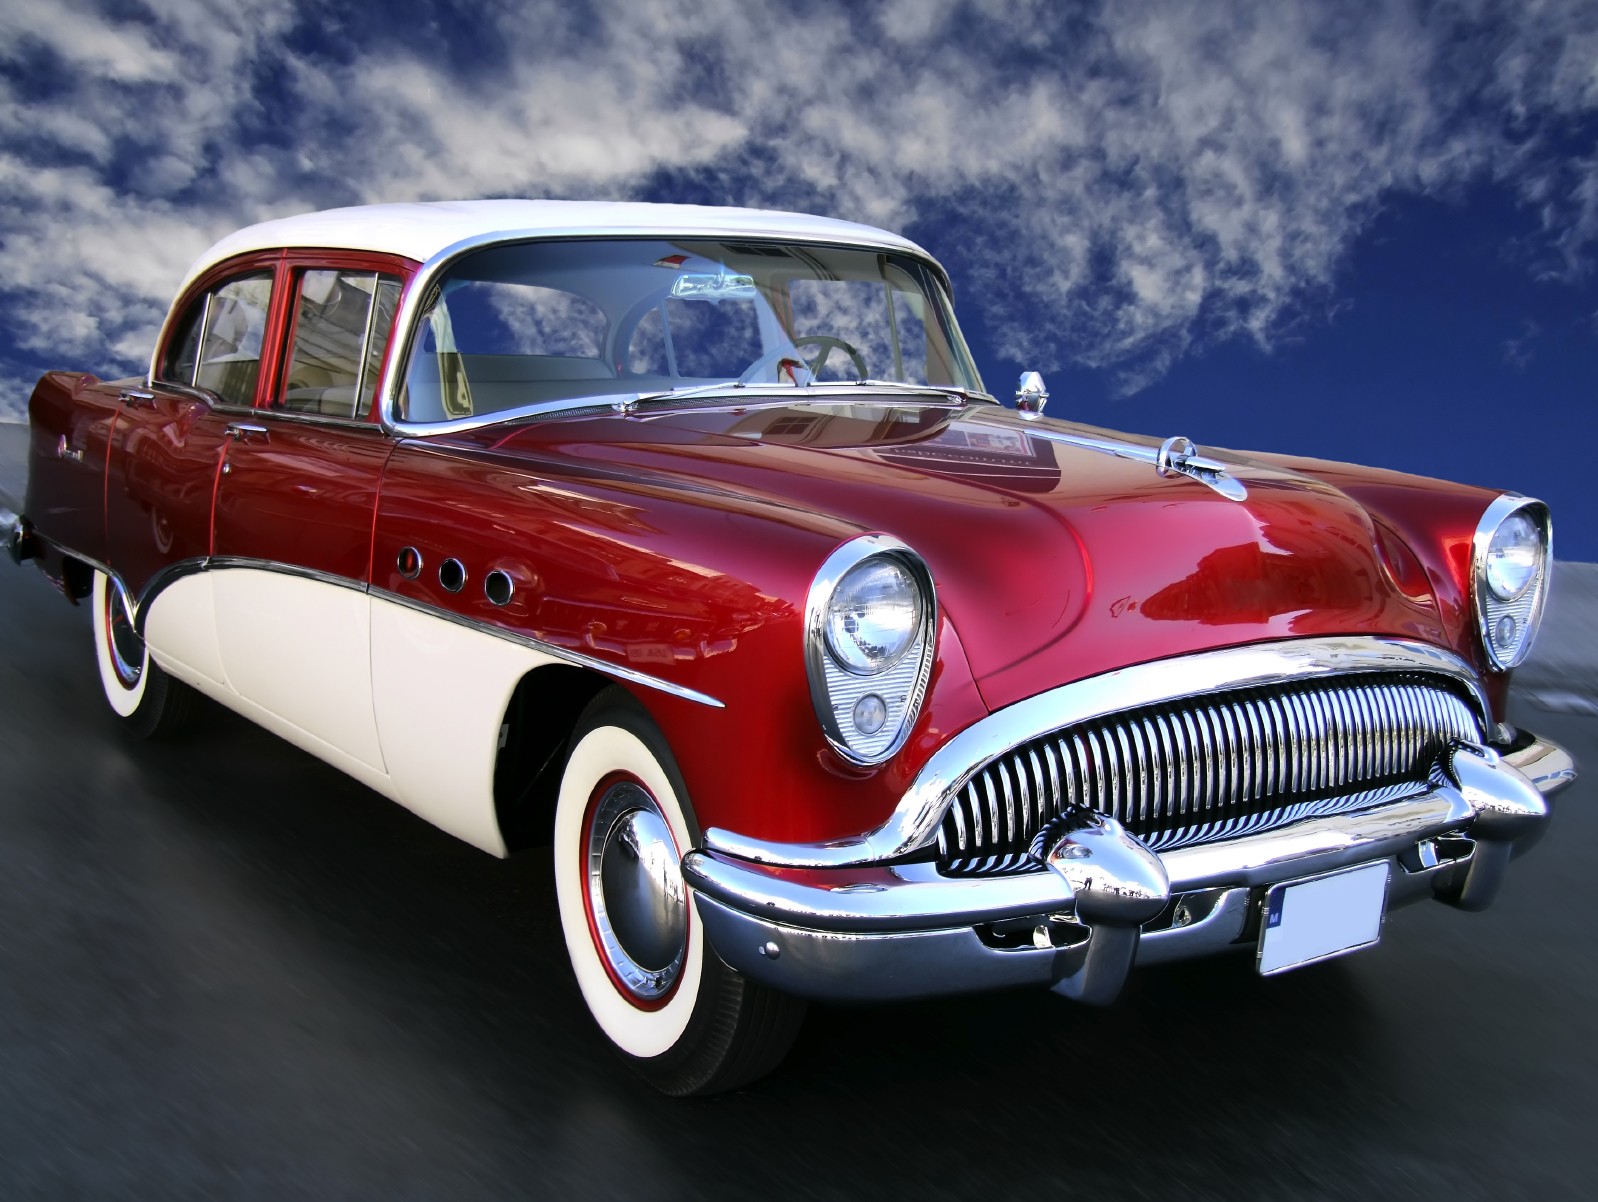
\includegraphics[width=\linewidth]{car.jpg} % UST+boost num.1
	\end{subfigure}
	% second line
	\centering
	\begin{subfigure}[b]{0.225\linewidth}
		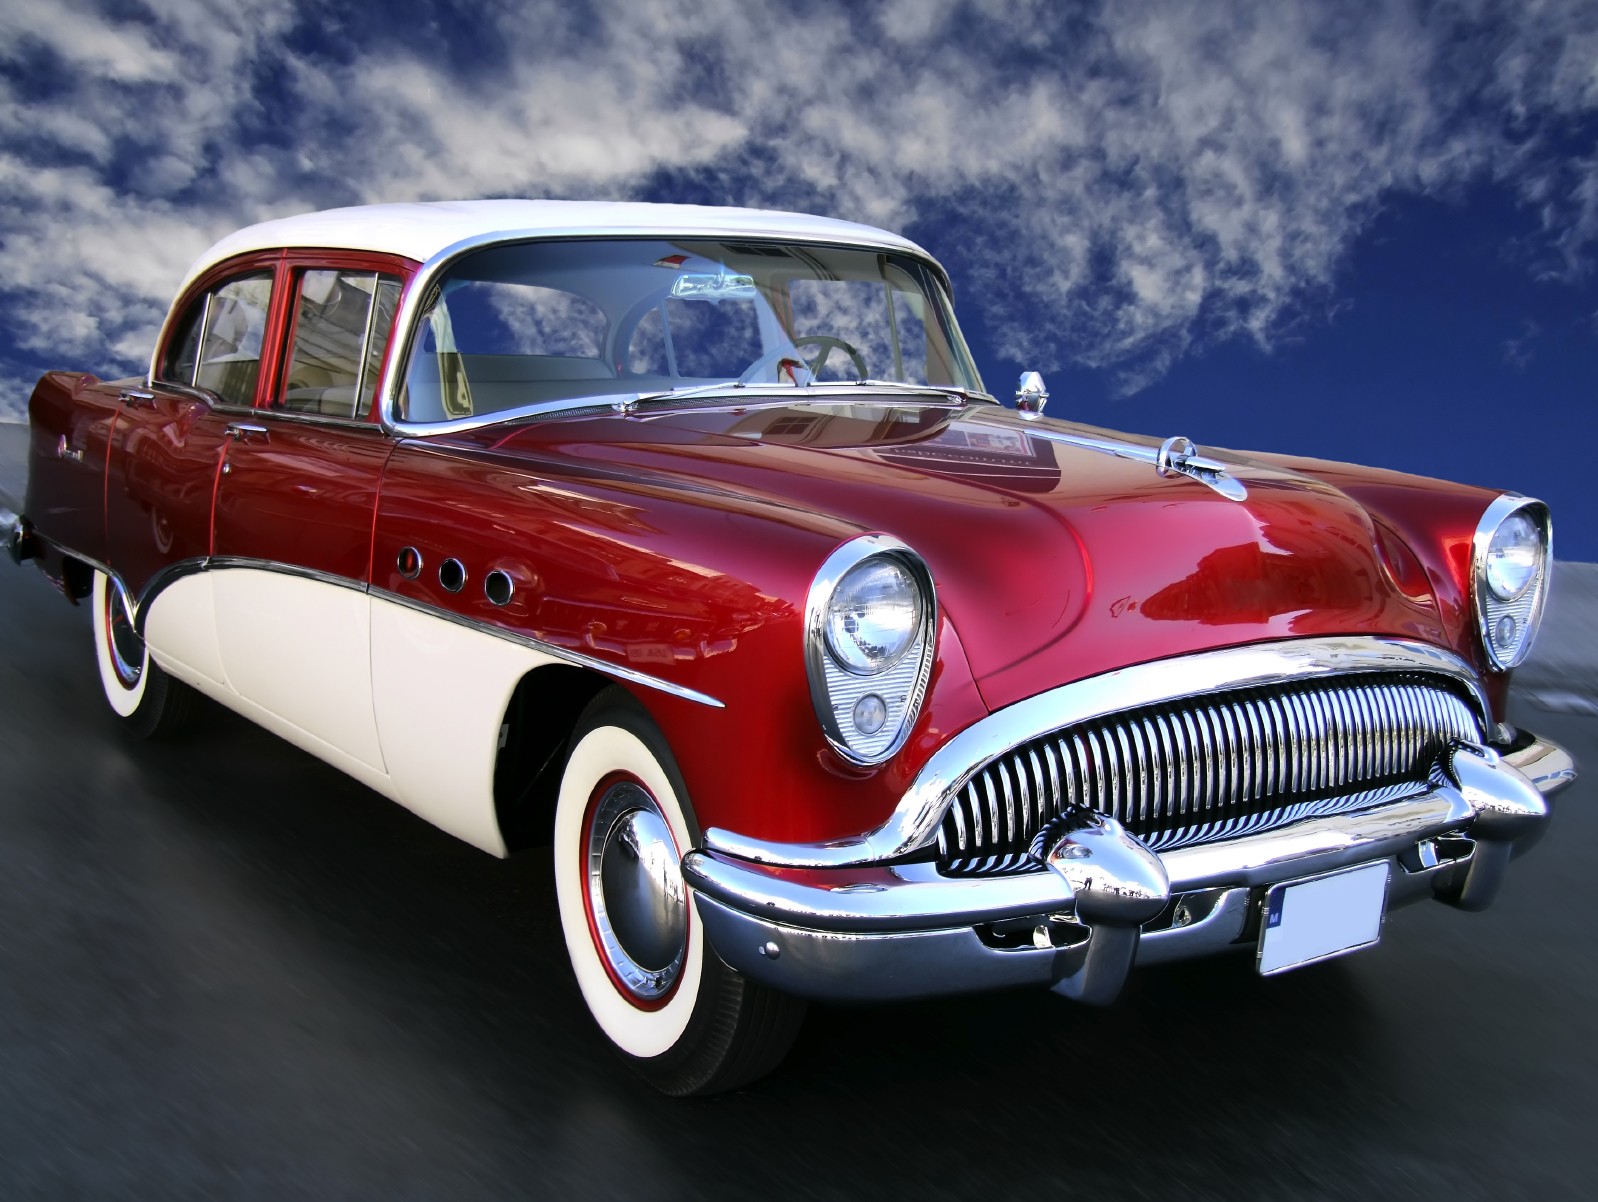
\includegraphics[width=\linewidth]{car.jpg} %style img num.2
	\end{subfigure}
	\begin{subfigure}[b]{0.225\linewidth}
		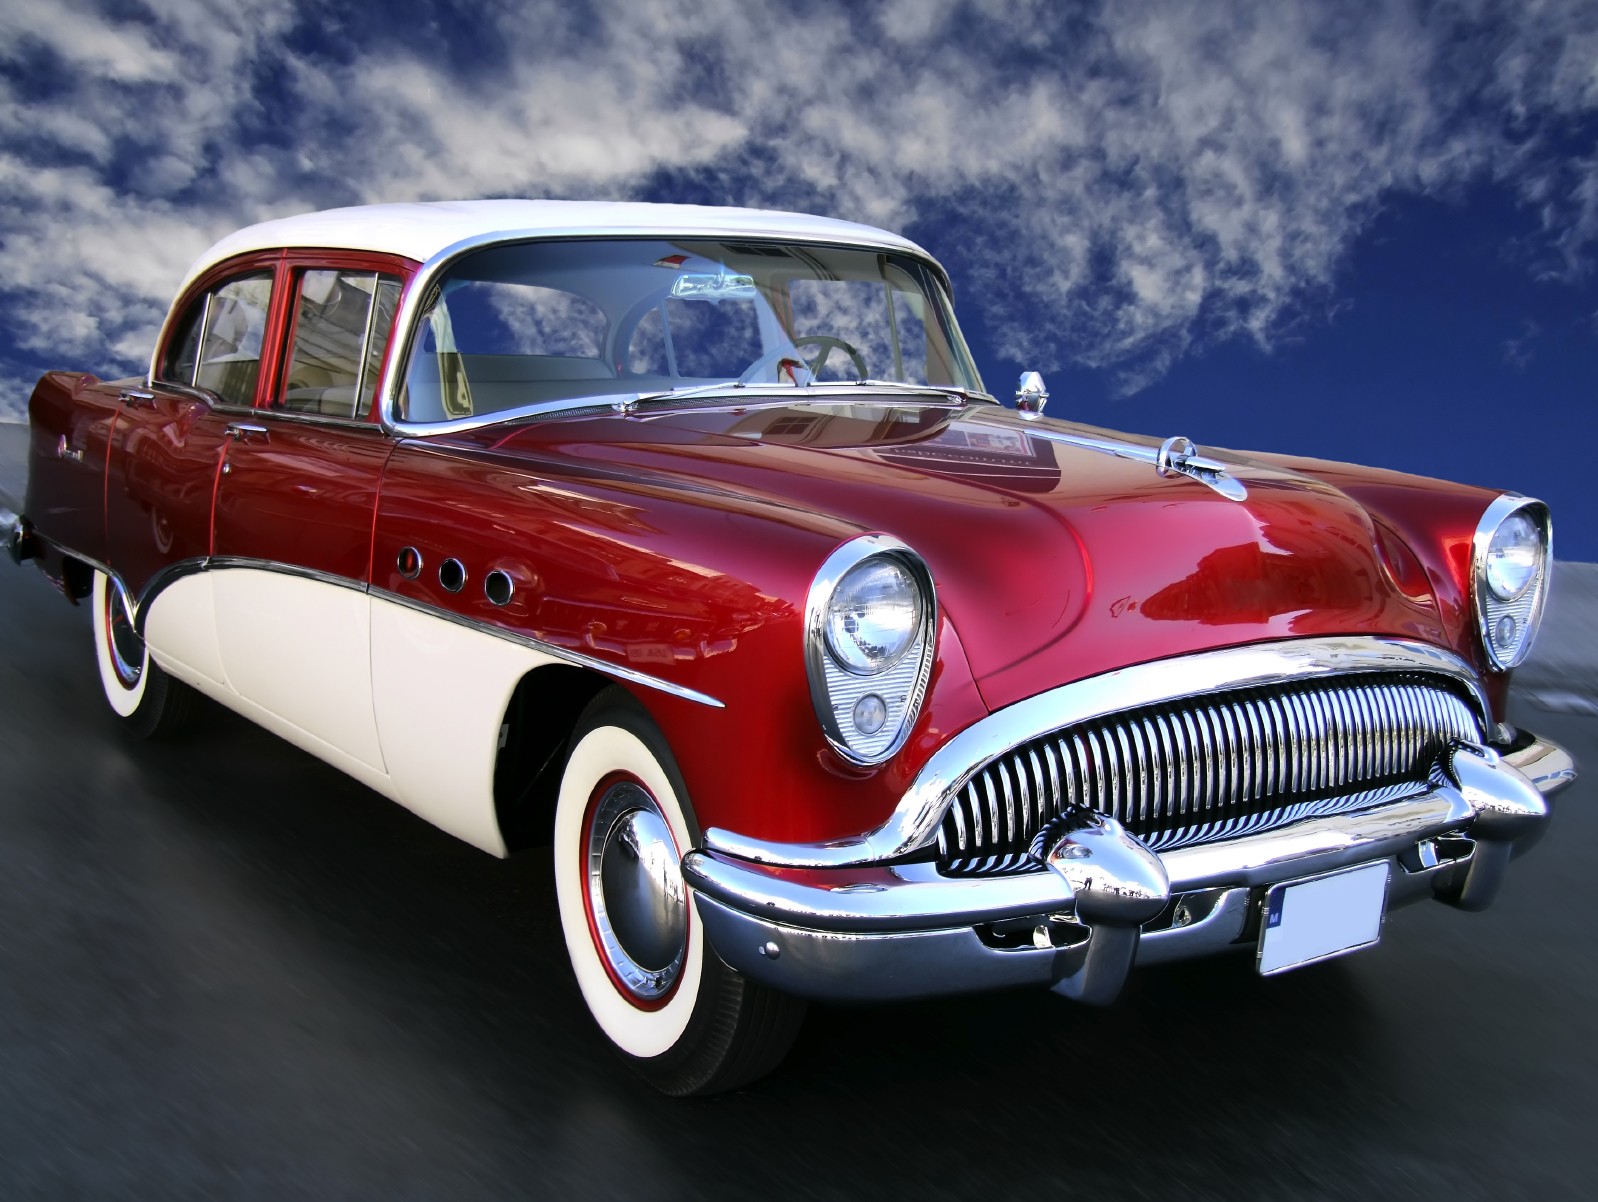
\includegraphics[width=\linewidth]{car.jpg} % content img num.2
	\end{subfigure}
	\begin{subfigure}[b]{0.225\linewidth}
		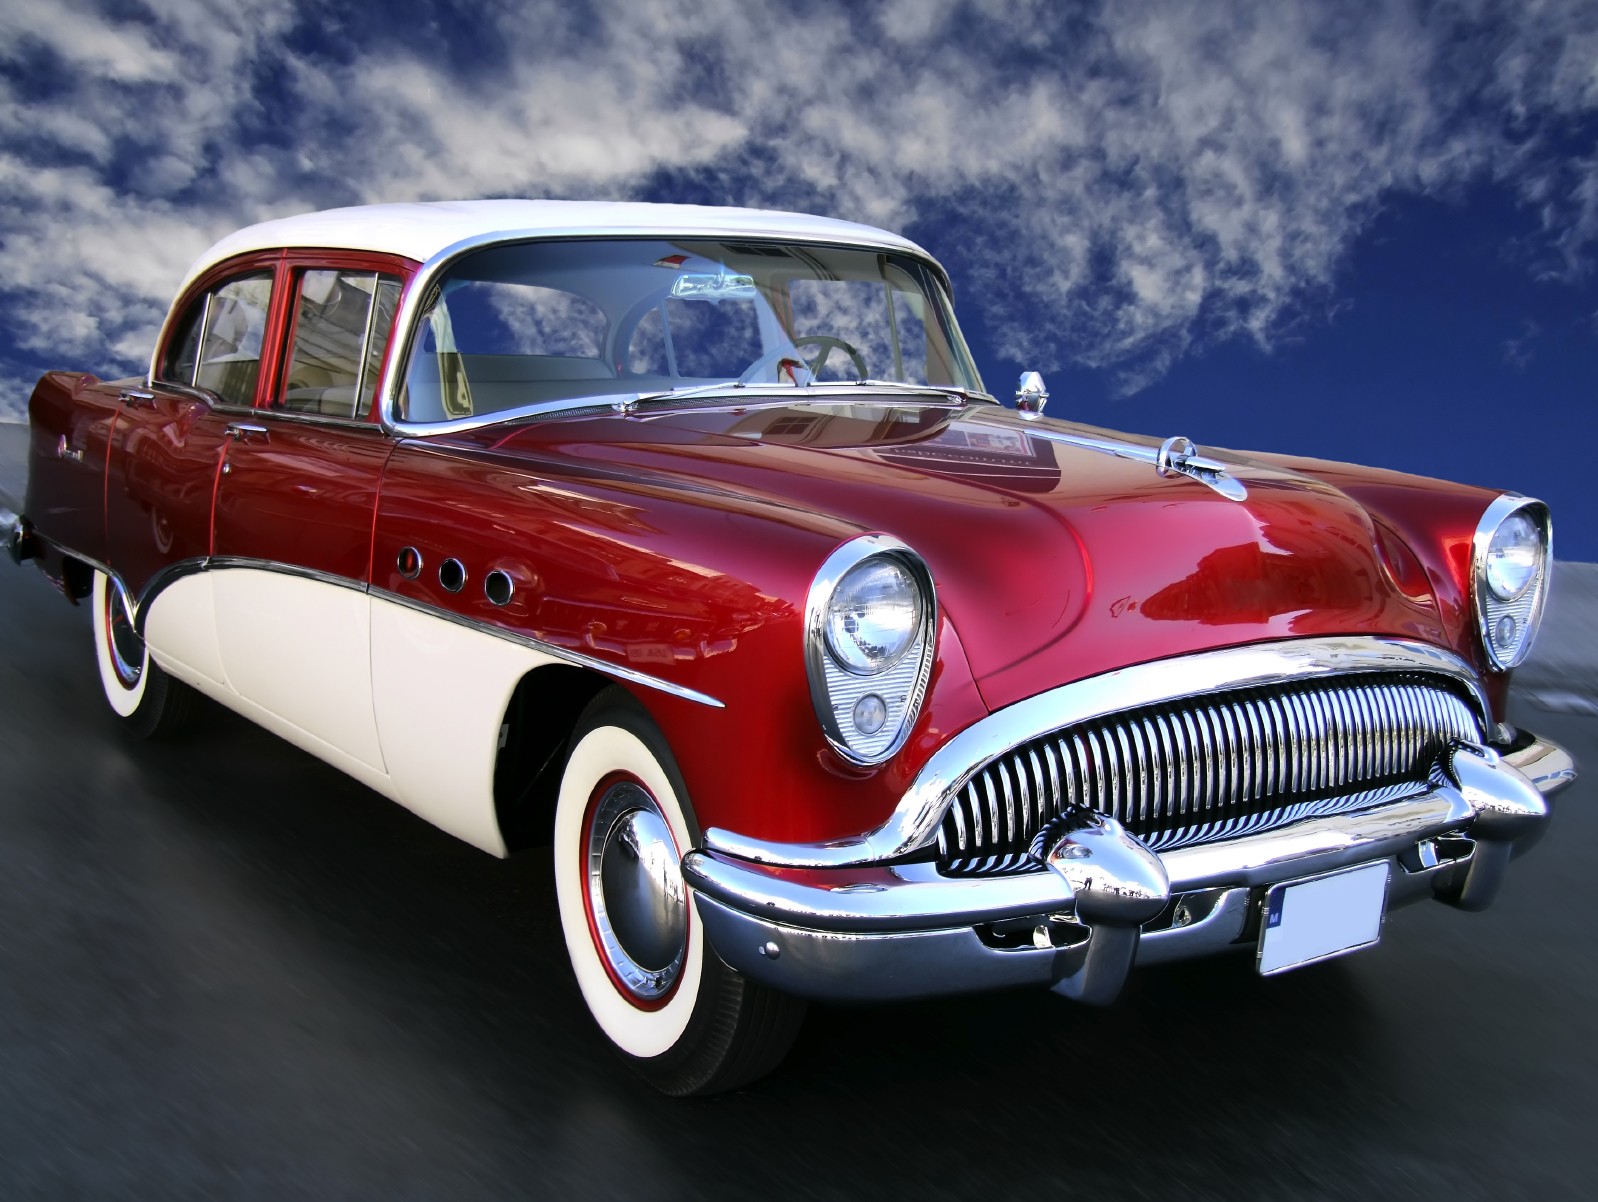
\includegraphics[width=\linewidth]{car.jpg} % regular UST num.2
	\end{subfigure}
	\begin{subfigure}[b]{0.225\linewidth}
		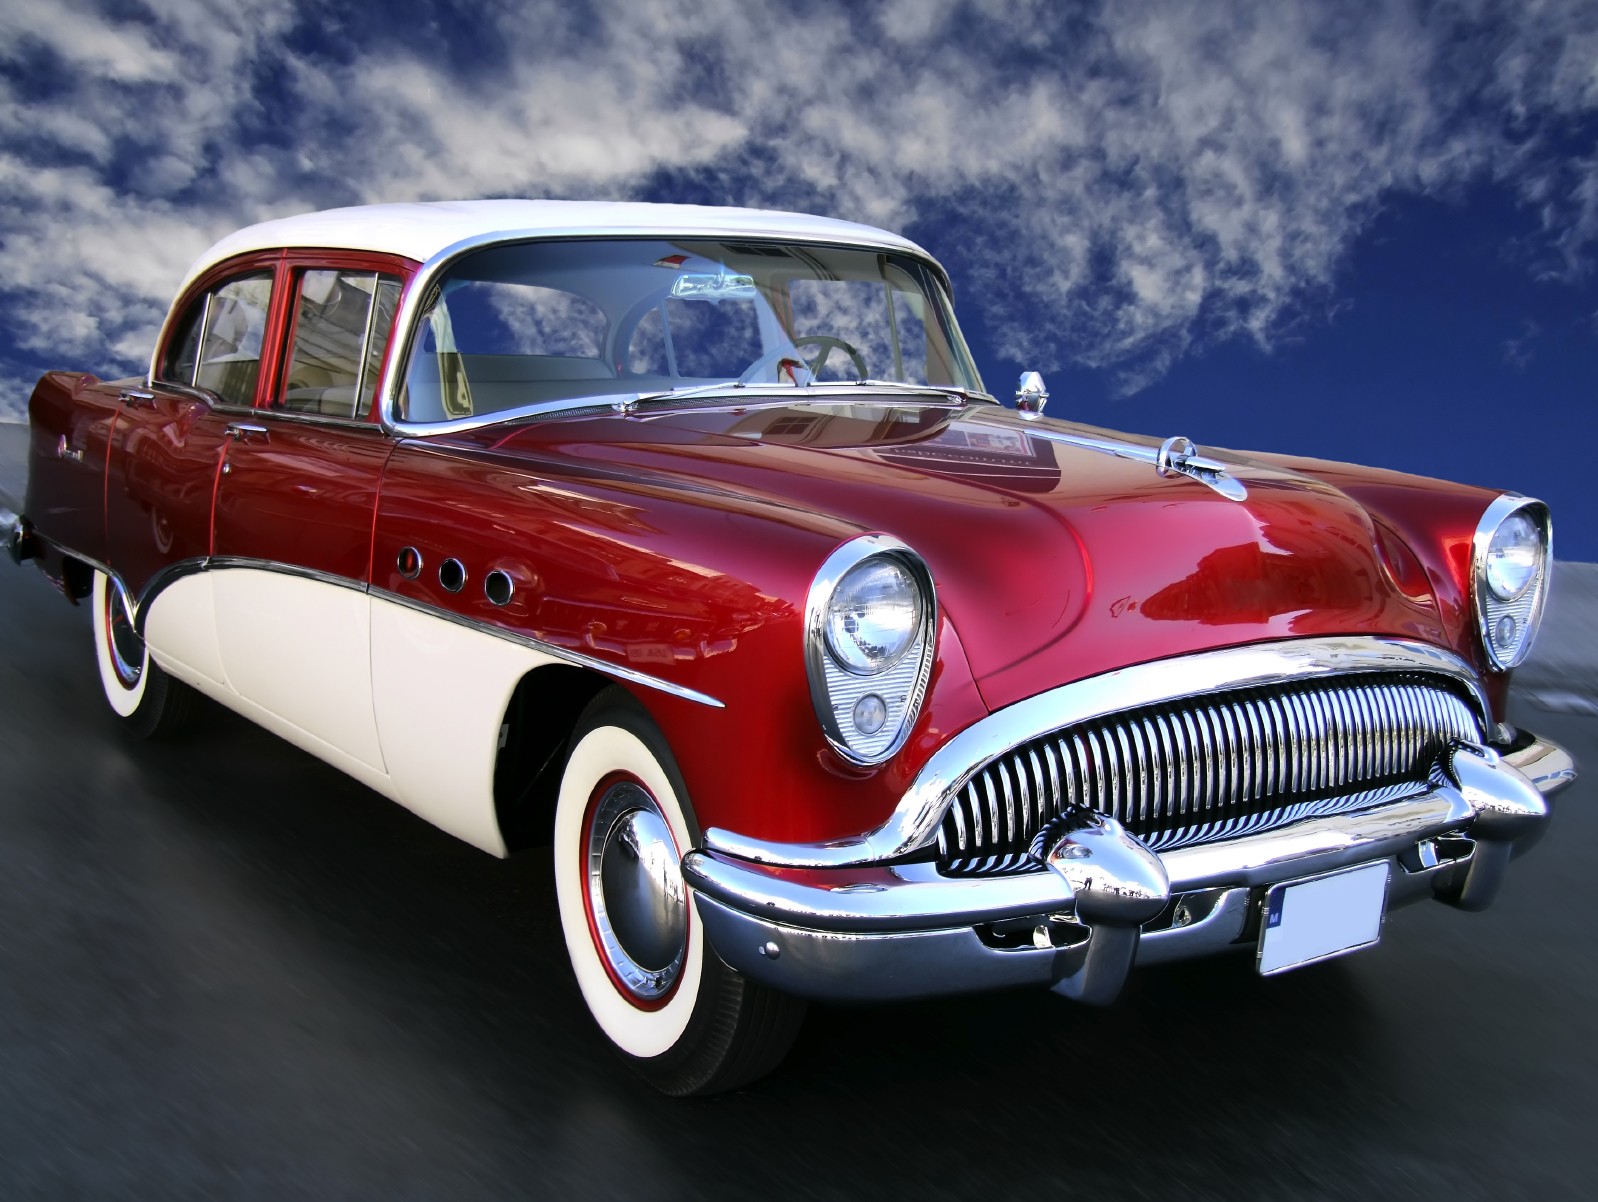
\includegraphics[width=\linewidth]{car.jpg} % UST+boos num.2
	\end{subfigure}
	% third line
	\centering
	\begin{subfigure}[b]{0.225\linewidth}
		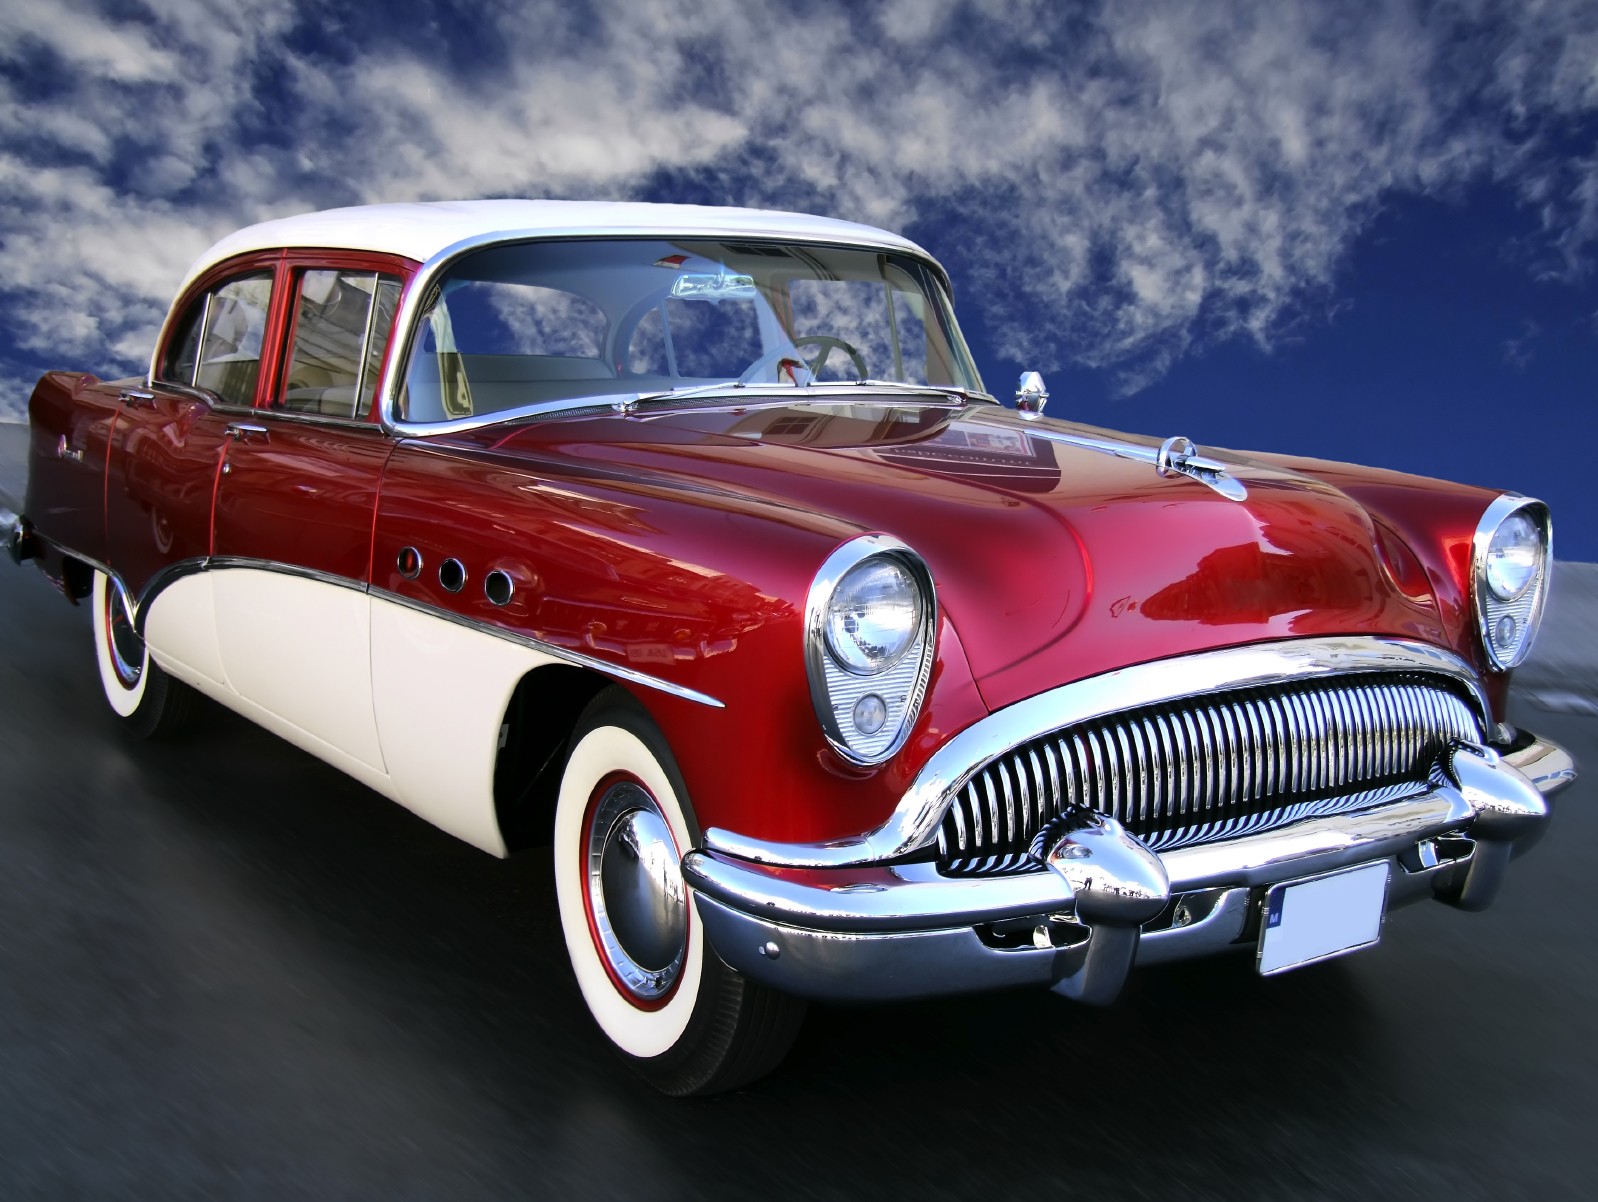
\includegraphics[width=\linewidth]{car.jpg} %style img num.3
		\caption{Style}
	\end{subfigure}
	\begin{subfigure}[b]{0.225\linewidth}
		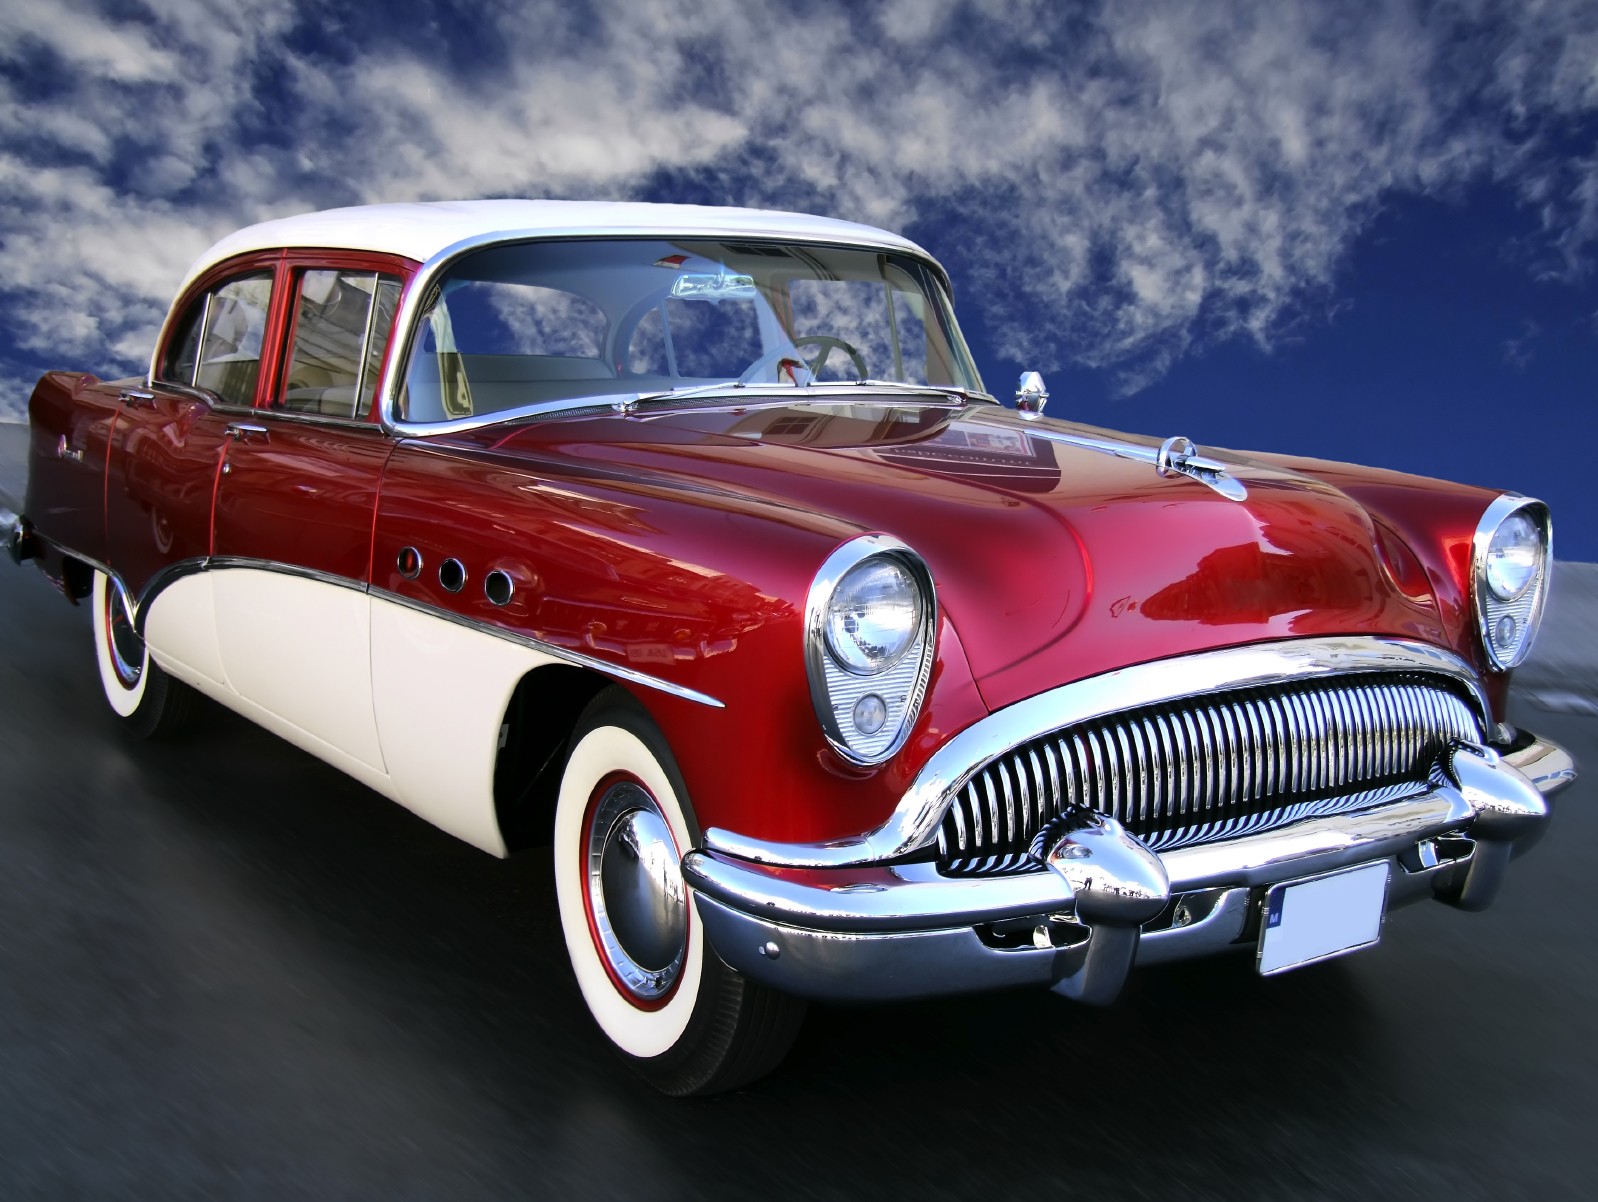
\includegraphics[width=\linewidth]{car.jpg} % content img num.3
		\caption{Content}
	\end{subfigure}
	\begin{subfigure}[b]{0.225\linewidth}
		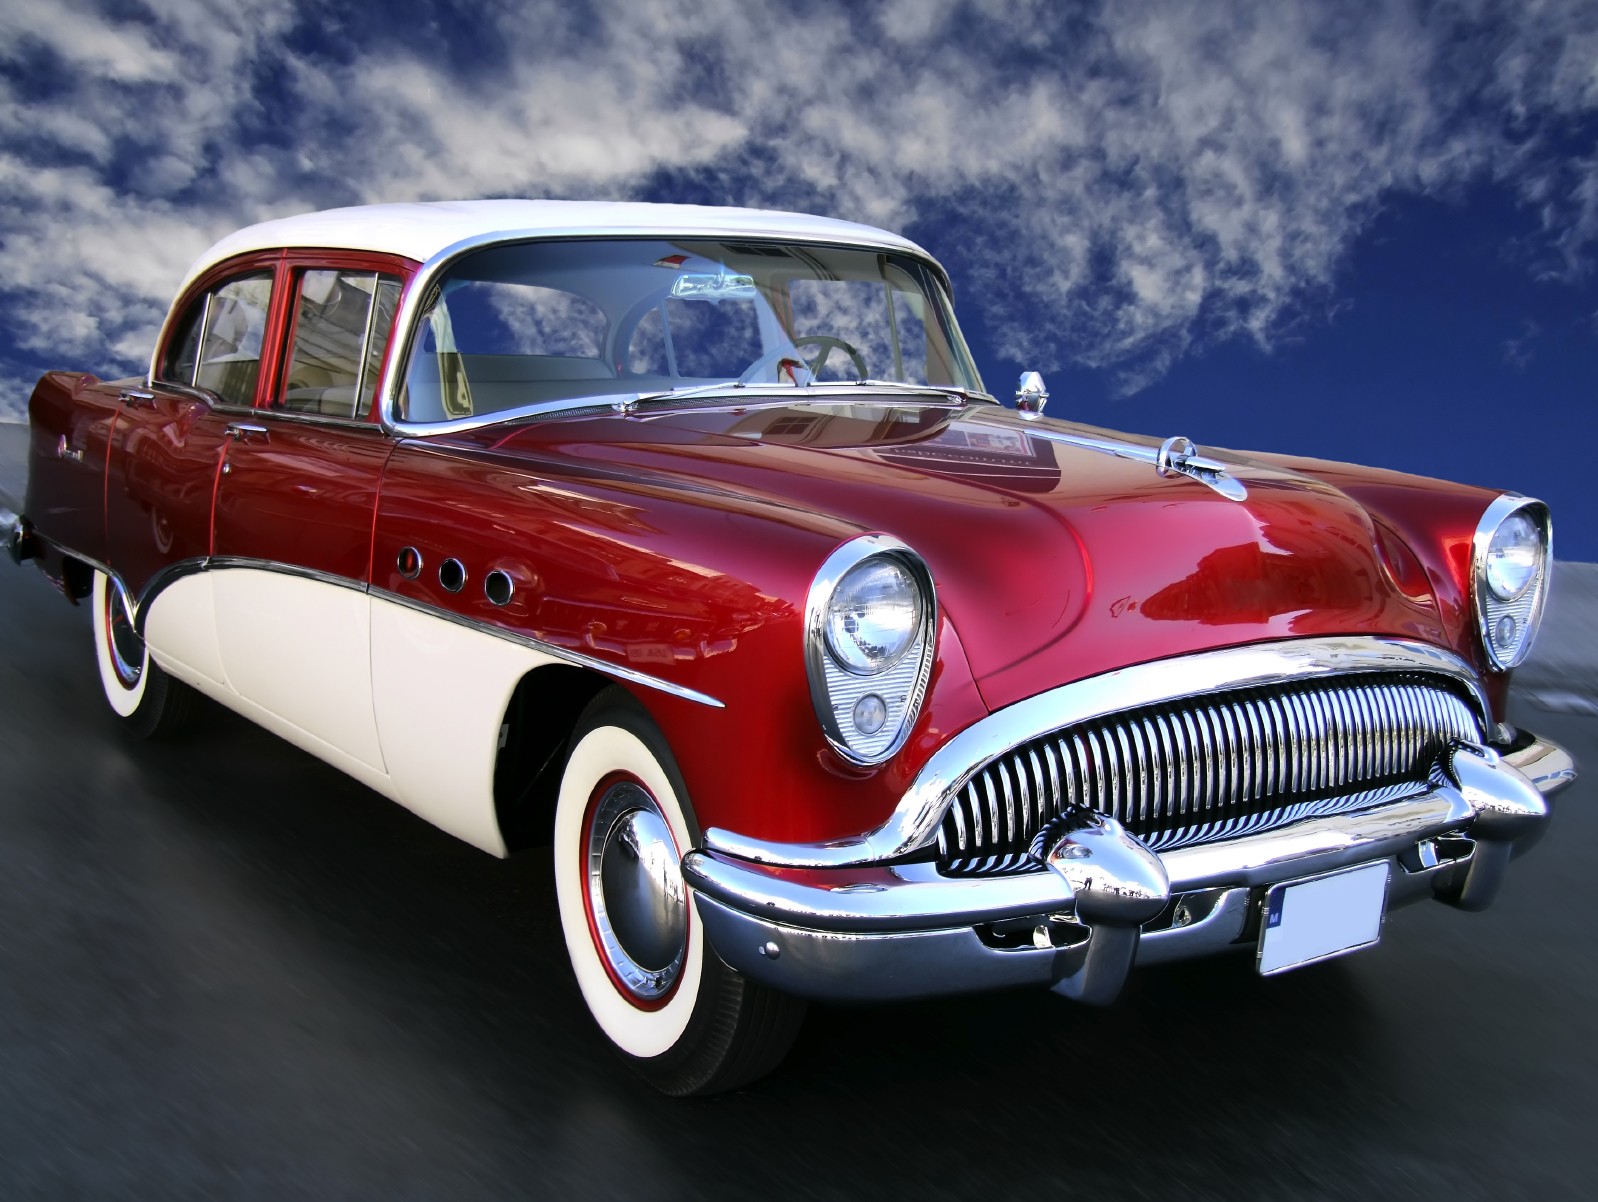
\includegraphics[width=\linewidth]{car.jpg} % regular UST num.3
		\caption{UST-Li et al. \cite{bib11}}
	\end{subfigure}
	\begin{subfigure}[b]{0.225\linewidth}
		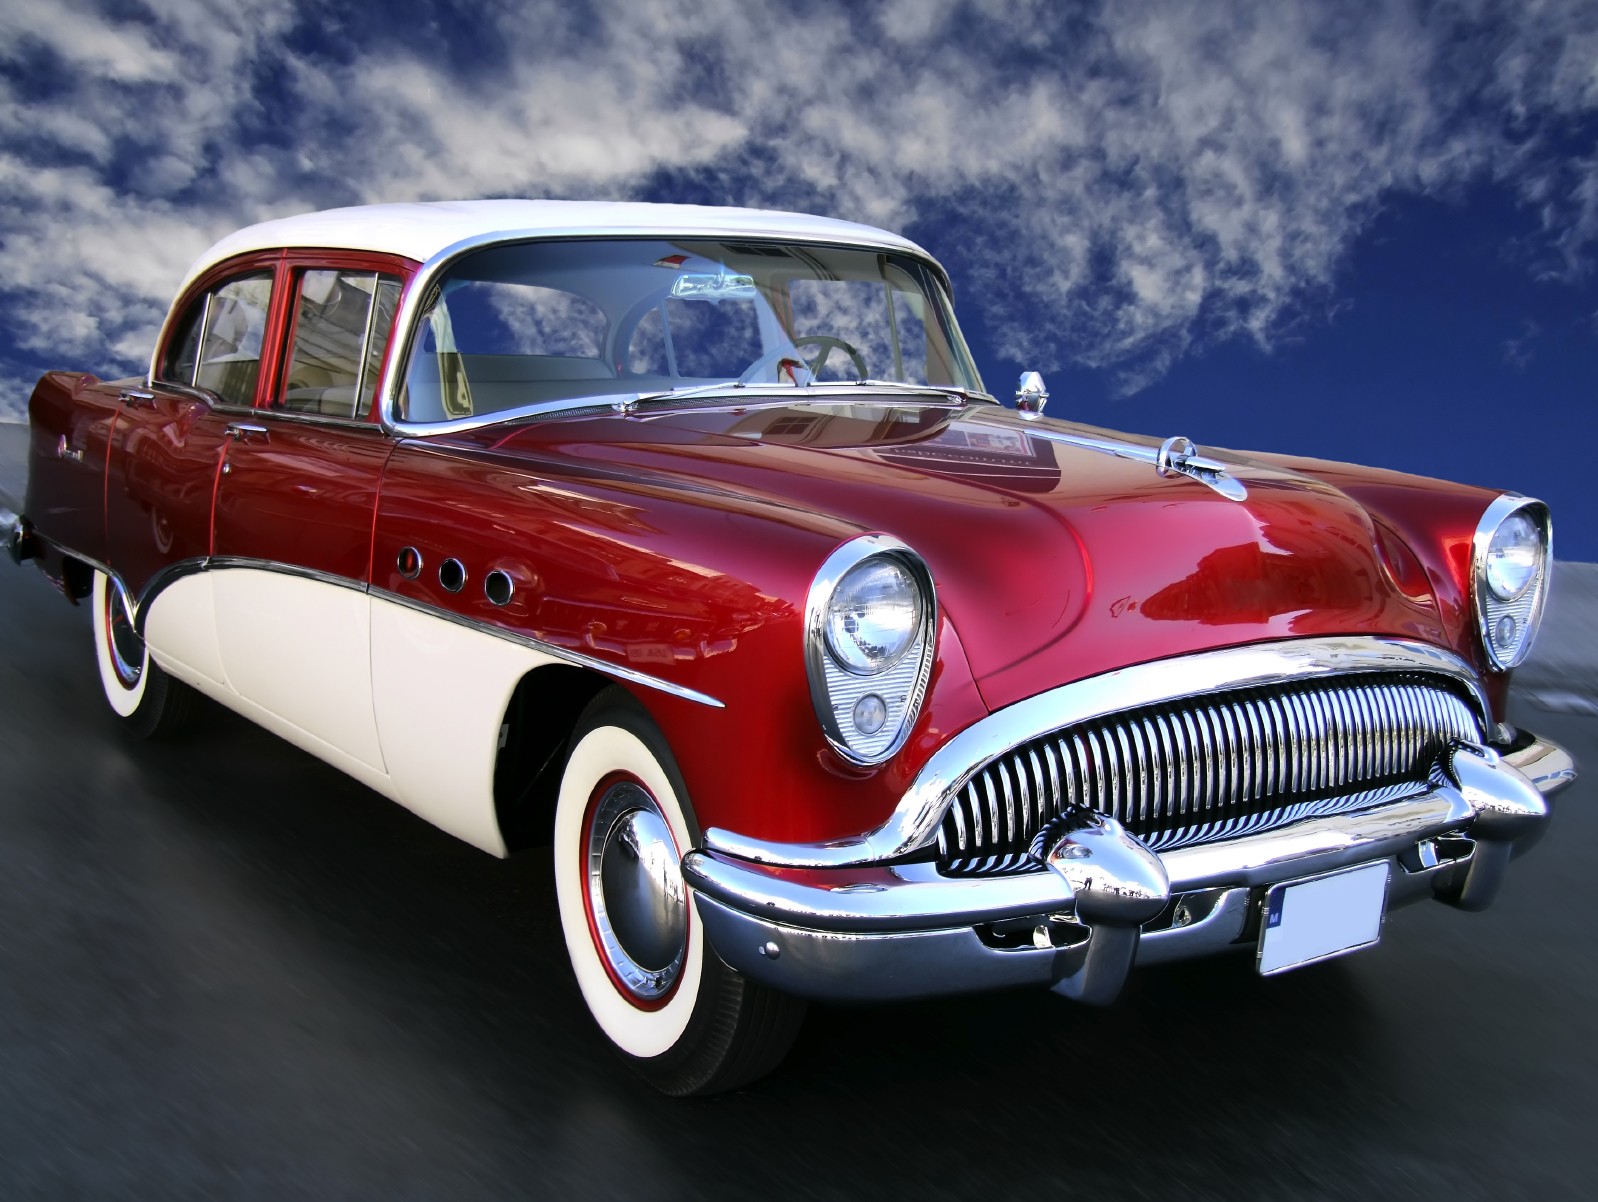
\includegraphics[width=\linewidth]{car.jpg} % UST+boos num.3
		\caption{UST+Boost}
	\end{subfigure}
	\caption{Results using Li et al. \cite{bib11} Encoder-Decoder architecture of UST, comparing our proposed method to boost stylization with the one Li et al. presented in \cite{bib11}.}
	\label{fig:Boost}
\end{figure}
% Merge  %
\begin{flushleft}
	\textbf{4.5 Two styles merging methods}\newline
\end{flushleft}
\begin{figure}[h!]
	% first line
	\centering
	\begin{subfigure}[b]{0.16\linewidth}
		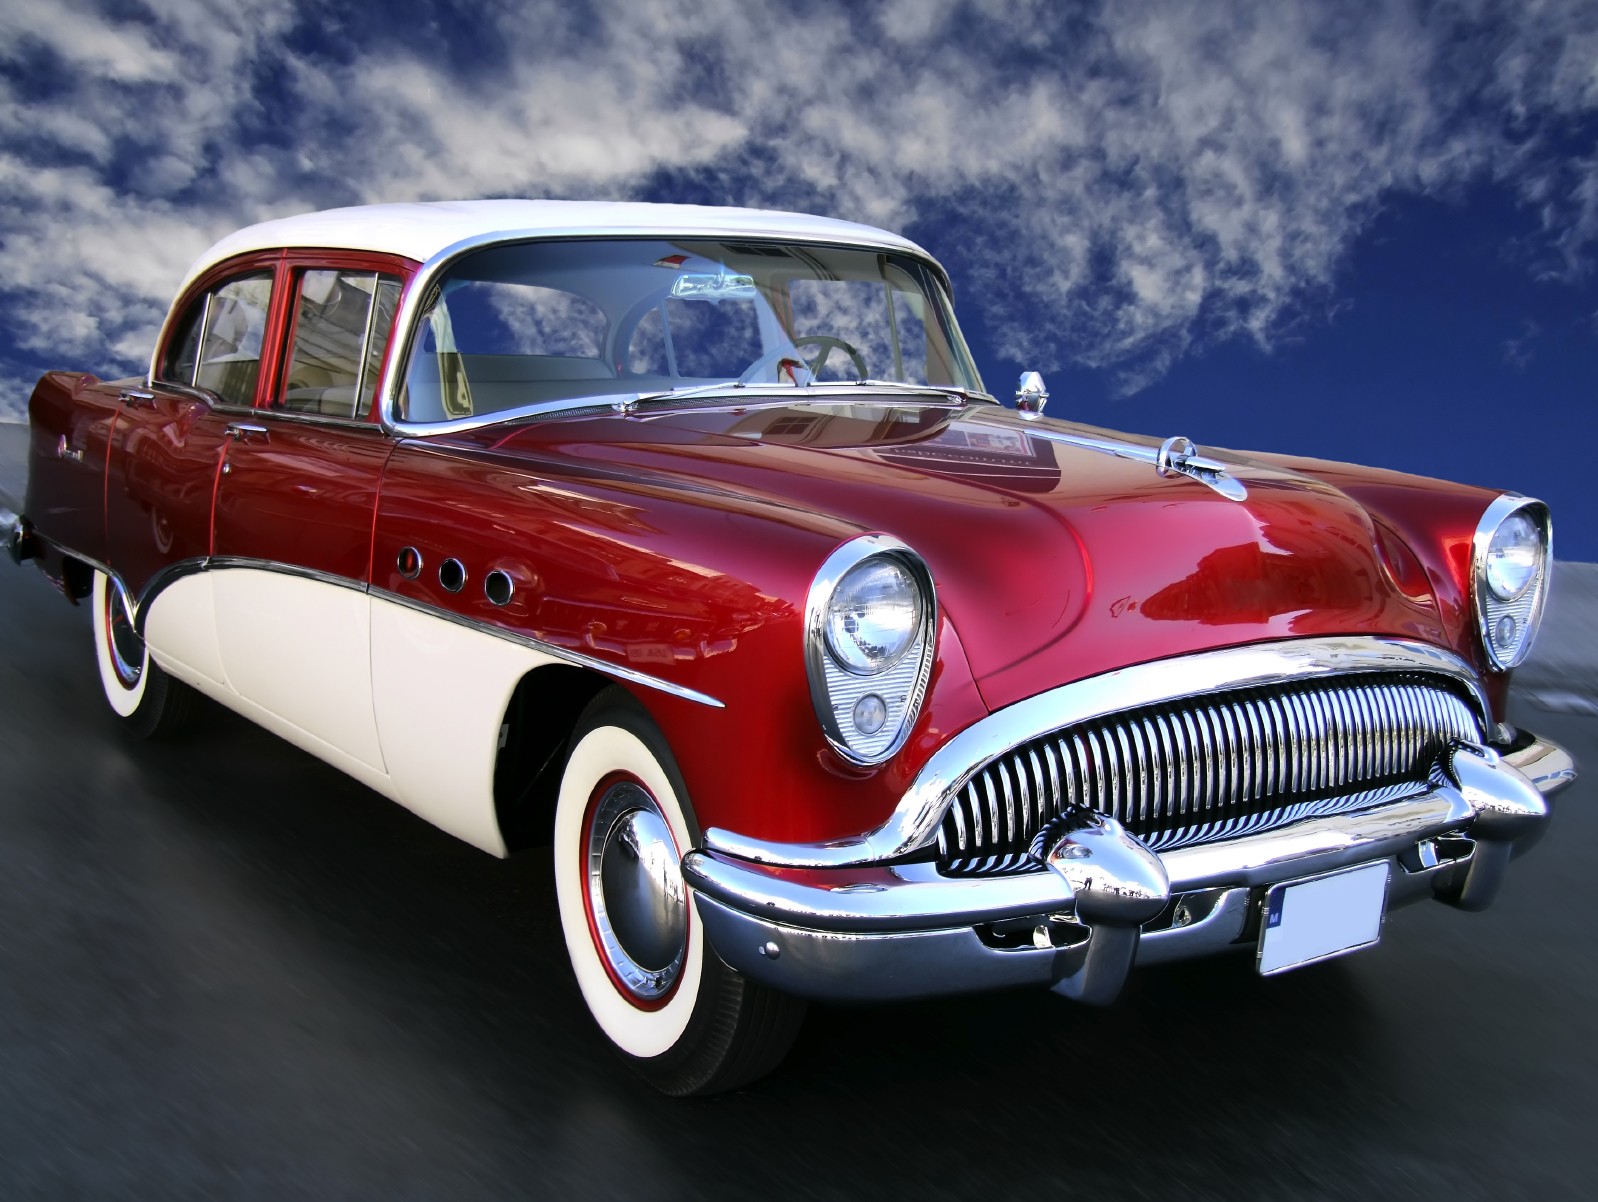
\includegraphics[width=\linewidth]{car.jpg} %style img num.1
	\end{subfigure}
	\begin{subfigure}[b]{0.16\linewidth}
		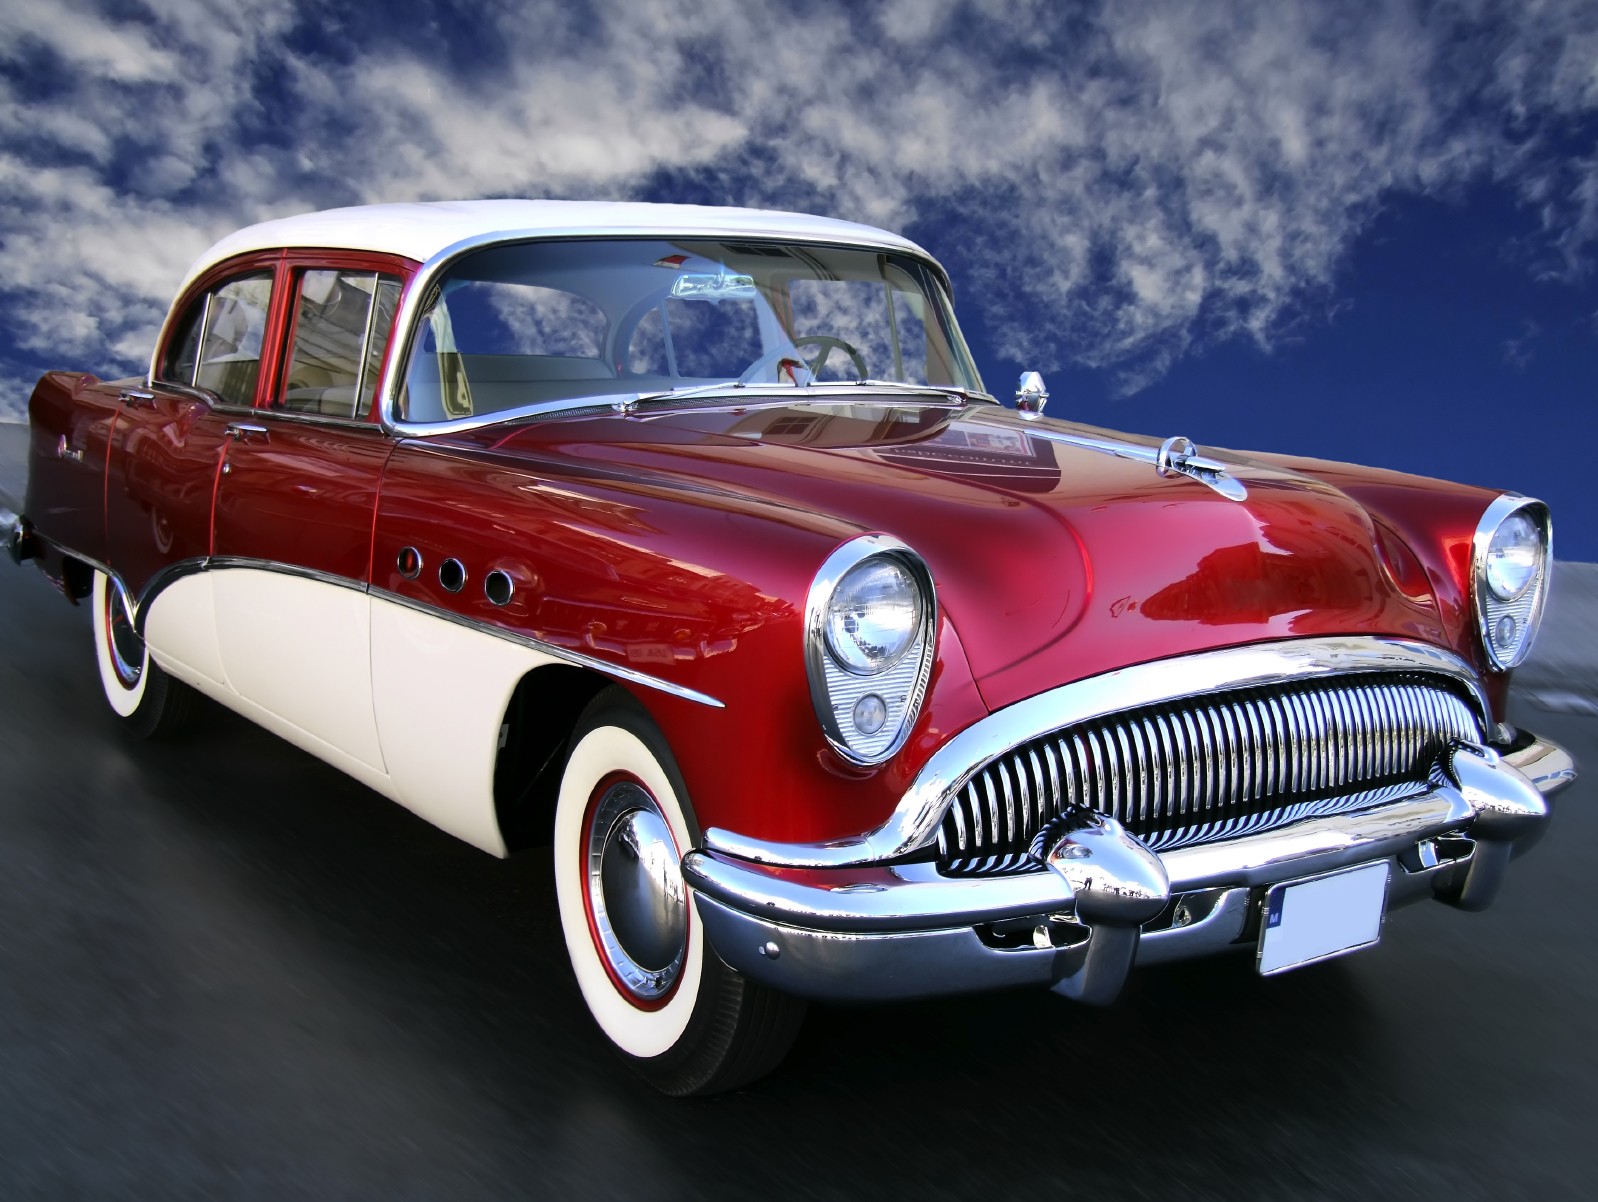
\includegraphics[width=\linewidth]{car.jpg} % content img num.1
	\end{subfigure}
	\begin{subfigure}[b]{0.16\linewidth}
		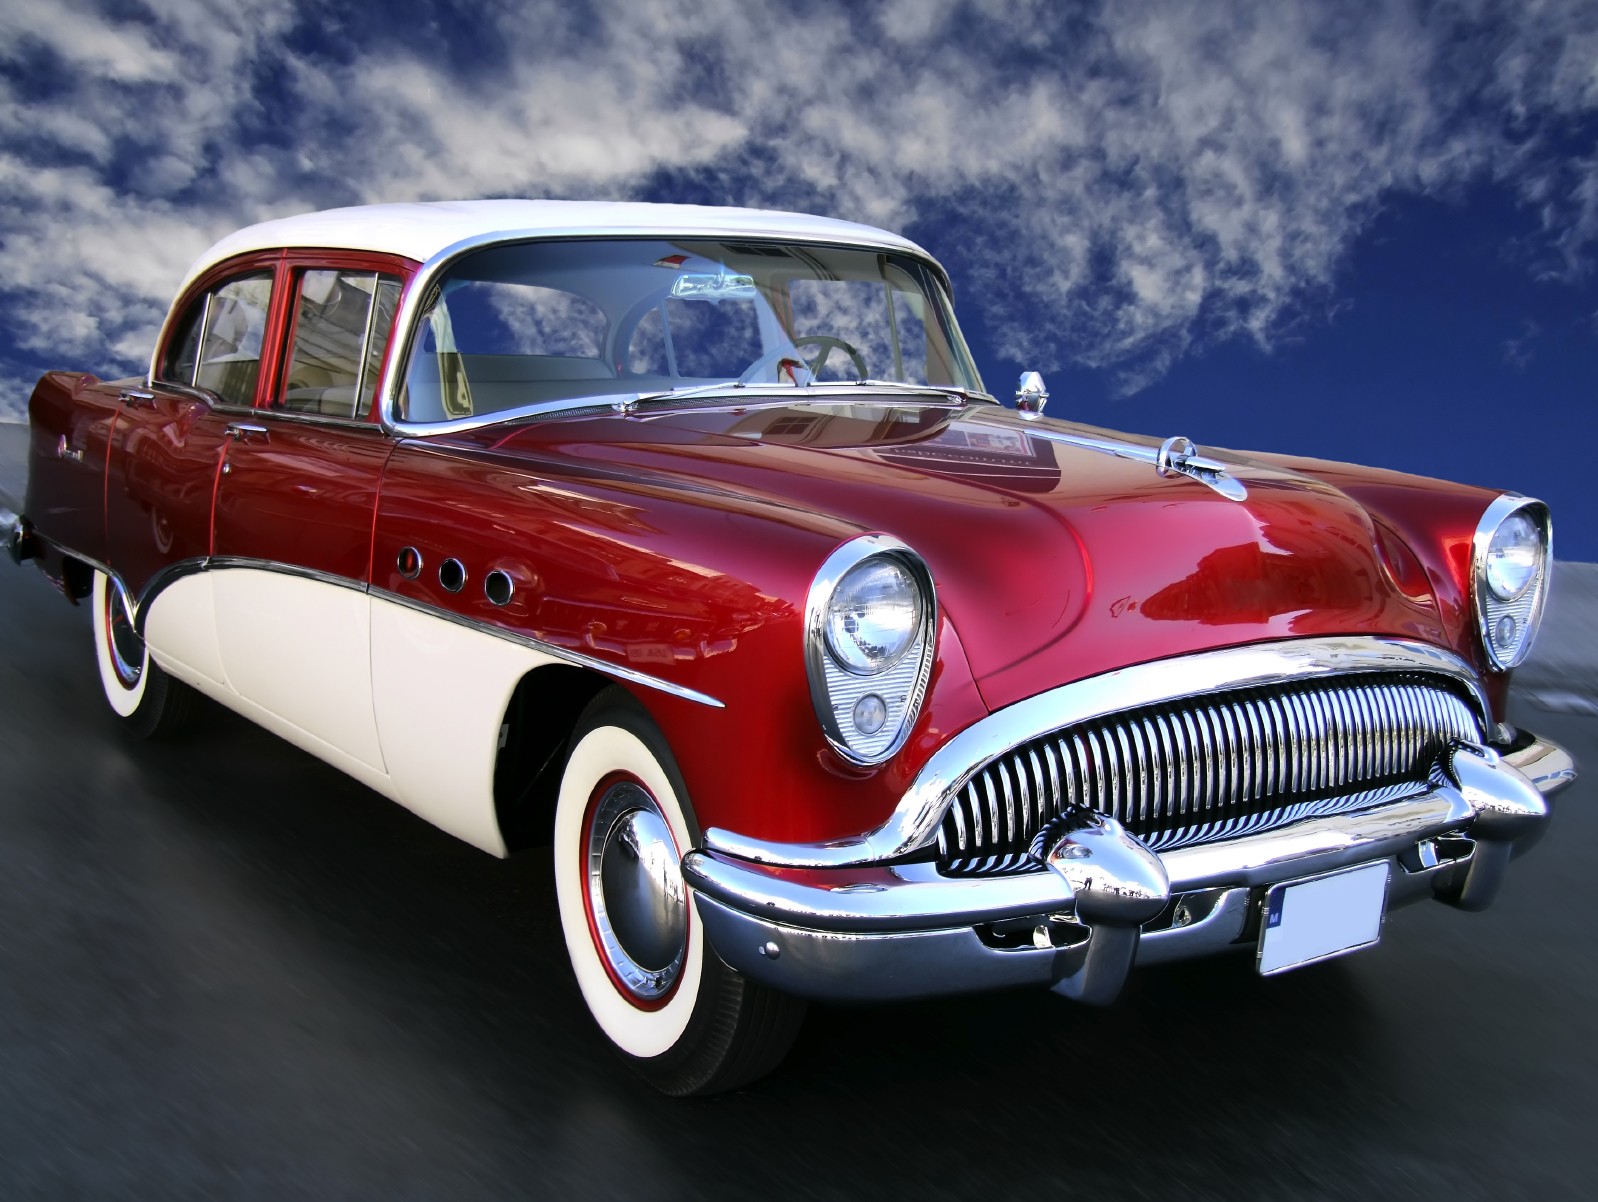
\includegraphics[width=\linewidth]{car.jpg} % orig merge num.1
	\end{subfigure}
	\begin{subfigure}[b]{0.16\linewidth}
		\includegraphics[width=\linewidth]{car.jpg} % merge1 num.1
	\end{subfigure}
	\begin{subfigure}[b]{0.16\linewidth}
		\includegraphics[width=\linewidth]{car.jpg} % merge2 num.1
	\end{subfigure}
	\begin{subfigure}[b]{0.16\linewidth}
		\includegraphics[width=\linewidth]{car.jpg} % merge3 num.1
	\end{subfigure}
	% second line
	\centering
	\begin{subfigure}[b]{0.16\linewidth}
		\includegraphics[width=\linewidth]{car.jpg} %style img num.2
	\end{subfigure}
	\begin{subfigure}[b]{0.16\linewidth}
		\includegraphics[width=\linewidth]{car.jpg} % content img num.2
	\end{subfigure}
	\begin{subfigure}[b]{0.16\linewidth}
		\includegraphics[width=\linewidth]{car.jpg} % orig merge num.2
	\end{subfigure}
	\begin{subfigure}[b]{0.16\linewidth}
		\includegraphics[width=\linewidth]{car.jpg} % merge1 num.2
	\end{subfigure}
	\begin{subfigure}[b]{0.16\linewidth}
		\includegraphics[width=\linewidth]{car.jpg} % merge2 num.2
	\end{subfigure}
	\begin{subfigure}[b]{0.16\linewidth}
		\includegraphics[width=\linewidth]{car.jpg} % merge3 num.2
	\end{subfigure}
	% third line
	\centering
	\begin{subfigure}[b]{0.16\linewidth}
		\includegraphics[width=\linewidth]{car.jpg} %style img num.3
		\caption{Style}
	\end{subfigure}
	\begin{subfigure}[b]{0.16\linewidth}
		\includegraphics[width=\linewidth]{car.jpg} % content img num.3
		\caption{Content}
	\end{subfigure}
	\begin{subfigure}[b]{0.16\linewidth}
		\includegraphics[width=\linewidth]{car.jpg} % orig merge num.3
		\caption{Li et al. \cite{bib11}}
	\end{subfigure}
	\begin{subfigure}[b]{0.16\linewidth}
		\includegraphics[width=\linewidth]{car.jpg} % merge1 num.3
		\caption{$1_{st}$ method}
	\end{subfigure}
	\begin{subfigure}[b]{0.16\linewidth}
		\includegraphics[width=\linewidth]{car.jpg} % merge2 num.3
		\caption{$2_{nd}$ method}
	\end{subfigure}
	\begin{subfigure}[b]{0.16\linewidth}
		\includegraphics[width=\linewidth]{car.jpg} % merge3 num.3
		\caption{$3_{rd}$ method}
	\end{subfigure}
		\caption{Results using Li et al. \cite{bib11} Encoder-Decoder architecture of UST, comparing our proposed method to boost stylization with the one Li et al. presented in \cite{bib11}.}
		\label{fig:Merge}
\end{figure}
add more text here
add texture synthesis 